\documentclass[10pt, xcolor={dvipsnames}, aspectratio=169]{beamer}
\usepackage[utf8]{inputenc}
\usepackage[super, square]{natbib}
\usepackage{mathtools, relsize, graphicx, amssymb, amsthm}
\usepackage{listings}
\usepackage{color}
\usepackage[strings]{underscore}

\lstset{
    frame=single,
    basicstyle=\footnotesize,
    keywordstyle=\color{purple},
    numbers=left,
    numbersep=5pt,
    showstringspaces=false, 
    stringstyle=\color{blue},
    tabsize=4,
    language=C++
}

\mode<presentation>{\usetheme{Berlin} \usecolortheme{beetle}}

\title{Parallel Sorting of Roughly-Sorted Sequences}
\author{Anthony Pfaff, Jason Treadwell}
\institute{CSCI 5172 $|$ CU Denver $|$ Fall '16}
\date{12.10.2016}

\begin{document}
\setbeamertemplate{navigation symbols}{} %remove navigation symbols
\bibliographystyle{plain}
\nocite{*}
% gets rid of the references button
\renewcommand{\bibsection}{\subsubsection*{\bibname}}
\graphicspath{{./}}

\begin{frame}
\titlepage
\end{frame}

\begin{frame}
\transfade
\frametitle{Introduction}
Sorting a sequence according to some ordering is a foundational problem of computer science. \newline

Sorting has crucial and non-obvious applications. There exist a great many such algorithms. \newline

The optimal runtime of sorting a sequence of length $n$ by \textit{comparison} is $\Theta(n \lg n)$.
\end{frame}

\begin{frame}
\frametitle{Sort Algorithms}
The comparison sorts include Mergesort, Heapsort, Quicksort, etc.\ and have diverse strengths. \newline

The former two are asymptotically optimal; Quicksort frequently outruns them, but is $O(n^2)$. \newline

We can beat the linearithmic runtime bounds through additional analysis of the input array.
\end{frame}

\begin{frame}
\frametitle{Roughly-Sorted Sequences}
The sequence $A = \{a_0, a_1, \cdots, a_{n-1}\}$ is $k$-sorted if it satisfies
$$a_i \leq a_j \quad\forall\; i < j - k\,,\quad 0 \leq i \leq j < n \,.$$ \newline

The radius of $A$ is the smallest $k$ such that $A$ is $k$-sorted:
$$\text{radius}(A) = \max\{j - i \mid j > i,\, a_i > a_j \} \,.$$
\end{frame}

\begin{frame}
\frametitle{Conventions}
We'll only consider sequences of 32-bit integers backed by \textit{random-access arrays}. \newline

The array $A = \{a_0, a_1, \cdots, a_{n-1}\}$ is \textit{sorted} if its elements are all ordered in nondecreasing order. \newline

When we say $A$ is $k$-sorted, we imply that $k$ is minimal (i.e., the radius of $A$ is $k$).
\end{frame}

\begin{frame}
\frametitle{Roughly-Sorted Sequences (cont.)}
Some applications involve sorted arrays that become slightly perturbed. \newline

We might be able to exploit their partial sortedness to beat the $\Omega(n \lg n)$ lower runtime bound. \newline

Comparison-based sorts are prone to divide-and-conquer and rife with opportunities for parallel speedup.
\end{frame}

\begin{frame}
\frametitle{Roughsort}
Roughsort exploits the presortedness of the array $A$ by applying a radius \textit{halving} algorithm. \newline

The algorithm sorts $A$ by halving its radius $\lg k$ times in runtime $\Theta(n \lg k) = O(n \lg n)$. \newline

Roughsort does invite parallel speedup, yet must determine $k$ to effectively sort $A$.
\end{frame}

\begin{frame}
\frametitle{Determining the Radius}
Using min/max prefix scans, we compute the \textit{characteristic sequences} of $A$:
$$LR(A) = \{b_i\}\,,\quad RL(A) = \{c_i\}\,,\quad 0 \leq i < n\,,$$
$$b_i = \max\{a_0, a_1, \cdots, a_i\}\,,\quad c_i = \min\{a_i, a_{i+1}, \cdots, a_{n-1}\}\,.$$

The radius $k$ of $A$ is the maximum element from the \textit{disorder measure} of $A$:
$$DM(A) = \{d_i\}\,,\quad d_i = \max\big\{\{i - j \mid c_i < b_j\} \cup \{0\} \big\}\,,\quad k = \max DM(A) \,.$$

Finding $k$ thus takes linear time and space, preserving the $\Theta(n \lg k)$ complexity of Roughsort.
\end{frame}

\begin{frame}
\frametitle{Halving the Radius}
\begin{enumerate}
\item Partition each consecutive run of $k$ elements in $A$ about the mean of the run.
\item Starting at element $a_{\lfloor k/2 \rfloor}$ to stagger the partitions, repeat step 1 and go to 3.
\item Repeat step 1 and halt.
\end{enumerate}

Each partition is performed using STL's \texttt{nth_element()} and takes linear time. \newline

Our sequential implementation thus sorts $A$ in place by halving its radius $\lg k$ times, taking linear space and
  $\Theta(3(n/k \cdot k) \lg k) = \Theta(n \lg k)$ time.
\end{frame}

% BEGIN CUDA INTRO

\begin{frame}
\frametitle{Parallelization}
Roughsort may be parallelized, but assumes underlying CRCW PRAM to achieve this.
\newline\newline
CRCW PRAM:
\begin{enumerate}
\item Model for RAM which essentially says multiple slots in memory may be updated or concurrently
\item This update is done by a fixed number of processors
\item Several other restrictions to the model
\end{enumerate}
\end{frame}

\begin{frame}
\frametitle{CUDA: Our Answer for CRCW PRAM}
However, CRCW PRAM is just a useful abstraction.  The real world is just that: real
\newline\newline
Must find a proxy for CRCW PRAM to develop an implementation.
\end{frame}

\begin{frame}
\frametitle{CUDA: Our Answer for CRCW PRAM (2)}
Enter CUDA.  Similar characteristics:
\begin{enumerate}
\item Multiple slots in global memory may be updated simultaneously
\item Multiple slots may also be read simultaneously
\item Thousands more processor cores than standard CPUs, providing a mechanism to update all this parallel memory
\end{enumerate}
\end{frame}

\begin{frame}
\frametitle{CUDA: Background}
Nvidia provides APIs and an SDK to allow developers the use of GPU functions.
\newline\newline
Model:
\begin{enumerate}
	\item CPU-homed (host) program is specifically programmed to talk to GPU
	\item Host program is compiled ahead of time with CUDA hooks and calls embedded in its C++ source
	\item Payload data is explicitly shipped off to the GPU
	\item Host ships the compiled GPU code (kernel) to the GPU and launches it asynchronously
	\item GPU executes payload, places data in defined locations, host program picks up result data
\end{enumerate}
\end{frame}

\begin{frame}
\frametitle{CUDA: Background(2)}
Organization
\begin{enumerate}
	\item Core component and lowest-level work unit of CUDA execution context is a thread
	\item Up to thousands of threads may be organized in a group called a block
	\item Multiple blocks make up a grid
	\item Threads per block and other parameters are specified by launching program
	\item CUDA cheaply switches threads in and out of processing on cores
\end{enumerate}
\end{frame}

\begin{frame}
	\frametitle{CUDA: Background(3)}
	Warps
	\begin{enumerate}
		\item Groups of 32 threads which execute together are called a warp - SIMT
		\item This is a concept that is abstracted away from programmer during development/kernel launch (32 is fixed)
		\item Threads in a warp executing on a group of 32 cores are all executing the same instruction at the same time, optimally
		\item In cases of a conditional, some cores may pause to allow threads with a true value to process, then false values process - Warp divergence
	\end{enumerate}
\end{frame}

\begin{frame}
\frametitle{CUDA: Pattern}

Threads, blocks, and grid all have identifiers
\newline\newline
Developer references these identifiers in code
\newline\newline
Using an understanding of how work is to be divided up among threads, these identifiers can inform a thread what work it needs to do

\end{frame}

\begin{frame}
	\frametitle{CUDA: Visual}
	\begin{figure}
	\centering
	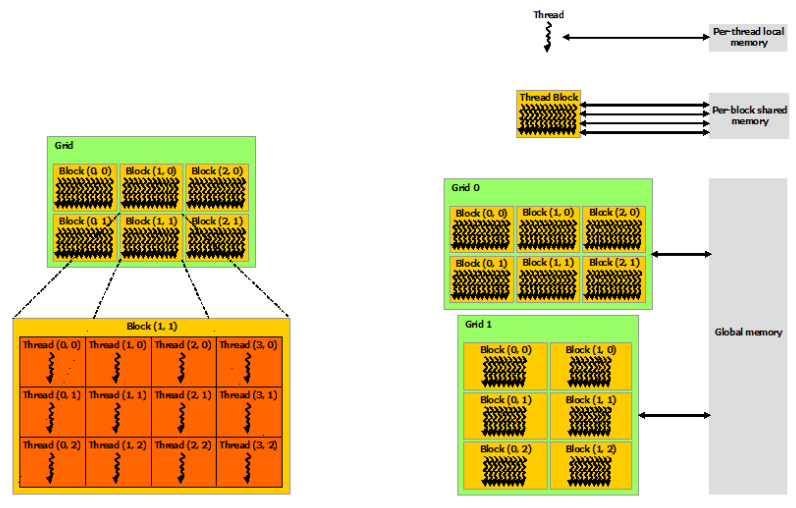
\includegraphics[height=.7\textheight]{./cudaorg.png}
	\newline
	\textbf{Credit: CUDA C Programming Guide}
	\end{figure}
\end{frame}
% END CUDA INTRO

% BEGIN PAR RADIUS
\begin{frame}
\frametitle{Parallel Radius Finding: Translating}
Back to parallel Roughsort: we know we can find the radius in parallel.  Merely need to convert the pseudocode to CUDA code.
\newline\newline
Straightforward for $LR$ list, slightly less so for $RL$, least straightforward for $DM$.
\newline\newline
Eventually settled on a $DM$ list determination based on the sequential, with array indices fixed to thread ID.
\newline\newline
Added an efficient method to check for full array sortedness as part of the $RL$ and $LR$ list components.
\end{frame}


\begin{frame}
	\frametitle{Parallel Radius Finding: Scaling Up}
Testing:
\begin{enumerate}
	\item Worked fine for a low values
	\item Did not function at all for large values of $n$ (widely inaccurate $k$ values)
\end{enumerate}
\end{frame}

\begin{frame}
	\frametitle{Parallel Radius Finding: Re-Visiting}
	Cause/Fix:
	\begin{enumerate}
		\item Asked individual threads to allocate their slot in the global memory $RL$ and $LR$ lists upon startup
		\item Not all threads are immediately scheduled for large thread counts--bug
		\item Subsequently started copying all values before kernel launch
	\end{enumerate}
	
\end{frame}

\begin{frame}
	\frametitle{Parallel Radius Finding: Scaling Up (2)}
	After fixing, $DM$ list was correct to an extent, but it was slow.
	\newline\newline
	Resolved this by realizing only need our "radius" to approximate the real $k$ value, in that we just need the next power of two greater
	\newline\newline
	Added \texttt{Thrust max_element} code to find the greatest value in the $DM$ list, thus yielding our radius
\end{frame}
% END PAR RADIUS

% BEGIN PAR RADIUS RESULTS
\begin{frame}
\frametitle{Parallel Radius Finding: Results ($k = 2$)}
\begin{figure}
\resizebox{!}{.8\textheight}{% GNUPLOT: LaTeX picture
\setlength{\unitlength}{0.240900pt}
\ifx\plotpoint\undefined\newsavebox{\plotpoint}\fi
\sbox{\plotpoint}{\rule[-0.200pt]{0.400pt}{0.400pt}}%
\begin{picture}(2550,1800)(0,0)
\sbox{\plotpoint}{\rule[-0.200pt]{0.400pt}{0.400pt}}%
\put(131.0,131.0){\rule[-0.200pt]{4.818pt}{0.400pt}}
\put(111,131){\makebox(0,0)[r]{$0$}}
\put(2469.0,131.0){\rule[-0.200pt]{4.818pt}{0.400pt}}
\put(131.0,364.0){\rule[-0.200pt]{4.818pt}{0.400pt}}
\put(111,364){\makebox(0,0)[r]{$2$}}
\put(2469.0,364.0){\rule[-0.200pt]{4.818pt}{0.400pt}}
\put(131.0,596.0){\rule[-0.200pt]{4.818pt}{0.400pt}}
\put(111,596){\makebox(0,0)[r]{$4$}}
\put(2469.0,596.0){\rule[-0.200pt]{4.818pt}{0.400pt}}
\put(131.0,829.0){\rule[-0.200pt]{4.818pt}{0.400pt}}
\put(111,829){\makebox(0,0)[r]{$6$}}
\put(2469.0,829.0){\rule[-0.200pt]{4.818pt}{0.400pt}}
\put(131.0,1061.0){\rule[-0.200pt]{4.818pt}{0.400pt}}
\put(111,1061){\makebox(0,0)[r]{$8$}}
\put(2469.0,1061.0){\rule[-0.200pt]{4.818pt}{0.400pt}}
\put(131.0,1294.0){\rule[-0.200pt]{4.818pt}{0.400pt}}
\put(111,1294){\makebox(0,0)[r]{$10$}}
\put(2469.0,1294.0){\rule[-0.200pt]{4.818pt}{0.400pt}}
\put(131.0,1526.0){\rule[-0.200pt]{4.818pt}{0.400pt}}
\put(111,1526){\makebox(0,0)[r]{$12$}}
\put(2469.0,1526.0){\rule[-0.200pt]{4.818pt}{0.400pt}}
\put(131.0,1759.0){\rule[-0.200pt]{4.818pt}{0.400pt}}
\put(111,1759){\makebox(0,0)[r]{$14$}}
\put(2469.0,1759.0){\rule[-0.200pt]{4.818pt}{0.400pt}}
\put(131.0,131.0){\rule[-0.200pt]{0.400pt}{4.818pt}}
\put(131,90){\makebox(0,0){.025}}
\put(131.0,1739.0){\rule[-0.200pt]{0.400pt}{4.818pt}}
\put(215.0,131.0){\rule[-0.200pt]{0.400pt}{4.818pt}}
\put(215,90){\makebox(0,0){.05}}
\put(215.0,1739.0){\rule[-0.200pt]{0.400pt}{4.818pt}}
\put(299.0,131.0){\rule[-0.200pt]{0.400pt}{4.818pt}}
\put(299,90){\makebox(0,0){.075}}
\put(299.0,1739.0){\rule[-0.200pt]{0.400pt}{4.818pt}}
\put(384.0,131.0){\rule[-0.200pt]{0.400pt}{4.818pt}}
\put(384,90){\makebox(0,0){.1}}
\put(384.0,1739.0){\rule[-0.200pt]{0.400pt}{4.818pt}}
\put(468.0,131.0){\rule[-0.200pt]{0.400pt}{4.818pt}}
\put(468,90){\makebox(0,0){.125}}
\put(468.0,1739.0){\rule[-0.200pt]{0.400pt}{4.818pt}}
\put(552.0,131.0){\rule[-0.200pt]{0.400pt}{4.818pt}}
\put(552,90){\makebox(0,0){.15}}
\put(552.0,1739.0){\rule[-0.200pt]{0.400pt}{4.818pt}}
\put(636.0,131.0){\rule[-0.200pt]{0.400pt}{4.818pt}}
\put(636,90){\makebox(0,0){.175}}
\put(636.0,1739.0){\rule[-0.200pt]{0.400pt}{4.818pt}}
\put(721.0,131.0){\rule[-0.200pt]{0.400pt}{4.818pt}}
\put(721,90){\makebox(0,0){.2}}
\put(721.0,1739.0){\rule[-0.200pt]{0.400pt}{4.818pt}}
\put(805.0,131.0){\rule[-0.200pt]{0.400pt}{4.818pt}}
\put(805,90){\makebox(0,0){.25}}
\put(805.0,1739.0){\rule[-0.200pt]{0.400pt}{4.818pt}}
\put(889.0,131.0){\rule[-0.200pt]{0.400pt}{4.818pt}}
\put(889,90){\makebox(0,0){.3}}
\put(889.0,1739.0){\rule[-0.200pt]{0.400pt}{4.818pt}}
\put(973.0,131.0){\rule[-0.200pt]{0.400pt}{4.818pt}}
\put(973,90){\makebox(0,0){.35}}
\put(973.0,1739.0){\rule[-0.200pt]{0.400pt}{4.818pt}}
\put(1057.0,131.0){\rule[-0.200pt]{0.400pt}{4.818pt}}
\put(1057,90){\makebox(0,0){.4}}
\put(1057.0,1739.0){\rule[-0.200pt]{0.400pt}{4.818pt}}
\put(1142.0,131.0){\rule[-0.200pt]{0.400pt}{4.818pt}}
\put(1142,90){\makebox(0,0){.45}}
\put(1142.0,1739.0){\rule[-0.200pt]{0.400pt}{4.818pt}}
\put(1226.0,131.0){\rule[-0.200pt]{0.400pt}{4.818pt}}
\put(1226,90){\makebox(0,0){.5}}
\put(1226.0,1739.0){\rule[-0.200pt]{0.400pt}{4.818pt}}
\put(1310.0,131.0){\rule[-0.200pt]{0.400pt}{4.818pt}}
\put(1310,90){\makebox(0,0){.6}}
\put(1310.0,1739.0){\rule[-0.200pt]{0.400pt}{4.818pt}}
\put(1394.0,131.0){\rule[-0.200pt]{0.400pt}{4.818pt}}
\put(1394,90){\makebox(0,0){.7}}
\put(1394.0,1739.0){\rule[-0.200pt]{0.400pt}{4.818pt}}
\put(1478.0,131.0){\rule[-0.200pt]{0.400pt}{4.818pt}}
\put(1478,90){\makebox(0,0){.8}}
\put(1478.0,1739.0){\rule[-0.200pt]{0.400pt}{4.818pt}}
\put(1563.0,131.0){\rule[-0.200pt]{0.400pt}{4.818pt}}
\put(1563,90){\makebox(0,0){.9}}
\put(1563.0,1739.0){\rule[-0.200pt]{0.400pt}{4.818pt}}
\put(1647.0,131.0){\rule[-0.200pt]{0.400pt}{4.818pt}}
\put(1647,90){\makebox(0,0){1}}
\put(1647.0,1739.0){\rule[-0.200pt]{0.400pt}{4.818pt}}
\put(1731.0,131.0){\rule[-0.200pt]{0.400pt}{4.818pt}}
\put(1731,90){\makebox(0,0){1.1}}
\put(1731.0,1739.0){\rule[-0.200pt]{0.400pt}{4.818pt}}
\put(1815.0,131.0){\rule[-0.200pt]{0.400pt}{4.818pt}}
\put(1815,90){\makebox(0,0){1.2}}
\put(1815.0,1739.0){\rule[-0.200pt]{0.400pt}{4.818pt}}
\put(1899.0,131.0){\rule[-0.200pt]{0.400pt}{4.818pt}}
\put(1899,90){\makebox(0,0){1.3}}
\put(1899.0,1739.0){\rule[-0.200pt]{0.400pt}{4.818pt}}
\put(1984.0,131.0){\rule[-0.200pt]{0.400pt}{4.818pt}}
\put(1984,90){\makebox(0,0){1.4}}
\put(1984.0,1739.0){\rule[-0.200pt]{0.400pt}{4.818pt}}
\put(2068.0,131.0){\rule[-0.200pt]{0.400pt}{4.818pt}}
\put(2068,90){\makebox(0,0){1.5}}
\put(2068.0,1739.0){\rule[-0.200pt]{0.400pt}{4.818pt}}
\put(2152.0,131.0){\rule[-0.200pt]{0.400pt}{4.818pt}}
\put(2152,90){\makebox(0,0){1.6}}
\put(2152.0,1739.0){\rule[-0.200pt]{0.400pt}{4.818pt}}
\put(2236.0,131.0){\rule[-0.200pt]{0.400pt}{4.818pt}}
\put(2236,90){\makebox(0,0){1.7}}
\put(2236.0,1739.0){\rule[-0.200pt]{0.400pt}{4.818pt}}
\put(2321.0,131.0){\rule[-0.200pt]{0.400pt}{4.818pt}}
\put(2321,90){\makebox(0,0){1.8}}
\put(2321.0,1739.0){\rule[-0.200pt]{0.400pt}{4.818pt}}
\put(2405.0,131.0){\rule[-0.200pt]{0.400pt}{4.818pt}}
\put(2405,90){\makebox(0,0){1.9}}
\put(2405.0,1739.0){\rule[-0.200pt]{0.400pt}{4.818pt}}
\put(2489.0,131.0){\rule[-0.200pt]{0.400pt}{4.818pt}}
\put(2489,90){\makebox(0,0){2}}
\put(2489.0,1739.0){\rule[-0.200pt]{0.400pt}{4.818pt}}
\put(131.0,131.0){\rule[-0.200pt]{0.400pt}{392.185pt}}
\put(131.0,131.0){\rule[-0.200pt]{568.042pt}{0.400pt}}
\put(2489.0,131.0){\rule[-0.200pt]{0.400pt}{392.185pt}}
\put(131.0,1759.0){\rule[-0.200pt]{568.042pt}{0.400pt}}
\put(30,945){\makebox(0,0){(ms)}}
\put(1310,29){\makebox(0,0){$n$}}
\put(431,1708){\makebox(0,0)[r]{   Seq. Radius}}
\put(451.0,1708.0){\rule[-0.200pt]{24.090pt}{0.400pt}}
\put(131,131){\usebox{\plotpoint}}
\multiput(468.58,131.00)(0.499,0.691){165}{\rule{0.120pt}{0.652pt}}
\multiput(467.17,131.00)(84.000,114.646){2}{\rule{0.400pt}{0.326pt}}
\put(131.0,131.0){\rule[-0.200pt]{81.183pt}{0.400pt}}
\multiput(805.58,247.00)(0.499,0.697){165}{\rule{0.120pt}{0.657pt}}
\multiput(804.17,247.00)(84.000,115.636){2}{\rule{0.400pt}{0.329pt}}
\put(552.0,247.0){\rule[-0.200pt]{60.948pt}{0.400pt}}
\multiput(1057.58,364.00)(0.499,0.683){167}{\rule{0.120pt}{0.646pt}}
\multiput(1056.17,364.00)(85.000,114.659){2}{\rule{0.400pt}{0.323pt}}
\put(889.0,364.0){\rule[-0.200pt]{40.471pt}{0.400pt}}
\multiput(1226.58,480.00)(0.499,0.691){165}{\rule{0.120pt}{0.652pt}}
\multiput(1225.17,480.00)(84.000,114.646){2}{\rule{0.400pt}{0.326pt}}
\put(1142.0,480.0){\rule[-0.200pt]{20.236pt}{0.400pt}}
\multiput(1394.58,596.00)(0.499,0.691){165}{\rule{0.120pt}{0.652pt}}
\multiput(1393.17,596.00)(84.000,114.646){2}{\rule{0.400pt}{0.326pt}}
\multiput(1478.58,712.00)(0.499,0.689){167}{\rule{0.120pt}{0.651pt}}
\multiput(1477.17,712.00)(85.000,115.650){2}{\rule{0.400pt}{0.325pt}}
\multiput(1563.58,829.00)(0.499,0.691){165}{\rule{0.120pt}{0.652pt}}
\multiput(1562.17,829.00)(84.000,114.646){2}{\rule{0.400pt}{0.326pt}}
\put(1310.0,596.0){\rule[-0.200pt]{20.236pt}{0.400pt}}
\multiput(1731.58,945.00)(0.499,0.691){165}{\rule{0.120pt}{0.652pt}}
\multiput(1730.17,945.00)(84.000,114.646){2}{\rule{0.400pt}{0.326pt}}
\multiput(1815.58,1061.00)(0.499,0.697){165}{\rule{0.120pt}{0.657pt}}
\multiput(1814.17,1061.00)(84.000,115.636){2}{\rule{0.400pt}{0.329pt}}
\put(1647.0,945.0){\rule[-0.200pt]{20.236pt}{0.400pt}}
\multiput(1984.58,1178.00)(0.499,0.691){165}{\rule{0.120pt}{0.652pt}}
\multiput(1983.17,1178.00)(84.000,114.646){2}{\rule{0.400pt}{0.326pt}}
\multiput(2068.58,1294.00)(0.499,0.691){165}{\rule{0.120pt}{0.652pt}}
\multiput(2067.17,1294.00)(84.000,114.646){2}{\rule{0.400pt}{0.326pt}}
\put(1899.0,1178.0){\rule[-0.200pt]{20.476pt}{0.400pt}}
\multiput(2236.58,1410.00)(0.499,0.683){167}{\rule{0.120pt}{0.646pt}}
\multiput(2235.17,1410.00)(85.000,114.659){2}{\rule{0.400pt}{0.323pt}}
\multiput(2321.58,1526.00)(0.499,0.697){165}{\rule{0.120pt}{0.657pt}}
\multiput(2320.17,1526.00)(84.000,115.636){2}{\rule{0.400pt}{0.329pt}}
\multiput(2405.58,1643.00)(0.499,0.691){165}{\rule{0.120pt}{0.652pt}}
\multiput(2404.17,1643.00)(84.000,114.646){2}{\rule{0.400pt}{0.326pt}}
\put(131,131){\makebox(0,0){$\bullet$}}
\put(215,131){\makebox(0,0){$\bullet$}}
\put(299,131){\makebox(0,0){$\bullet$}}
\put(384,131){\makebox(0,0){$\bullet$}}
\put(468,131){\makebox(0,0){$\bullet$}}
\put(552,247){\makebox(0,0){$\bullet$}}
\put(636,247){\makebox(0,0){$\bullet$}}
\put(721,247){\makebox(0,0){$\bullet$}}
\put(805,247){\makebox(0,0){$\bullet$}}
\put(889,364){\makebox(0,0){$\bullet$}}
\put(973,364){\makebox(0,0){$\bullet$}}
\put(1057,364){\makebox(0,0){$\bullet$}}
\put(1142,480){\makebox(0,0){$\bullet$}}
\put(1226,480){\makebox(0,0){$\bullet$}}
\put(1310,596){\makebox(0,0){$\bullet$}}
\put(1394,596){\makebox(0,0){$\bullet$}}
\put(1478,712){\makebox(0,0){$\bullet$}}
\put(1563,829){\makebox(0,0){$\bullet$}}
\put(1647,945){\makebox(0,0){$\bullet$}}
\put(1731,945){\makebox(0,0){$\bullet$}}
\put(1815,1061){\makebox(0,0){$\bullet$}}
\put(1899,1178){\makebox(0,0){$\bullet$}}
\put(1984,1178){\makebox(0,0){$\bullet$}}
\put(2068,1294){\makebox(0,0){$\bullet$}}
\put(2152,1410){\makebox(0,0){$\bullet$}}
\put(2236,1410){\makebox(0,0){$\bullet$}}
\put(2321,1526){\makebox(0,0){$\bullet$}}
\put(2405,1643){\makebox(0,0){$\bullet$}}
\put(2489,1759){\makebox(0,0){$\bullet$}}
\put(501,1708){\makebox(0,0){$\bullet$}}
\put(2152.0,1410.0){\rule[-0.200pt]{20.236pt}{0.400pt}}
\put(431,1646){\makebox(0,0)[r]{   Par. Radius}}
\put(451.0,1646.0){\rule[-0.200pt]{24.090pt}{0.400pt}}
\put(131,131){\usebox{\plotpoint}}
\multiput(215.58,131.00)(0.499,0.691){165}{\rule{0.120pt}{0.652pt}}
\multiput(214.17,131.00)(84.000,114.646){2}{\rule{0.400pt}{0.326pt}}
\put(131.0,131.0){\rule[-0.200pt]{20.236pt}{0.400pt}}
\multiput(805.58,247.00)(0.499,0.697){165}{\rule{0.120pt}{0.657pt}}
\multiput(804.17,247.00)(84.000,115.636){2}{\rule{0.400pt}{0.329pt}}
\put(299.0,247.0){\rule[-0.200pt]{121.895pt}{0.400pt}}
\multiput(1142.58,364.00)(0.499,0.691){165}{\rule{0.120pt}{0.652pt}}
\multiput(1141.17,364.00)(84.000,114.646){2}{\rule{0.400pt}{0.326pt}}
\put(889.0,364.0){\rule[-0.200pt]{60.948pt}{0.400pt}}
\multiput(1310.58,480.00)(0.499,0.691){165}{\rule{0.120pt}{0.652pt}}
\multiput(1309.17,480.00)(84.000,114.646){2}{\rule{0.400pt}{0.326pt}}
\put(1226.0,480.0){\rule[-0.200pt]{20.236pt}{0.400pt}}
\multiput(1478.58,596.00)(0.499,0.683){167}{\rule{0.120pt}{0.646pt}}
\multiput(1477.17,596.00)(85.000,114.659){2}{\rule{0.400pt}{0.323pt}}
\put(1394.0,596.0){\rule[-0.200pt]{20.236pt}{0.400pt}}
\multiput(1647.58,712.00)(0.499,0.697){165}{\rule{0.120pt}{0.657pt}}
\multiput(1646.17,712.00)(84.000,115.636){2}{\rule{0.400pt}{0.329pt}}
\multiput(1731.58,829.00)(0.499,0.691){165}{\rule{0.120pt}{0.652pt}}
\multiput(1730.17,829.00)(84.000,114.646){2}{\rule{0.400pt}{0.326pt}}
\put(1563.0,712.0){\rule[-0.200pt]{20.236pt}{0.400pt}}
\multiput(1899.58,945.00)(0.499,0.683){167}{\rule{0.120pt}{0.646pt}}
\multiput(1898.17,945.00)(85.000,114.659){2}{\rule{0.400pt}{0.323pt}}
\put(1815.0,945.0){\rule[-0.200pt]{20.236pt}{0.400pt}}
\multiput(2068.58,1061.00)(0.499,0.697){165}{\rule{0.120pt}{0.657pt}}
\multiput(2067.17,1061.00)(84.000,115.636){2}{\rule{0.400pt}{0.329pt}}
\put(1984.0,1061.0){\rule[-0.200pt]{20.236pt}{0.400pt}}
\multiput(2236.58,1178.00)(0.499,0.683){167}{\rule{0.120pt}{0.646pt}}
\multiput(2235.17,1178.00)(85.000,114.659){2}{\rule{0.400pt}{0.323pt}}
\put(2152.0,1178.0){\rule[-0.200pt]{20.236pt}{0.400pt}}
\multiput(2405.58,1294.00)(0.499,0.691){165}{\rule{0.120pt}{0.652pt}}
\multiput(2404.17,1294.00)(84.000,114.646){2}{\rule{0.400pt}{0.326pt}}
\put(131,131){\makebox(0,0){$\circ$}}
\put(215,131){\makebox(0,0){$\circ$}}
\put(299,247){\makebox(0,0){$\circ$}}
\put(384,247){\makebox(0,0){$\circ$}}
\put(468,247){\makebox(0,0){$\circ$}}
\put(552,247){\makebox(0,0){$\circ$}}
\put(636,247){\makebox(0,0){$\circ$}}
\put(721,247){\makebox(0,0){$\circ$}}
\put(805,247){\makebox(0,0){$\circ$}}
\put(889,364){\makebox(0,0){$\circ$}}
\put(973,364){\makebox(0,0){$\circ$}}
\put(1057,364){\makebox(0,0){$\circ$}}
\put(1142,364){\makebox(0,0){$\circ$}}
\put(1226,480){\makebox(0,0){$\circ$}}
\put(1310,480){\makebox(0,0){$\circ$}}
\put(1394,596){\makebox(0,0){$\circ$}}
\put(1478,596){\makebox(0,0){$\circ$}}
\put(1563,712){\makebox(0,0){$\circ$}}
\put(1647,712){\makebox(0,0){$\circ$}}
\put(1731,829){\makebox(0,0){$\circ$}}
\put(1815,945){\makebox(0,0){$\circ$}}
\put(1899,945){\makebox(0,0){$\circ$}}
\put(1984,1061){\makebox(0,0){$\circ$}}
\put(2068,1061){\makebox(0,0){$\circ$}}
\put(2152,1178){\makebox(0,0){$\circ$}}
\put(2236,1178){\makebox(0,0){$\circ$}}
\put(2321,1294){\makebox(0,0){$\circ$}}
\put(2405,1294){\makebox(0,0){$\circ$}}
\put(2489,1410){\makebox(0,0){$\circ$}}
\put(501,1646){\makebox(0,0){$\circ$}}
\put(2321.0,1294.0){\rule[-0.200pt]{20.236pt}{0.400pt}}
\put(131.0,131.0){\rule[-0.200pt]{0.400pt}{392.185pt}}
\put(131.0,131.0){\rule[-0.200pt]{568.042pt}{0.400pt}}
\put(2489.0,131.0){\rule[-0.200pt]{0.400pt}{392.185pt}}
\put(131.0,1759.0){\rule[-0.200pt]{568.042pt}{0.400pt}}
\end{picture}
}
\end{figure}
\end{frame}

\begin{frame}
\frametitle{Parallel Radius Finding: Results($k = 100$)}
\begin{figure}
	\resizebox{!}{.8\textheight}{% GNUPLOT: LaTeX picture
\setlength{\unitlength}{0.240900pt}
\ifx\plotpoint\undefined\newsavebox{\plotpoint}\fi
\sbox{\plotpoint}{\rule[-0.200pt]{0.400pt}{0.400pt}}%
\begin{picture}(2550,1800)(0,0)
\sbox{\plotpoint}{\rule[-0.200pt]{0.400pt}{0.400pt}}%
\put(131.0,131.0){\rule[-0.200pt]{4.818pt}{0.400pt}}
\put(111,131){\makebox(0,0)[r]{$0$}}
\put(2469.0,131.0){\rule[-0.200pt]{4.818pt}{0.400pt}}
\put(131.0,335.0){\rule[-0.200pt]{4.818pt}{0.400pt}}
\put(111,335){\makebox(0,0)[r]{$2$}}
\put(2469.0,335.0){\rule[-0.200pt]{4.818pt}{0.400pt}}
\put(131.0,538.0){\rule[-0.200pt]{4.818pt}{0.400pt}}
\put(111,538){\makebox(0,0)[r]{$4$}}
\put(2469.0,538.0){\rule[-0.200pt]{4.818pt}{0.400pt}}
\put(131.0,742.0){\rule[-0.200pt]{4.818pt}{0.400pt}}
\put(111,742){\makebox(0,0)[r]{$6$}}
\put(2469.0,742.0){\rule[-0.200pt]{4.818pt}{0.400pt}}
\put(131.0,945.0){\rule[-0.200pt]{4.818pt}{0.400pt}}
\put(111,945){\makebox(0,0)[r]{$8$}}
\put(2469.0,945.0){\rule[-0.200pt]{4.818pt}{0.400pt}}
\put(131.0,1149.0){\rule[-0.200pt]{4.818pt}{0.400pt}}
\put(111,1149){\makebox(0,0)[r]{$10$}}
\put(2469.0,1149.0){\rule[-0.200pt]{4.818pt}{0.400pt}}
\put(131.0,1352.0){\rule[-0.200pt]{4.818pt}{0.400pt}}
\put(111,1352){\makebox(0,0)[r]{$12$}}
\put(2469.0,1352.0){\rule[-0.200pt]{4.818pt}{0.400pt}}
\put(131.0,1556.0){\rule[-0.200pt]{4.818pt}{0.400pt}}
\put(111,1556){\makebox(0,0)[r]{$14$}}
\put(2469.0,1556.0){\rule[-0.200pt]{4.818pt}{0.400pt}}
\put(131.0,1759.0){\rule[-0.200pt]{4.818pt}{0.400pt}}
\put(111,1759){\makebox(0,0)[r]{$16$}}
\put(2469.0,1759.0){\rule[-0.200pt]{4.818pt}{0.400pt}}
\put(131.0,131.0){\rule[-0.200pt]{0.400pt}{4.818pt}}
\put(131,90){\makebox(0,0){.025}}
\put(131.0,1739.0){\rule[-0.200pt]{0.400pt}{4.818pt}}
\put(215.0,131.0){\rule[-0.200pt]{0.400pt}{4.818pt}}
\put(215,90){\makebox(0,0){.05}}
\put(215.0,1739.0){\rule[-0.200pt]{0.400pt}{4.818pt}}
\put(299.0,131.0){\rule[-0.200pt]{0.400pt}{4.818pt}}
\put(299,90){\makebox(0,0){.075}}
\put(299.0,1739.0){\rule[-0.200pt]{0.400pt}{4.818pt}}
\put(384.0,131.0){\rule[-0.200pt]{0.400pt}{4.818pt}}
\put(384,90){\makebox(0,0){.1}}
\put(384.0,1739.0){\rule[-0.200pt]{0.400pt}{4.818pt}}
\put(468.0,131.0){\rule[-0.200pt]{0.400pt}{4.818pt}}
\put(468,90){\makebox(0,0){.125}}
\put(468.0,1739.0){\rule[-0.200pt]{0.400pt}{4.818pt}}
\put(552.0,131.0){\rule[-0.200pt]{0.400pt}{4.818pt}}
\put(552,90){\makebox(0,0){.15}}
\put(552.0,1739.0){\rule[-0.200pt]{0.400pt}{4.818pt}}
\put(636.0,131.0){\rule[-0.200pt]{0.400pt}{4.818pt}}
\put(636,90){\makebox(0,0){.175}}
\put(636.0,1739.0){\rule[-0.200pt]{0.400pt}{4.818pt}}
\put(721.0,131.0){\rule[-0.200pt]{0.400pt}{4.818pt}}
\put(721,90){\makebox(0,0){.2}}
\put(721.0,1739.0){\rule[-0.200pt]{0.400pt}{4.818pt}}
\put(805.0,131.0){\rule[-0.200pt]{0.400pt}{4.818pt}}
\put(805,90){\makebox(0,0){.25}}
\put(805.0,1739.0){\rule[-0.200pt]{0.400pt}{4.818pt}}
\put(889.0,131.0){\rule[-0.200pt]{0.400pt}{4.818pt}}
\put(889,90){\makebox(0,0){.3}}
\put(889.0,1739.0){\rule[-0.200pt]{0.400pt}{4.818pt}}
\put(973.0,131.0){\rule[-0.200pt]{0.400pt}{4.818pt}}
\put(973,90){\makebox(0,0){.35}}
\put(973.0,1739.0){\rule[-0.200pt]{0.400pt}{4.818pt}}
\put(1057.0,131.0){\rule[-0.200pt]{0.400pt}{4.818pt}}
\put(1057,90){\makebox(0,0){.4}}
\put(1057.0,1739.0){\rule[-0.200pt]{0.400pt}{4.818pt}}
\put(1142.0,131.0){\rule[-0.200pt]{0.400pt}{4.818pt}}
\put(1142,90){\makebox(0,0){.45}}
\put(1142.0,1739.0){\rule[-0.200pt]{0.400pt}{4.818pt}}
\put(1226.0,131.0){\rule[-0.200pt]{0.400pt}{4.818pt}}
\put(1226,90){\makebox(0,0){.5}}
\put(1226.0,1739.0){\rule[-0.200pt]{0.400pt}{4.818pt}}
\put(1310.0,131.0){\rule[-0.200pt]{0.400pt}{4.818pt}}
\put(1310,90){\makebox(0,0){.6}}
\put(1310.0,1739.0){\rule[-0.200pt]{0.400pt}{4.818pt}}
\put(1394.0,131.0){\rule[-0.200pt]{0.400pt}{4.818pt}}
\put(1394,90){\makebox(0,0){.7}}
\put(1394.0,1739.0){\rule[-0.200pt]{0.400pt}{4.818pt}}
\put(1478.0,131.0){\rule[-0.200pt]{0.400pt}{4.818pt}}
\put(1478,90){\makebox(0,0){.8}}
\put(1478.0,1739.0){\rule[-0.200pt]{0.400pt}{4.818pt}}
\put(1563.0,131.0){\rule[-0.200pt]{0.400pt}{4.818pt}}
\put(1563,90){\makebox(0,0){.9}}
\put(1563.0,1739.0){\rule[-0.200pt]{0.400pt}{4.818pt}}
\put(1647.0,131.0){\rule[-0.200pt]{0.400pt}{4.818pt}}
\put(1647,90){\makebox(0,0){1}}
\put(1647.0,1739.0){\rule[-0.200pt]{0.400pt}{4.818pt}}
\put(1731.0,131.0){\rule[-0.200pt]{0.400pt}{4.818pt}}
\put(1731,90){\makebox(0,0){1.1}}
\put(1731.0,1739.0){\rule[-0.200pt]{0.400pt}{4.818pt}}
\put(1815.0,131.0){\rule[-0.200pt]{0.400pt}{4.818pt}}
\put(1815,90){\makebox(0,0){1.2}}
\put(1815.0,1739.0){\rule[-0.200pt]{0.400pt}{4.818pt}}
\put(1899.0,131.0){\rule[-0.200pt]{0.400pt}{4.818pt}}
\put(1899,90){\makebox(0,0){1.3}}
\put(1899.0,1739.0){\rule[-0.200pt]{0.400pt}{4.818pt}}
\put(1984.0,131.0){\rule[-0.200pt]{0.400pt}{4.818pt}}
\put(1984,90){\makebox(0,0){1.4}}
\put(1984.0,1739.0){\rule[-0.200pt]{0.400pt}{4.818pt}}
\put(2068.0,131.0){\rule[-0.200pt]{0.400pt}{4.818pt}}
\put(2068,90){\makebox(0,0){1.5}}
\put(2068.0,1739.0){\rule[-0.200pt]{0.400pt}{4.818pt}}
\put(2152.0,131.0){\rule[-0.200pt]{0.400pt}{4.818pt}}
\put(2152,90){\makebox(0,0){1.6}}
\put(2152.0,1739.0){\rule[-0.200pt]{0.400pt}{4.818pt}}
\put(2236.0,131.0){\rule[-0.200pt]{0.400pt}{4.818pt}}
\put(2236,90){\makebox(0,0){1.7}}
\put(2236.0,1739.0){\rule[-0.200pt]{0.400pt}{4.818pt}}
\put(2321.0,131.0){\rule[-0.200pt]{0.400pt}{4.818pt}}
\put(2321,90){\makebox(0,0){1.8}}
\put(2321.0,1739.0){\rule[-0.200pt]{0.400pt}{4.818pt}}
\put(2405.0,131.0){\rule[-0.200pt]{0.400pt}{4.818pt}}
\put(2405,90){\makebox(0,0){1.9}}
\put(2405.0,1739.0){\rule[-0.200pt]{0.400pt}{4.818pt}}
\put(2489.0,131.0){\rule[-0.200pt]{0.400pt}{4.818pt}}
\put(2489,90){\makebox(0,0){2}}
\put(2489.0,1739.0){\rule[-0.200pt]{0.400pt}{4.818pt}}
\put(131.0,131.0){\rule[-0.200pt]{0.400pt}{392.185pt}}
\put(131.0,131.0){\rule[-0.200pt]{568.042pt}{0.400pt}}
\put(2489.0,131.0){\rule[-0.200pt]{0.400pt}{392.185pt}}
\put(131.0,1759.0){\rule[-0.200pt]{568.042pt}{0.400pt}}
\put(30,945){\makebox(0,0){(ms)}}
\put(1310,29){\makebox(0,0){$n$}}
\put(431,1708){\makebox(0,0)[r]{   Seq. Radius}}
\put(451.0,1708.0){\rule[-0.200pt]{24.090pt}{0.400pt}}
\put(131,131){\usebox{\plotpoint}}
\multiput(552.58,131.00)(0.499,0.607){165}{\rule{0.120pt}{0.586pt}}
\multiput(551.17,131.00)(84.000,100.784){2}{\rule{0.400pt}{0.293pt}}
\put(131.0,131.0){\rule[-0.200pt]{101.419pt}{0.400pt}}
\multiput(889.58,233.00)(0.499,0.607){165}{\rule{0.120pt}{0.586pt}}
\multiput(888.17,233.00)(84.000,100.784){2}{\rule{0.400pt}{0.293pt}}
\put(636.0,233.0){\rule[-0.200pt]{60.948pt}{0.400pt}}
\multiput(1226.58,335.00)(0.499,0.601){165}{\rule{0.120pt}{0.581pt}}
\multiput(1225.17,335.00)(84.000,99.794){2}{\rule{0.400pt}{0.290pt}}
\put(973.0,335.0){\rule[-0.200pt]{60.948pt}{0.400pt}}
\multiput(1394.58,436.00)(0.499,0.607){165}{\rule{0.120pt}{0.586pt}}
\multiput(1393.17,436.00)(84.000,100.784){2}{\rule{0.400pt}{0.293pt}}
\put(1310.0,436.0){\rule[-0.200pt]{20.236pt}{0.400pt}}
\multiput(1563.58,538.00)(0.499,0.607){165}{\rule{0.120pt}{0.586pt}}
\multiput(1562.17,538.00)(84.000,100.784){2}{\rule{0.400pt}{0.293pt}}
\multiput(1647.58,640.00)(0.499,0.607){165}{\rule{0.120pt}{0.586pt}}
\multiput(1646.17,640.00)(84.000,100.784){2}{\rule{0.400pt}{0.293pt}}
\put(1478.0,538.0){\rule[-0.200pt]{20.476pt}{0.400pt}}
\multiput(1815.58,742.00)(0.499,0.601){165}{\rule{0.120pt}{0.581pt}}
\multiput(1814.17,742.00)(84.000,99.794){2}{\rule{0.400pt}{0.290pt}}
\put(1731.0,742.0){\rule[-0.200pt]{20.236pt}{0.400pt}}
\multiput(1984.58,843.00)(0.499,0.607){165}{\rule{0.120pt}{0.586pt}}
\multiput(1983.17,843.00)(84.000,100.784){2}{\rule{0.400pt}{0.293pt}}
\put(1899.0,843.0){\rule[-0.200pt]{20.476pt}{0.400pt}}
\multiput(2152.58,945.00)(0.499,0.607){165}{\rule{0.120pt}{0.586pt}}
\multiput(2151.17,945.00)(84.000,100.784){2}{\rule{0.400pt}{0.293pt}}
\put(2068.0,945.0){\rule[-0.200pt]{20.236pt}{0.400pt}}
\multiput(2321.58,1047.00)(0.499,0.607){165}{\rule{0.120pt}{0.586pt}}
\multiput(2320.17,1047.00)(84.000,100.784){2}{\rule{0.400pt}{0.293pt}}
\multiput(2405.58,1149.00)(0.499,0.601){165}{\rule{0.120pt}{0.581pt}}
\multiput(2404.17,1149.00)(84.000,99.794){2}{\rule{0.400pt}{0.290pt}}
\put(131,131){\makebox(0,0){$\bullet$}}
\put(215,131){\makebox(0,0){$\bullet$}}
\put(299,131){\makebox(0,0){$\bullet$}}
\put(384,131){\makebox(0,0){$\bullet$}}
\put(468,131){\makebox(0,0){$\bullet$}}
\put(552,131){\makebox(0,0){$\bullet$}}
\put(636,233){\makebox(0,0){$\bullet$}}
\put(721,233){\makebox(0,0){$\bullet$}}
\put(805,233){\makebox(0,0){$\bullet$}}
\put(889,233){\makebox(0,0){$\bullet$}}
\put(973,335){\makebox(0,0){$\bullet$}}
\put(1057,335){\makebox(0,0){$\bullet$}}
\put(1142,335){\makebox(0,0){$\bullet$}}
\put(1226,335){\makebox(0,0){$\bullet$}}
\put(1310,436){\makebox(0,0){$\bullet$}}
\put(1394,436){\makebox(0,0){$\bullet$}}
\put(1478,538){\makebox(0,0){$\bullet$}}
\put(1563,538){\makebox(0,0){$\bullet$}}
\put(1647,640){\makebox(0,0){$\bullet$}}
\put(1731,742){\makebox(0,0){$\bullet$}}
\put(1815,742){\makebox(0,0){$\bullet$}}
\put(1899,843){\makebox(0,0){$\bullet$}}
\put(1984,843){\makebox(0,0){$\bullet$}}
\put(2068,945){\makebox(0,0){$\bullet$}}
\put(2152,945){\makebox(0,0){$\bullet$}}
\put(2236,1047){\makebox(0,0){$\bullet$}}
\put(2321,1047){\makebox(0,0){$\bullet$}}
\put(2405,1149){\makebox(0,0){$\bullet$}}
\put(2489,1250){\makebox(0,0){$\bullet$}}
\put(501,1708){\makebox(0,0){$\bullet$}}
\put(2236.0,1047.0){\rule[-0.200pt]{20.476pt}{0.400pt}}
\put(431,1646){\makebox(0,0)[r]{   Par. Radius}}
\put(451.0,1646.0){\rule[-0.200pt]{24.090pt}{0.400pt}}
\put(131,131){\usebox{\plotpoint}}
\multiput(131.58,131.00)(0.499,0.607){165}{\rule{0.120pt}{0.586pt}}
\multiput(130.17,131.00)(84.000,100.784){2}{\rule{0.400pt}{0.293pt}}
\multiput(636.58,233.00)(0.499,0.600){167}{\rule{0.120pt}{0.580pt}}
\multiput(635.17,233.00)(85.000,100.796){2}{\rule{0.400pt}{0.290pt}}
\put(215.0,233.0){\rule[-0.200pt]{101.419pt}{0.400pt}}
\multiput(889.58,335.00)(0.499,0.601){165}{\rule{0.120pt}{0.581pt}}
\multiput(888.17,335.00)(84.000,99.794){2}{\rule{0.400pt}{0.290pt}}
\put(721.0,335.0){\rule[-0.200pt]{40.471pt}{0.400pt}}
\multiput(1142.58,436.00)(0.499,0.607){165}{\rule{0.120pt}{0.586pt}}
\multiput(1141.17,436.00)(84.000,100.784){2}{\rule{0.400pt}{0.293pt}}
\multiput(1226.58,538.00)(0.499,0.607){165}{\rule{0.120pt}{0.586pt}}
\multiput(1225.17,538.00)(84.000,100.784){2}{\rule{0.400pt}{0.293pt}}
\put(973.0,436.0){\rule[-0.200pt]{40.712pt}{0.400pt}}
\multiput(1394.58,640.00)(0.499,0.607){165}{\rule{0.120pt}{0.586pt}}
\multiput(1393.17,640.00)(84.000,100.784){2}{\rule{0.400pt}{0.293pt}}
\multiput(1478.58,742.00)(0.499,0.594){167}{\rule{0.120pt}{0.575pt}}
\multiput(1477.17,742.00)(85.000,99.806){2}{\rule{0.400pt}{0.288pt}}
\multiput(1563.58,843.00)(0.499,0.607){165}{\rule{0.120pt}{0.586pt}}
\multiput(1562.17,843.00)(84.000,100.784){2}{\rule{0.400pt}{0.293pt}}
\multiput(1647.58,945.00)(0.499,0.607){165}{\rule{0.120pt}{0.586pt}}
\multiput(1646.17,945.00)(84.000,100.784){2}{\rule{0.400pt}{0.293pt}}
\put(1310.0,640.0){\rule[-0.200pt]{20.236pt}{0.400pt}}
\multiput(1815.58,1047.00)(0.499,0.607){165}{\rule{0.120pt}{0.586pt}}
\multiput(1814.17,1047.00)(84.000,100.784){2}{\rule{0.400pt}{0.293pt}}
\multiput(1899.58,1149.00)(0.499,0.594){167}{\rule{0.120pt}{0.575pt}}
\multiput(1898.17,1149.00)(85.000,99.806){2}{\rule{0.400pt}{0.288pt}}
\multiput(1984.58,1250.00)(0.499,0.607){165}{\rule{0.120pt}{0.586pt}}
\multiput(1983.17,1250.00)(84.000,100.784){2}{\rule{0.400pt}{0.293pt}}
\put(1731.0,1047.0){\rule[-0.200pt]{20.236pt}{0.400pt}}
\multiput(2152.58,1352.00)(0.499,0.607){165}{\rule{0.120pt}{0.586pt}}
\multiput(2151.17,1352.00)(84.000,100.784){2}{\rule{0.400pt}{0.293pt}}
\multiput(2236.58,1454.00)(0.499,0.600){167}{\rule{0.120pt}{0.580pt}}
\multiput(2235.17,1454.00)(85.000,100.796){2}{\rule{0.400pt}{0.290pt}}
\multiput(2321.58,1556.00)(0.499,0.601){165}{\rule{0.120pt}{0.581pt}}
\multiput(2320.17,1556.00)(84.000,99.794){2}{\rule{0.400pt}{0.290pt}}
\multiput(2405.58,1657.00)(0.499,0.607){165}{\rule{0.120pt}{0.586pt}}
\multiput(2404.17,1657.00)(84.000,100.784){2}{\rule{0.400pt}{0.293pt}}
\put(131,131){\makebox(0,0){$\circ$}}
\put(215,233){\makebox(0,0){$\circ$}}
\put(299,233){\makebox(0,0){$\circ$}}
\put(384,233){\makebox(0,0){$\circ$}}
\put(468,233){\makebox(0,0){$\circ$}}
\put(552,233){\makebox(0,0){$\circ$}}
\put(636,233){\makebox(0,0){$\circ$}}
\put(721,335){\makebox(0,0){$\circ$}}
\put(805,335){\makebox(0,0){$\circ$}}
\put(889,335){\makebox(0,0){$\circ$}}
\put(973,436){\makebox(0,0){$\circ$}}
\put(1057,436){\makebox(0,0){$\circ$}}
\put(1142,436){\makebox(0,0){$\circ$}}
\put(1226,538){\makebox(0,0){$\circ$}}
\put(1310,640){\makebox(0,0){$\circ$}}
\put(1394,640){\makebox(0,0){$\circ$}}
\put(1478,742){\makebox(0,0){$\circ$}}
\put(1563,843){\makebox(0,0){$\circ$}}
\put(1647,945){\makebox(0,0){$\circ$}}
\put(1731,1047){\makebox(0,0){$\circ$}}
\put(1815,1047){\makebox(0,0){$\circ$}}
\put(1899,1149){\makebox(0,0){$\circ$}}
\put(1984,1250){\makebox(0,0){$\circ$}}
\put(2068,1352){\makebox(0,0){$\circ$}}
\put(2152,1352){\makebox(0,0){$\circ$}}
\put(2236,1454){\makebox(0,0){$\circ$}}
\put(2321,1556){\makebox(0,0){$\circ$}}
\put(2405,1657){\makebox(0,0){$\circ$}}
\put(2489,1759){\makebox(0,0){$\circ$}}
\put(501,1646){\makebox(0,0){$\circ$}}
\put(2068.0,1352.0){\rule[-0.200pt]{20.236pt}{0.400pt}}
\put(131.0,131.0){\rule[-0.200pt]{0.400pt}{392.185pt}}
\put(131.0,131.0){\rule[-0.200pt]{568.042pt}{0.400pt}}
\put(2489.0,131.0){\rule[-0.200pt]{0.400pt}{392.185pt}}
\put(131.0,1759.0){\rule[-0.200pt]{568.042pt}{0.400pt}}
\end{picture}
}
\end{figure}
\end{frame}
% END PAR RADIUS RESULTS

\begin{frame}
\frametitle{Parallel Roughsort: Failed Approach}
Our first implementation simply parallelized the halving algorithm of our sequential Roughsort. \newline

We replaced \texttt{nth_element()} with Thrust's \texttt{sort()}, an optimized radix sort. \newline

We tried to launch every partitioning in parallel using \textit{streams} and got abysmal results.
\end{frame}

\begin{frame}
\frametitle{Parallel Roughsort: Better Approach}
\begin{enumerate}\setlength{\itemsep}{0pt}\setlength{\parskip}{0pt}
\item In parallel, \textbf{sort} all consecutive runs of $2k$ elements in $A$.
\item Repeat step 1, but begin the first run at $a_k$; halt.
\end{enumerate}
This process sorts each segment and needs only a single iteration to fully sort $A$. \newline

We implemented it as a CUDA kernel where the array segments were divided up among many parallel threads,
  but each thread sequentially sorted its designated array segment.
\end{frame}

\begin{frame}
\frametitle{Testing the Implementation}
We tested our Roughsort implementations against sequential and parallel Mergesort as well as against Bubblesort. \newline

Each test generated a random $k$-sorted array for some given $k$ and length $n$, then fed it to all five algorithms, averaging
  their results over eight runs. Each array was sourced by a hardware RNG and sorted before being
  $k$-perturbed and shuffled. \newline

The tests were run on a workstation with a high-end, quad-core Xeon CPU as well as a high-end, consumer-grade
  Nvidia GeForce 1080 GTX GPU suitable for workloads over 32-bit array elements.
\end{frame}

\begin{frame}
\frametitle{Sort Runtimes $(k = 2)$}
\begin{figure}
\scalebox{0.4}{% GNUPLOT: LaTeX picture
\setlength{\unitlength}{0.240900pt}
\ifx\plotpoint\undefined\newsavebox{\plotpoint}\fi
\sbox{\plotpoint}{\rule[-0.200pt]{0.400pt}{0.400pt}}%
\begin{picture}(2550,1800)(0,0)
\sbox{\plotpoint}{\rule[-0.200pt]{0.400pt}{0.400pt}}%
\put(171.0,131.0){\rule[-0.200pt]{4.818pt}{0.400pt}}
\put(151,131){\makebox(0,0)[r]{$1$}}
\put(2469.0,131.0){\rule[-0.200pt]{4.818pt}{0.400pt}}
\put(171.0,294.0){\rule[-0.200pt]{2.409pt}{0.400pt}}
\put(2479.0,294.0){\rule[-0.200pt]{2.409pt}{0.400pt}}
\put(171.0,390.0){\rule[-0.200pt]{2.409pt}{0.400pt}}
\put(2479.0,390.0){\rule[-0.200pt]{2.409pt}{0.400pt}}
\put(171.0,458.0){\rule[-0.200pt]{2.409pt}{0.400pt}}
\put(2479.0,458.0){\rule[-0.200pt]{2.409pt}{0.400pt}}
\put(171.0,510.0){\rule[-0.200pt]{2.409pt}{0.400pt}}
\put(2479.0,510.0){\rule[-0.200pt]{2.409pt}{0.400pt}}
\put(171.0,553.0){\rule[-0.200pt]{2.409pt}{0.400pt}}
\put(2479.0,553.0){\rule[-0.200pt]{2.409pt}{0.400pt}}
\put(171.0,590.0){\rule[-0.200pt]{2.409pt}{0.400pt}}
\put(2479.0,590.0){\rule[-0.200pt]{2.409pt}{0.400pt}}
\put(171.0,621.0){\rule[-0.200pt]{2.409pt}{0.400pt}}
\put(2479.0,621.0){\rule[-0.200pt]{2.409pt}{0.400pt}}
\put(171.0,649.0){\rule[-0.200pt]{2.409pt}{0.400pt}}
\put(2479.0,649.0){\rule[-0.200pt]{2.409pt}{0.400pt}}
\put(171.0,674.0){\rule[-0.200pt]{4.818pt}{0.400pt}}
\put(151,674){\makebox(0,0)[r]{$10$}}
\put(2469.0,674.0){\rule[-0.200pt]{4.818pt}{0.400pt}}
\put(171.0,837.0){\rule[-0.200pt]{2.409pt}{0.400pt}}
\put(2479.0,837.0){\rule[-0.200pt]{2.409pt}{0.400pt}}
\put(171.0,933.0){\rule[-0.200pt]{2.409pt}{0.400pt}}
\put(2479.0,933.0){\rule[-0.200pt]{2.409pt}{0.400pt}}
\put(171.0,1000.0){\rule[-0.200pt]{2.409pt}{0.400pt}}
\put(2479.0,1000.0){\rule[-0.200pt]{2.409pt}{0.400pt}}
\put(171.0,1053.0){\rule[-0.200pt]{2.409pt}{0.400pt}}
\put(2479.0,1053.0){\rule[-0.200pt]{2.409pt}{0.400pt}}
\put(171.0,1096.0){\rule[-0.200pt]{2.409pt}{0.400pt}}
\put(2479.0,1096.0){\rule[-0.200pt]{2.409pt}{0.400pt}}
\put(171.0,1132.0){\rule[-0.200pt]{2.409pt}{0.400pt}}
\put(2479.0,1132.0){\rule[-0.200pt]{2.409pt}{0.400pt}}
\put(171.0,1164.0){\rule[-0.200pt]{2.409pt}{0.400pt}}
\put(2479.0,1164.0){\rule[-0.200pt]{2.409pt}{0.400pt}}
\put(171.0,1192.0){\rule[-0.200pt]{2.409pt}{0.400pt}}
\put(2479.0,1192.0){\rule[-0.200pt]{2.409pt}{0.400pt}}
\put(171.0,1216.0){\rule[-0.200pt]{4.818pt}{0.400pt}}
\put(151,1216){\makebox(0,0)[r]{$100$}}
\put(2469.0,1216.0){\rule[-0.200pt]{4.818pt}{0.400pt}}
\put(171.0,1380.0){\rule[-0.200pt]{2.409pt}{0.400pt}}
\put(2479.0,1380.0){\rule[-0.200pt]{2.409pt}{0.400pt}}
\put(171.0,1475.0){\rule[-0.200pt]{2.409pt}{0.400pt}}
\put(2479.0,1475.0){\rule[-0.200pt]{2.409pt}{0.400pt}}
\put(171.0,1543.0){\rule[-0.200pt]{2.409pt}{0.400pt}}
\put(2479.0,1543.0){\rule[-0.200pt]{2.409pt}{0.400pt}}
\put(171.0,1596.0){\rule[-0.200pt]{2.409pt}{0.400pt}}
\put(2479.0,1596.0){\rule[-0.200pt]{2.409pt}{0.400pt}}
\put(171.0,1639.0){\rule[-0.200pt]{2.409pt}{0.400pt}}
\put(2479.0,1639.0){\rule[-0.200pt]{2.409pt}{0.400pt}}
\put(171.0,1675.0){\rule[-0.200pt]{2.409pt}{0.400pt}}
\put(2479.0,1675.0){\rule[-0.200pt]{2.409pt}{0.400pt}}
\put(171.0,1706.0){\rule[-0.200pt]{2.409pt}{0.400pt}}
\put(2479.0,1706.0){\rule[-0.200pt]{2.409pt}{0.400pt}}
\put(171.0,1734.0){\rule[-0.200pt]{2.409pt}{0.400pt}}
\put(2479.0,1734.0){\rule[-0.200pt]{2.409pt}{0.400pt}}
\put(171.0,1759.0){\rule[-0.200pt]{4.818pt}{0.400pt}}
\put(151,1759){\makebox(0,0)[r]{$1000$}}
\put(2469.0,1759.0){\rule[-0.200pt]{4.818pt}{0.400pt}}
\put(171.0,131.0){\rule[-0.200pt]{0.400pt}{4.818pt}}
\put(171,90){\makebox(0,0){.025}}
\put(171.0,1739.0){\rule[-0.200pt]{0.400pt}{4.818pt}}
\put(254.0,131.0){\rule[-0.200pt]{0.400pt}{4.818pt}}
\put(254,90){\makebox(0,0){.05}}
\put(254.0,1739.0){\rule[-0.200pt]{0.400pt}{4.818pt}}
\put(337.0,131.0){\rule[-0.200pt]{0.400pt}{4.818pt}}
\put(337,90){\makebox(0,0){.075}}
\put(337.0,1739.0){\rule[-0.200pt]{0.400pt}{4.818pt}}
\put(419.0,131.0){\rule[-0.200pt]{0.400pt}{4.818pt}}
\put(419,90){\makebox(0,0){.1}}
\put(419.0,1739.0){\rule[-0.200pt]{0.400pt}{4.818pt}}
\put(502.0,131.0){\rule[-0.200pt]{0.400pt}{4.818pt}}
\put(502,90){\makebox(0,0){.125}}
\put(502.0,1739.0){\rule[-0.200pt]{0.400pt}{4.818pt}}
\put(585.0,131.0){\rule[-0.200pt]{0.400pt}{4.818pt}}
\put(585,90){\makebox(0,0){.15}}
\put(585.0,1739.0){\rule[-0.200pt]{0.400pt}{4.818pt}}
\put(668.0,131.0){\rule[-0.200pt]{0.400pt}{4.818pt}}
\put(668,90){\makebox(0,0){.175}}
\put(668.0,1739.0){\rule[-0.200pt]{0.400pt}{4.818pt}}
\put(751.0,131.0){\rule[-0.200pt]{0.400pt}{4.818pt}}
\put(751,90){\makebox(0,0){.2}}
\put(751.0,1739.0){\rule[-0.200pt]{0.400pt}{4.818pt}}
\put(833.0,131.0){\rule[-0.200pt]{0.400pt}{4.818pt}}
\put(833,90){\makebox(0,0){.25}}
\put(833.0,1739.0){\rule[-0.200pt]{0.400pt}{4.818pt}}
\put(916.0,131.0){\rule[-0.200pt]{0.400pt}{4.818pt}}
\put(916,90){\makebox(0,0){.3}}
\put(916.0,1739.0){\rule[-0.200pt]{0.400pt}{4.818pt}}
\put(999.0,131.0){\rule[-0.200pt]{0.400pt}{4.818pt}}
\put(999,90){\makebox(0,0){.35}}
\put(999.0,1739.0){\rule[-0.200pt]{0.400pt}{4.818pt}}
\put(1082.0,131.0){\rule[-0.200pt]{0.400pt}{4.818pt}}
\put(1082,90){\makebox(0,0){.4}}
\put(1082.0,1739.0){\rule[-0.200pt]{0.400pt}{4.818pt}}
\put(1164.0,131.0){\rule[-0.200pt]{0.400pt}{4.818pt}}
\put(1164,90){\makebox(0,0){.45}}
\put(1164.0,1739.0){\rule[-0.200pt]{0.400pt}{4.818pt}}
\put(1247.0,131.0){\rule[-0.200pt]{0.400pt}{4.818pt}}
\put(1247,90){\makebox(0,0){.5}}
\put(1247.0,1739.0){\rule[-0.200pt]{0.400pt}{4.818pt}}
\put(1330.0,131.0){\rule[-0.200pt]{0.400pt}{4.818pt}}
\put(1330,90){\makebox(0,0){.6}}
\put(1330.0,1739.0){\rule[-0.200pt]{0.400pt}{4.818pt}}
\put(1413.0,131.0){\rule[-0.200pt]{0.400pt}{4.818pt}}
\put(1413,90){\makebox(0,0){.7}}
\put(1413.0,1739.0){\rule[-0.200pt]{0.400pt}{4.818pt}}
\put(1496.0,131.0){\rule[-0.200pt]{0.400pt}{4.818pt}}
\put(1496,90){\makebox(0,0){.8}}
\put(1496.0,1739.0){\rule[-0.200pt]{0.400pt}{4.818pt}}
\put(1578.0,131.0){\rule[-0.200pt]{0.400pt}{4.818pt}}
\put(1578,90){\makebox(0,0){.9}}
\put(1578.0,1739.0){\rule[-0.200pt]{0.400pt}{4.818pt}}
\put(1661.0,131.0){\rule[-0.200pt]{0.400pt}{4.818pt}}
\put(1661,90){\makebox(0,0){1}}
\put(1661.0,1739.0){\rule[-0.200pt]{0.400pt}{4.818pt}}
\put(1744.0,131.0){\rule[-0.200pt]{0.400pt}{4.818pt}}
\put(1744,90){\makebox(0,0){1.1}}
\put(1744.0,1739.0){\rule[-0.200pt]{0.400pt}{4.818pt}}
\put(1827.0,131.0){\rule[-0.200pt]{0.400pt}{4.818pt}}
\put(1827,90){\makebox(0,0){1.2}}
\put(1827.0,1739.0){\rule[-0.200pt]{0.400pt}{4.818pt}}
\put(1910.0,131.0){\rule[-0.200pt]{0.400pt}{4.818pt}}
\put(1910,90){\makebox(0,0){1.3}}
\put(1910.0,1739.0){\rule[-0.200pt]{0.400pt}{4.818pt}}
\put(1992.0,131.0){\rule[-0.200pt]{0.400pt}{4.818pt}}
\put(1992,90){\makebox(0,0){1.4}}
\put(1992.0,1739.0){\rule[-0.200pt]{0.400pt}{4.818pt}}
\put(2075.0,131.0){\rule[-0.200pt]{0.400pt}{4.818pt}}
\put(2075,90){\makebox(0,0){1.5}}
\put(2075.0,1739.0){\rule[-0.200pt]{0.400pt}{4.818pt}}
\put(2158.0,131.0){\rule[-0.200pt]{0.400pt}{4.818pt}}
\put(2158,90){\makebox(0,0){1.6}}
\put(2158.0,1739.0){\rule[-0.200pt]{0.400pt}{4.818pt}}
\put(2241.0,131.0){\rule[-0.200pt]{0.400pt}{4.818pt}}
\put(2241,90){\makebox(0,0){1.7}}
\put(2241.0,1739.0){\rule[-0.200pt]{0.400pt}{4.818pt}}
\put(2323.0,131.0){\rule[-0.200pt]{0.400pt}{4.818pt}}
\put(2323,90){\makebox(0,0){1.8}}
\put(2323.0,1739.0){\rule[-0.200pt]{0.400pt}{4.818pt}}
\put(2406.0,131.0){\rule[-0.200pt]{0.400pt}{4.818pt}}
\put(2406,90){\makebox(0,0){1.9}}
\put(2406.0,1739.0){\rule[-0.200pt]{0.400pt}{4.818pt}}
\put(2489.0,131.0){\rule[-0.200pt]{0.400pt}{4.818pt}}
\put(2489,90){\makebox(0,0){2}}
\put(2489.0,1739.0){\rule[-0.200pt]{0.400pt}{4.818pt}}
\put(171.0,131.0){\rule[-0.200pt]{0.400pt}{392.185pt}}
\put(171.0,131.0){\rule[-0.200pt]{558.406pt}{0.400pt}}
\put(2489.0,131.0){\rule[-0.200pt]{0.400pt}{392.185pt}}
\put(171.0,1759.0){\rule[-0.200pt]{558.406pt}{0.400pt}}
\put(30,945){\makebox(0,0){(ms)}}
\put(1330,29){\makebox(0,0){$n$}}
\put(551,1708){\makebox(0,0)[r]{   Seq. Mergesort}}
\put(571.0,1708.0){\rule[-0.200pt]{24.090pt}{0.400pt}}
\put(337,131){\usebox{\plotpoint}}
\multiput(419.58,131.00)(0.499,0.983){163}{\rule{0.120pt}{0.886pt}}
\multiput(418.17,131.00)(83.000,161.162){2}{\rule{0.400pt}{0.443pt}}
\multiput(502.58,294.00)(0.499,0.578){163}{\rule{0.120pt}{0.563pt}}
\multiput(501.17,294.00)(83.000,94.832){2}{\rule{0.400pt}{0.281pt}}
\put(337.0,131.0){\rule[-0.200pt]{19.754pt}{0.400pt}}
\multiput(668.00,390.58)(0.610,0.499){133}{\rule{0.588pt}{0.120pt}}
\multiput(668.00,389.17)(81.779,68.000){2}{\rule{0.294pt}{0.400pt}}
\multiput(751.00,458.58)(0.790,0.498){101}{\rule{0.731pt}{0.120pt}}
\multiput(751.00,457.17)(80.483,52.000){2}{\rule{0.365pt}{0.400pt}}
\multiput(833.00,510.58)(0.968,0.498){83}{\rule{0.872pt}{0.120pt}}
\multiput(833.00,509.17)(81.190,43.000){2}{\rule{0.436pt}{0.400pt}}
\multiput(916.00,553.58)(1.127,0.498){71}{\rule{0.997pt}{0.120pt}}
\multiput(916.00,552.17)(80.930,37.000){2}{\rule{0.499pt}{0.400pt}}
\multiput(999.00,590.58)(1.347,0.497){59}{\rule{1.171pt}{0.120pt}}
\multiput(999.00,589.17)(80.570,31.000){2}{\rule{0.585pt}{0.400pt}}
\multiput(1082.00,621.58)(1.475,0.497){53}{\rule{1.271pt}{0.120pt}}
\multiput(1082.00,620.17)(79.361,28.000){2}{\rule{0.636pt}{0.400pt}}
\multiput(1164.00,649.58)(0.885,0.498){91}{\rule{0.806pt}{0.120pt}}
\multiput(1164.00,648.17)(81.326,47.000){2}{\rule{0.403pt}{0.400pt}}
\multiput(1247.00,696.58)(1.068,0.498){75}{\rule{0.951pt}{0.120pt}}
\multiput(1247.00,695.17)(81.026,39.000){2}{\rule{0.476pt}{0.400pt}}
\multiput(1330.00,735.58)(1.227,0.498){65}{\rule{1.076pt}{0.120pt}}
\multiput(1330.00,734.17)(80.766,34.000){2}{\rule{0.538pt}{0.400pt}}
\multiput(1413.00,769.58)(1.393,0.497){57}{\rule{1.207pt}{0.120pt}}
\multiput(1413.00,768.17)(80.496,30.000){2}{\rule{0.603pt}{0.400pt}}
\multiput(1496.00,799.58)(1.083,0.498){73}{\rule{0.963pt}{0.120pt}}
\multiput(1496.00,798.17)(80.001,38.000){2}{\rule{0.482pt}{0.400pt}}
\multiput(1578.00,837.58)(0.968,0.498){83}{\rule{0.872pt}{0.120pt}}
\multiput(1578.00,836.17)(81.190,43.000){2}{\rule{0.436pt}{0.400pt}}
\multiput(1661.00,880.58)(2.216,0.495){35}{\rule{1.847pt}{0.119pt}}
\multiput(1661.00,879.17)(79.166,19.000){2}{\rule{0.924pt}{0.400pt}}
\multiput(1744.00,899.58)(2.483,0.495){31}{\rule{2.053pt}{0.119pt}}
\multiput(1744.00,898.17)(78.739,17.000){2}{\rule{1.026pt}{0.400pt}}
\multiput(1827.00,916.58)(2.483,0.495){31}{\rule{2.053pt}{0.119pt}}
\multiput(1827.00,915.17)(78.739,17.000){2}{\rule{1.026pt}{0.400pt}}
\multiput(1910.00,933.58)(1.885,0.496){41}{\rule{1.591pt}{0.120pt}}
\multiput(1910.00,932.17)(78.698,22.000){2}{\rule{0.795pt}{0.400pt}}
\multiput(1992.00,955.58)(3.031,0.494){25}{\rule{2.471pt}{0.119pt}}
\multiput(1992.00,954.17)(77.870,14.000){2}{\rule{1.236pt}{0.400pt}}
\multiput(2075.00,969.58)(2.216,0.495){35}{\rule{1.847pt}{0.119pt}}
\multiput(2075.00,968.17)(79.166,19.000){2}{\rule{0.924pt}{0.400pt}}
\multiput(2158.00,988.58)(3.555,0.492){21}{\rule{2.867pt}{0.119pt}}
\multiput(2158.00,987.17)(77.050,12.000){2}{\rule{1.433pt}{0.400pt}}
\multiput(2241.00,1000.58)(3.512,0.492){21}{\rule{2.833pt}{0.119pt}}
\multiput(2241.00,999.17)(76.119,12.000){2}{\rule{1.417pt}{0.400pt}}
\multiput(2323.00,1012.58)(1.347,0.497){59}{\rule{1.171pt}{0.120pt}}
\multiput(2323.00,1011.17)(80.570,31.000){2}{\rule{0.585pt}{0.400pt}}
\multiput(2406.00,1043.58)(4.300,0.491){17}{\rule{3.420pt}{0.118pt}}
\multiput(2406.00,1042.17)(75.902,10.000){2}{\rule{1.710pt}{0.400pt}}
\put(337,131){\makebox(0,0){$\blacksquare$}}
\put(419,131){\makebox(0,0){$\blacksquare$}}
\put(502,294){\makebox(0,0){$\blacksquare$}}
\put(585,390){\makebox(0,0){$\blacksquare$}}
\put(668,390){\makebox(0,0){$\blacksquare$}}
\put(751,458){\makebox(0,0){$\blacksquare$}}
\put(833,510){\makebox(0,0){$\blacksquare$}}
\put(916,553){\makebox(0,0){$\blacksquare$}}
\put(999,590){\makebox(0,0){$\blacksquare$}}
\put(1082,621){\makebox(0,0){$\blacksquare$}}
\put(1164,649){\makebox(0,0){$\blacksquare$}}
\put(1247,696){\makebox(0,0){$\blacksquare$}}
\put(1330,735){\makebox(0,0){$\blacksquare$}}
\put(1413,769){\makebox(0,0){$\blacksquare$}}
\put(1496,799){\makebox(0,0){$\blacksquare$}}
\put(1578,837){\makebox(0,0){$\blacksquare$}}
\put(1661,880){\makebox(0,0){$\blacksquare$}}
\put(1744,899){\makebox(0,0){$\blacksquare$}}
\put(1827,916){\makebox(0,0){$\blacksquare$}}
\put(1910,933){\makebox(0,0){$\blacksquare$}}
\put(1992,955){\makebox(0,0){$\blacksquare$}}
\put(2075,969){\makebox(0,0){$\blacksquare$}}
\put(2158,988){\makebox(0,0){$\blacksquare$}}
\put(2241,1000){\makebox(0,0){$\blacksquare$}}
\put(2323,1012){\makebox(0,0){$\blacksquare$}}
\put(2406,1043){\makebox(0,0){$\blacksquare$}}
\put(2489,1053){\makebox(0,0){$\blacksquare$}}
\put(621,1708){\makebox(0,0){$\blacksquare$}}
\put(585.0,390.0){\rule[-0.200pt]{19.995pt}{0.400pt}}
\put(551,1646){\makebox(0,0)[r]{   Seq. Roughsort}}
\put(571.0,1646.0){\rule[-0.200pt]{24.090pt}{0.400pt}}
\put(337,131){\usebox{\plotpoint}}
\multiput(419.58,131.00)(0.499,0.983){163}{\rule{0.120pt}{0.886pt}}
\multiput(418.17,131.00)(83.000,161.162){2}{\rule{0.400pt}{0.443pt}}
\put(337.0,131.0){\rule[-0.200pt]{19.754pt}{0.400pt}}
\multiput(668.58,294.00)(0.499,0.578){163}{\rule{0.120pt}{0.563pt}}
\multiput(667.17,294.00)(83.000,94.832){2}{\rule{0.400pt}{0.281pt}}
\multiput(751.00,390.58)(0.603,0.499){133}{\rule{0.582pt}{0.120pt}}
\multiput(751.00,389.17)(80.791,68.000){2}{\rule{0.291pt}{0.400pt}}
\put(502.0,294.0){\rule[-0.200pt]{39.989pt}{0.400pt}}
\multiput(916.00,458.58)(0.799,0.498){101}{\rule{0.738pt}{0.120pt}}
\multiput(916.00,457.17)(81.467,52.000){2}{\rule{0.369pt}{0.400pt}}
\multiput(999.00,510.58)(0.968,0.498){83}{\rule{0.872pt}{0.120pt}}
\multiput(999.00,509.17)(81.190,43.000){2}{\rule{0.436pt}{0.400pt}}
\multiput(1082.00,553.58)(1.113,0.498){71}{\rule{0.986pt}{0.120pt}}
\multiput(1082.00,552.17)(79.952,37.000){2}{\rule{0.493pt}{0.400pt}}
\multiput(1164.00,590.58)(1.347,0.497){59}{\rule{1.171pt}{0.120pt}}
\multiput(1164.00,589.17)(80.570,31.000){2}{\rule{0.585pt}{0.400pt}}
\multiput(1247.00,621.58)(1.494,0.497){53}{\rule{1.286pt}{0.120pt}}
\multiput(1247.00,620.17)(80.331,28.000){2}{\rule{0.643pt}{0.400pt}}
\multiput(1330.00,649.58)(0.885,0.498){91}{\rule{0.806pt}{0.120pt}}
\multiput(1330.00,648.17)(81.326,47.000){2}{\rule{0.403pt}{0.400pt}}
\multiput(1413.00,696.58)(1.068,0.498){75}{\rule{0.951pt}{0.120pt}}
\multiput(1413.00,695.17)(81.026,39.000){2}{\rule{0.476pt}{0.400pt}}
\multiput(1496.00,735.58)(1.212,0.498){65}{\rule{1.065pt}{0.120pt}}
\multiput(1496.00,734.17)(79.790,34.000){2}{\rule{0.532pt}{0.400pt}}
\multiput(1578.00,769.58)(2.823,0.494){27}{\rule{2.313pt}{0.119pt}}
\multiput(1578.00,768.17)(78.199,15.000){2}{\rule{1.157pt}{0.400pt}}
\multiput(1661.00,784.58)(1.494,0.497){53}{\rule{1.286pt}{0.120pt}}
\multiput(1661.00,783.17)(80.331,28.000){2}{\rule{0.643pt}{0.400pt}}
\multiput(1744.00,812.58)(3.272,0.493){23}{\rule{2.654pt}{0.119pt}}
\multiput(1744.00,811.17)(77.492,13.000){2}{\rule{1.327pt}{0.400pt}}
\multiput(1827.00,825.58)(1.746,0.496){45}{\rule{1.483pt}{0.120pt}}
\multiput(1827.00,824.17)(79.921,24.000){2}{\rule{0.742pt}{0.400pt}}
\multiput(1910.00,849.58)(1.976,0.496){39}{\rule{1.662pt}{0.119pt}}
\multiput(1910.00,848.17)(78.551,21.000){2}{\rule{0.831pt}{0.400pt}}
\multiput(1992.00,870.58)(2.103,0.496){37}{\rule{1.760pt}{0.119pt}}
\multiput(1992.00,869.17)(79.347,20.000){2}{\rule{0.880pt}{0.400pt}}
\multiput(2075.00,890.59)(4.805,0.489){15}{\rule{3.789pt}{0.118pt}}
\multiput(2075.00,889.17)(75.136,9.000){2}{\rule{1.894pt}{0.400pt}}
\multiput(2158.00,899.58)(2.483,0.495){31}{\rule{2.053pt}{0.119pt}}
\multiput(2158.00,898.17)(78.739,17.000){2}{\rule{1.026pt}{0.400pt}}
\multiput(2241.00,916.58)(2.453,0.495){31}{\rule{2.029pt}{0.119pt}}
\multiput(2241.00,915.17)(77.788,17.000){2}{\rule{1.015pt}{0.400pt}}
\multiput(2323.00,933.59)(6.290,0.485){11}{\rule{4.843pt}{0.117pt}}
\multiput(2323.00,932.17)(72.948,7.000){2}{\rule{2.421pt}{0.400pt}}
\multiput(2406.00,940.58)(2.823,0.494){27}{\rule{2.313pt}{0.119pt}}
\multiput(2406.00,939.17)(78.199,15.000){2}{\rule{1.157pt}{0.400pt}}
\put(337,131){\makebox(0,0){$\bullet$}}
\put(419,131){\makebox(0,0){$\bullet$}}
\put(502,294){\makebox(0,0){$\bullet$}}
\put(585,294){\makebox(0,0){$\bullet$}}
\put(668,294){\makebox(0,0){$\bullet$}}
\put(751,390){\makebox(0,0){$\bullet$}}
\put(833,458){\makebox(0,0){$\bullet$}}
\put(916,458){\makebox(0,0){$\bullet$}}
\put(999,510){\makebox(0,0){$\bullet$}}
\put(1082,553){\makebox(0,0){$\bullet$}}
\put(1164,590){\makebox(0,0){$\bullet$}}
\put(1247,621){\makebox(0,0){$\bullet$}}
\put(1330,649){\makebox(0,0){$\bullet$}}
\put(1413,696){\makebox(0,0){$\bullet$}}
\put(1496,735){\makebox(0,0){$\bullet$}}
\put(1578,769){\makebox(0,0){$\bullet$}}
\put(1661,784){\makebox(0,0){$\bullet$}}
\put(1744,812){\makebox(0,0){$\bullet$}}
\put(1827,825){\makebox(0,0){$\bullet$}}
\put(1910,849){\makebox(0,0){$\bullet$}}
\put(1992,870){\makebox(0,0){$\bullet$}}
\put(2075,890){\makebox(0,0){$\bullet$}}
\put(2158,899){\makebox(0,0){$\bullet$}}
\put(2241,916){\makebox(0,0){$\bullet$}}
\put(2323,933){\makebox(0,0){$\bullet$}}
\put(2406,940){\makebox(0,0){$\bullet$}}
\put(2489,955){\makebox(0,0){$\bullet$}}
\put(621,1646){\makebox(0,0){$\bullet$}}
\put(833.0,458.0){\rule[-0.200pt]{19.995pt}{0.400pt}}
\put(551,1584){\makebox(0,0)[r]{   Par. Mergesort}}
\multiput(571,1584)(20.756,0.000){5}{\usebox{\plotpoint}}
\put(671,1584){\usebox{\plotpoint}}
\put(1413,131){\usebox{\plotpoint}}
\multiput(1413,131)(20.756,0.000){4}{\usebox{\plotpoint}}
\multiput(1496,131)(20.756,0.000){4}{\usebox{\plotpoint}}
\multiput(1578,131)(20.756,0.000){4}{\usebox{\plotpoint}}
\multiput(1661,131)(20.756,0.000){4}{\usebox{\plotpoint}}
\multiput(1744,131)(20.756,0.000){4}{\usebox{\plotpoint}}
\multiput(1827,131)(20.756,0.000){4}{\usebox{\plotpoint}}
\multiput(1910,131)(20.756,0.000){4}{\usebox{\plotpoint}}
\multiput(1992,131)(20.756,0.000){4}{\usebox{\plotpoint}}
\multiput(2075,131)(20.756,0.000){4}{\usebox{\plotpoint}}
\multiput(2158,131)(20.756,0.000){4}{\usebox{\plotpoint}}
\multiput(2241,131)(20.756,0.000){4}{\usebox{\plotpoint}}
\multiput(2323,131)(20.756,0.000){4}{\usebox{\plotpoint}}
\multiput(2406,131)(20.756,0.000){4}{\usebox{\plotpoint}}
\put(2489,131){\usebox{\plotpoint}}
\put(1413,131){\raisebox{-.8pt}{\makebox(0,0){$\Box$}}}
\put(1496,131){\raisebox{-.8pt}{\makebox(0,0){$\Box$}}}
\put(1578,131){\raisebox{-.8pt}{\makebox(0,0){$\Box$}}}
\put(1661,131){\raisebox{-.8pt}{\makebox(0,0){$\Box$}}}
\put(1744,131){\raisebox{-.8pt}{\makebox(0,0){$\Box$}}}
\put(1827,131){\raisebox{-.8pt}{\makebox(0,0){$\Box$}}}
\put(1910,131){\raisebox{-.8pt}{\makebox(0,0){$\Box$}}}
\put(1992,131){\raisebox{-.8pt}{\makebox(0,0){$\Box$}}}
\put(2075,131){\raisebox{-.8pt}{\makebox(0,0){$\Box$}}}
\put(2158,131){\raisebox{-.8pt}{\makebox(0,0){$\Box$}}}
\put(2241,131){\raisebox{-.8pt}{\makebox(0,0){$\Box$}}}
\put(2323,131){\raisebox{-.8pt}{\makebox(0,0){$\Box$}}}
\put(2406,131){\raisebox{-.8pt}{\makebox(0,0){$\Box$}}}
\put(2489,131){\raisebox{-.8pt}{\makebox(0,0){$\Box$}}}
\put(621,1584){\raisebox{-.8pt}{\makebox(0,0){$\Box$}}}
\put(551,1522){\makebox(0,0)[r]{   Par. Roughsort}}
\multiput(571,1522)(20.756,0.000){5}{\usebox{\plotpoint}}
\put(671,1522){\usebox{\plotpoint}}
\put(171,390){\usebox{\plotpoint}}
\multiput(171,390)(16.055,13.154){6}{\usebox{\plotpoint}}
\multiput(254,458)(17.589,11.019){4}{\usebox{\plotpoint}}
\multiput(337,510)(8.373,18.992){10}{\usebox{\plotpoint}}
\multiput(419,696)(9.418,18.496){9}{\usebox{\plotpoint}}
\multiput(502,859)(12.009,16.928){7}{\usebox{\plotpoint}}
\multiput(585,976)(14.414,14.935){6}{\usebox{\plotpoint}}
\multiput(668,1062)(20.635,2.237){4}{\usebox{\plotpoint}}
\multiput(751,1071)(20.632,-2.264){4}{\usebox{\plotpoint}}
\multiput(833,1062)(20.063,5.318){4}{\usebox{\plotpoint}}
\multiput(916,1084)(19.444,7.262){4}{\usebox{\plotpoint}}
\multiput(999,1115)(16.532,12.549){5}{\usebox{\plotpoint}}
\multiput(1082,1178)(19.005,8.344){4}{\usebox{\plotpoint}}
\multiput(1164,1214)(20.635,2.237){4}{\usebox{\plotpoint}}
\multiput(1247,1223)(19.939,5.765){5}{\usebox{\plotpoint}}
\multiput(1330,1247)(18.338,9.721){4}{\usebox{\plotpoint}}
\multiput(1413,1291)(20.576,2.727){4}{\usebox{\plotpoint}}
\multiput(1496,1302)(19.853,6.053){4}{\usebox{\plotpoint}}
\multiput(1578,1327)(20.002,5.543){4}{\usebox{\plotpoint}}
\multiput(1661,1350)(20.380,3.929){5}{\usebox{\plotpoint}}
\multiput(1744,1366)(20.466,3.452){4}{\usebox{\plotpoint}}
\multiput(1827,1380)(20.506,3.212){4}{\usebox{\plotpoint}}
\multiput(1910,1393)(20.220,4.685){4}{\usebox{\plotpoint}}
\multiput(1992,1412)(20.333,4.165){4}{\usebox{\plotpoint}}
\multiput(2075,1429)(20.284,4.399){4}{\usebox{\plotpoint}}
\multiput(2158,1447)(20.466,3.452){4}{\usebox{\plotpoint}}
\multiput(2241,1461)(20.680,1.765){4}{\usebox{\plotpoint}}
\multiput(2323,1468)(20.506,3.212){4}{\usebox{\plotpoint}}
\multiput(2406,1481)(20.718,1.248){4}{\usebox{\plotpoint}}
\put(2489,1486){\usebox{\plotpoint}}
\put(171,390){\makebox(0,0){$\circ$}}
\put(254,458){\makebox(0,0){$\circ$}}
\put(337,510){\makebox(0,0){$\circ$}}
\put(419,696){\makebox(0,0){$\circ$}}
\put(502,859){\makebox(0,0){$\circ$}}
\put(585,976){\makebox(0,0){$\circ$}}
\put(668,1062){\makebox(0,0){$\circ$}}
\put(751,1071){\makebox(0,0){$\circ$}}
\put(833,1062){\makebox(0,0){$\circ$}}
\put(916,1084){\makebox(0,0){$\circ$}}
\put(999,1115){\makebox(0,0){$\circ$}}
\put(1082,1178){\makebox(0,0){$\circ$}}
\put(1164,1214){\makebox(0,0){$\circ$}}
\put(1247,1223){\makebox(0,0){$\circ$}}
\put(1330,1247){\makebox(0,0){$\circ$}}
\put(1413,1291){\makebox(0,0){$\circ$}}
\put(1496,1302){\makebox(0,0){$\circ$}}
\put(1578,1327){\makebox(0,0){$\circ$}}
\put(1661,1350){\makebox(0,0){$\circ$}}
\put(1744,1366){\makebox(0,0){$\circ$}}
\put(1827,1380){\makebox(0,0){$\circ$}}
\put(1910,1393){\makebox(0,0){$\circ$}}
\put(1992,1412){\makebox(0,0){$\circ$}}
\put(2075,1429){\makebox(0,0){$\circ$}}
\put(2158,1447){\makebox(0,0){$\circ$}}
\put(2241,1461){\makebox(0,0){$\circ$}}
\put(2323,1468){\makebox(0,0){$\circ$}}
\put(2406,1481){\makebox(0,0){$\circ$}}
\put(2489,1486){\makebox(0,0){$\circ$}}
\put(621,1522){\makebox(0,0){$\circ$}}
\put(551,1460){\makebox(0,0)[r]{   Seq. Bubblesort}}
\multiput(571,1460)(20.756,0.000){5}{\usebox{\plotpoint}}
\put(671,1460){\usebox{\plotpoint}}
\put(751,131){\usebox{\plotpoint}}
\multiput(751,131)(20.756,0.000){4}{\usebox{\plotpoint}}
\multiput(833,131)(20.756,0.000){4}{\usebox{\plotpoint}}
\multiput(916,131)(20.756,0.000){4}{\usebox{\plotpoint}}
\multiput(999,131)(9.418,18.496){9}{\usebox{\plotpoint}}
\multiput(1082,294)(20.756,0.000){4}{\usebox{\plotpoint}}
\multiput(1164,294)(20.756,0.000){4}{\usebox{\plotpoint}}
\multiput(1247,294)(13.575,15.701){6}{\usebox{\plotpoint}}
\multiput(1330,390)(20.756,0.000){4}{\usebox{\plotpoint}}
\multiput(1413,390)(16.055,13.154){5}{\usebox{\plotpoint}}
\multiput(1496,458)(20.756,0.000){4}{\usebox{\plotpoint}}
\multiput(1578,458)(17.589,11.019){5}{\usebox{\plotpoint}}
\multiput(1661,510)(20.756,0.000){4}{\usebox{\plotpoint}}
\multiput(1744,510)(18.429,9.548){5}{\usebox{\plotpoint}}
\multiput(1827,553)(20.756,0.000){4}{\usebox{\plotpoint}}
\multiput(1910,553)(15.977,13.249){5}{\usebox{\plotpoint}}
\multiput(1992,621)(19.444,-7.262){4}{\usebox{\plotpoint}}
\multiput(2075,590)(19.444,7.262){4}{\usebox{\plotpoint}}
\multiput(2158,621)(20.756,0.000){4}{\usebox{\plotpoint}}
\multiput(2241,621)(19.642,6.707){5}{\usebox{\plotpoint}}
\multiput(2323,649)(19.874,5.986){4}{\usebox{\plotpoint}}
\multiput(2406,674)(20.756,0.000){4}{\usebox{\plotpoint}}
\put(2489,674){\usebox{\plotpoint}}
\put(751,131){\makebox(0,0){$\ast$}}
\put(833,131){\makebox(0,0){$\ast$}}
\put(916,131){\makebox(0,0){$\ast$}}
\put(999,131){\makebox(0,0){$\ast$}}
\put(1082,294){\makebox(0,0){$\ast$}}
\put(1164,294){\makebox(0,0){$\ast$}}
\put(1247,294){\makebox(0,0){$\ast$}}
\put(1330,390){\makebox(0,0){$\ast$}}
\put(1413,390){\makebox(0,0){$\ast$}}
\put(1496,458){\makebox(0,0){$\ast$}}
\put(1578,458){\makebox(0,0){$\ast$}}
\put(1661,510){\makebox(0,0){$\ast$}}
\put(1744,510){\makebox(0,0){$\ast$}}
\put(1827,553){\makebox(0,0){$\ast$}}
\put(1910,553){\makebox(0,0){$\ast$}}
\put(1992,621){\makebox(0,0){$\ast$}}
\put(2075,590){\makebox(0,0){$\ast$}}
\put(2158,621){\makebox(0,0){$\ast$}}
\put(2241,621){\makebox(0,0){$\ast$}}
\put(2323,649){\makebox(0,0){$\ast$}}
\put(2406,674){\makebox(0,0){$\ast$}}
\put(2489,674){\makebox(0,0){$\ast$}}
\put(621,1460){\makebox(0,0){$\ast$}}
\put(171.0,131.0){\rule[-0.200pt]{0.400pt}{392.185pt}}
\put(171.0,131.0){\rule[-0.200pt]{558.406pt}{0.400pt}}
\put(2489.0,131.0){\rule[-0.200pt]{0.400pt}{392.185pt}}
\put(171.0,1759.0){\rule[-0.200pt]{558.406pt}{0.400pt}}
\end{picture}
}
\end{figure}
\end{frame}

\begin{frame}
\frametitle{Sort Runtimes $(k = 15)$}
\begin{figure}
\scalebox{0.4}{% GNUPLOT: LaTeX picture
\setlength{\unitlength}{0.240900pt}
\ifx\plotpoint\undefined\newsavebox{\plotpoint}\fi
\sbox{\plotpoint}{\rule[-0.200pt]{0.400pt}{0.400pt}}%
\begin{picture}(2550,1800)(0,0)
\sbox{\plotpoint}{\rule[-0.200pt]{0.400pt}{0.400pt}}%
\put(151.0,131.0){\rule[-0.200pt]{4.818pt}{0.400pt}}
\put(131,131){\makebox(0,0)[r]{$1$}}
\put(2469.0,131.0){\rule[-0.200pt]{4.818pt}{0.400pt}}
\put(151.0,376.0){\rule[-0.200pt]{2.409pt}{0.400pt}}
\put(2479.0,376.0){\rule[-0.200pt]{2.409pt}{0.400pt}}
\put(151.0,519.0){\rule[-0.200pt]{2.409pt}{0.400pt}}
\put(2479.0,519.0){\rule[-0.200pt]{2.409pt}{0.400pt}}
\put(151.0,621.0){\rule[-0.200pt]{2.409pt}{0.400pt}}
\put(2479.0,621.0){\rule[-0.200pt]{2.409pt}{0.400pt}}
\put(151.0,700.0){\rule[-0.200pt]{2.409pt}{0.400pt}}
\put(2479.0,700.0){\rule[-0.200pt]{2.409pt}{0.400pt}}
\put(151.0,764.0){\rule[-0.200pt]{2.409pt}{0.400pt}}
\put(2479.0,764.0){\rule[-0.200pt]{2.409pt}{0.400pt}}
\put(151.0,819.0){\rule[-0.200pt]{2.409pt}{0.400pt}}
\put(2479.0,819.0){\rule[-0.200pt]{2.409pt}{0.400pt}}
\put(151.0,866.0){\rule[-0.200pt]{2.409pt}{0.400pt}}
\put(2479.0,866.0){\rule[-0.200pt]{2.409pt}{0.400pt}}
\put(151.0,908.0){\rule[-0.200pt]{2.409pt}{0.400pt}}
\put(2479.0,908.0){\rule[-0.200pt]{2.409pt}{0.400pt}}
\put(151.0,945.0){\rule[-0.200pt]{4.818pt}{0.400pt}}
\put(131,945){\makebox(0,0)[r]{$10$}}
\put(2469.0,945.0){\rule[-0.200pt]{4.818pt}{0.400pt}}
\put(151.0,1190.0){\rule[-0.200pt]{2.409pt}{0.400pt}}
\put(2479.0,1190.0){\rule[-0.200pt]{2.409pt}{0.400pt}}
\put(151.0,1333.0){\rule[-0.200pt]{2.409pt}{0.400pt}}
\put(2479.0,1333.0){\rule[-0.200pt]{2.409pt}{0.400pt}}
\put(151.0,1435.0){\rule[-0.200pt]{2.409pt}{0.400pt}}
\put(2479.0,1435.0){\rule[-0.200pt]{2.409pt}{0.400pt}}
\put(151.0,1514.0){\rule[-0.200pt]{2.409pt}{0.400pt}}
\put(2479.0,1514.0){\rule[-0.200pt]{2.409pt}{0.400pt}}
\put(151.0,1578.0){\rule[-0.200pt]{2.409pt}{0.400pt}}
\put(2479.0,1578.0){\rule[-0.200pt]{2.409pt}{0.400pt}}
\put(151.0,1633.0){\rule[-0.200pt]{2.409pt}{0.400pt}}
\put(2479.0,1633.0){\rule[-0.200pt]{2.409pt}{0.400pt}}
\put(151.0,1680.0){\rule[-0.200pt]{2.409pt}{0.400pt}}
\put(2479.0,1680.0){\rule[-0.200pt]{2.409pt}{0.400pt}}
\put(151.0,1722.0){\rule[-0.200pt]{2.409pt}{0.400pt}}
\put(2479.0,1722.0){\rule[-0.200pt]{2.409pt}{0.400pt}}
\put(151.0,1759.0){\rule[-0.200pt]{4.818pt}{0.400pt}}
\put(131,1759){\makebox(0,0)[r]{$100$}}
\put(2469.0,1759.0){\rule[-0.200pt]{4.818pt}{0.400pt}}
\put(151.0,131.0){\rule[-0.200pt]{0.400pt}{4.818pt}}
\put(151,90){\makebox(0,0){.025}}
\put(151.0,1739.0){\rule[-0.200pt]{0.400pt}{4.818pt}}
\put(235.0,131.0){\rule[-0.200pt]{0.400pt}{4.818pt}}
\put(235,90){\makebox(0,0){.05}}
\put(235.0,1739.0){\rule[-0.200pt]{0.400pt}{4.818pt}}
\put(318.0,131.0){\rule[-0.200pt]{0.400pt}{4.818pt}}
\put(318,90){\makebox(0,0){.075}}
\put(318.0,1739.0){\rule[-0.200pt]{0.400pt}{4.818pt}}
\put(402.0,131.0){\rule[-0.200pt]{0.400pt}{4.818pt}}
\put(402,90){\makebox(0,0){.1}}
\put(402.0,1739.0){\rule[-0.200pt]{0.400pt}{4.818pt}}
\put(485.0,131.0){\rule[-0.200pt]{0.400pt}{4.818pt}}
\put(485,90){\makebox(0,0){.125}}
\put(485.0,1739.0){\rule[-0.200pt]{0.400pt}{4.818pt}}
\put(569.0,131.0){\rule[-0.200pt]{0.400pt}{4.818pt}}
\put(569,90){\makebox(0,0){.15}}
\put(569.0,1739.0){\rule[-0.200pt]{0.400pt}{4.818pt}}
\put(652.0,131.0){\rule[-0.200pt]{0.400pt}{4.818pt}}
\put(652,90){\makebox(0,0){.175}}
\put(652.0,1739.0){\rule[-0.200pt]{0.400pt}{4.818pt}}
\put(736.0,131.0){\rule[-0.200pt]{0.400pt}{4.818pt}}
\put(736,90){\makebox(0,0){.2}}
\put(736.0,1739.0){\rule[-0.200pt]{0.400pt}{4.818pt}}
\put(819.0,131.0){\rule[-0.200pt]{0.400pt}{4.818pt}}
\put(819,90){\makebox(0,0){.25}}
\put(819.0,1739.0){\rule[-0.200pt]{0.400pt}{4.818pt}}
\put(903.0,131.0){\rule[-0.200pt]{0.400pt}{4.818pt}}
\put(903,90){\makebox(0,0){.3}}
\put(903.0,1739.0){\rule[-0.200pt]{0.400pt}{4.818pt}}
\put(986.0,131.0){\rule[-0.200pt]{0.400pt}{4.818pt}}
\put(986,90){\makebox(0,0){.35}}
\put(986.0,1739.0){\rule[-0.200pt]{0.400pt}{4.818pt}}
\put(1070.0,131.0){\rule[-0.200pt]{0.400pt}{4.818pt}}
\put(1070,90){\makebox(0,0){.4}}
\put(1070.0,1739.0){\rule[-0.200pt]{0.400pt}{4.818pt}}
\put(1153.0,131.0){\rule[-0.200pt]{0.400pt}{4.818pt}}
\put(1153,90){\makebox(0,0){.45}}
\put(1153.0,1739.0){\rule[-0.200pt]{0.400pt}{4.818pt}}
\put(1237.0,131.0){\rule[-0.200pt]{0.400pt}{4.818pt}}
\put(1237,90){\makebox(0,0){.5}}
\put(1237.0,1739.0){\rule[-0.200pt]{0.400pt}{4.818pt}}
\put(1320.0,131.0){\rule[-0.200pt]{0.400pt}{4.818pt}}
\put(1320,90){\makebox(0,0){.6}}
\put(1320.0,1739.0){\rule[-0.200pt]{0.400pt}{4.818pt}}
\put(1404.0,131.0){\rule[-0.200pt]{0.400pt}{4.818pt}}
\put(1404,90){\makebox(0,0){.7}}
\put(1404.0,1739.0){\rule[-0.200pt]{0.400pt}{4.818pt}}
\put(1487.0,131.0){\rule[-0.200pt]{0.400pt}{4.818pt}}
\put(1487,90){\makebox(0,0){.8}}
\put(1487.0,1739.0){\rule[-0.200pt]{0.400pt}{4.818pt}}
\put(1571.0,131.0){\rule[-0.200pt]{0.400pt}{4.818pt}}
\put(1571,90){\makebox(0,0){.9}}
\put(1571.0,1739.0){\rule[-0.200pt]{0.400pt}{4.818pt}}
\put(1654.0,131.0){\rule[-0.200pt]{0.400pt}{4.818pt}}
\put(1654,90){\makebox(0,0){1}}
\put(1654.0,1739.0){\rule[-0.200pt]{0.400pt}{4.818pt}}
\put(1738.0,131.0){\rule[-0.200pt]{0.400pt}{4.818pt}}
\put(1738,90){\makebox(0,0){1.1}}
\put(1738.0,1739.0){\rule[-0.200pt]{0.400pt}{4.818pt}}
\put(1821.0,131.0){\rule[-0.200pt]{0.400pt}{4.818pt}}
\put(1821,90){\makebox(0,0){1.2}}
\put(1821.0,1739.0){\rule[-0.200pt]{0.400pt}{4.818pt}}
\put(1905.0,131.0){\rule[-0.200pt]{0.400pt}{4.818pt}}
\put(1905,90){\makebox(0,0){1.3}}
\put(1905.0,1739.0){\rule[-0.200pt]{0.400pt}{4.818pt}}
\put(1988.0,131.0){\rule[-0.200pt]{0.400pt}{4.818pt}}
\put(1988,90){\makebox(0,0){1.4}}
\put(1988.0,1739.0){\rule[-0.200pt]{0.400pt}{4.818pt}}
\put(2072.0,131.0){\rule[-0.200pt]{0.400pt}{4.818pt}}
\put(2072,90){\makebox(0,0){1.5}}
\put(2072.0,1739.0){\rule[-0.200pt]{0.400pt}{4.818pt}}
\put(2155.0,131.0){\rule[-0.200pt]{0.400pt}{4.818pt}}
\put(2155,90){\makebox(0,0){1.6}}
\put(2155.0,1739.0){\rule[-0.200pt]{0.400pt}{4.818pt}}
\put(2239.0,131.0){\rule[-0.200pt]{0.400pt}{4.818pt}}
\put(2239,90){\makebox(0,0){1.7}}
\put(2239.0,1739.0){\rule[-0.200pt]{0.400pt}{4.818pt}}
\put(2322.0,131.0){\rule[-0.200pt]{0.400pt}{4.818pt}}
\put(2322,90){\makebox(0,0){1.8}}
\put(2322.0,1739.0){\rule[-0.200pt]{0.400pt}{4.818pt}}
\put(2406.0,131.0){\rule[-0.200pt]{0.400pt}{4.818pt}}
\put(2406,90){\makebox(0,0){1.9}}
\put(2406.0,1739.0){\rule[-0.200pt]{0.400pt}{4.818pt}}
\put(2489.0,131.0){\rule[-0.200pt]{0.400pt}{4.818pt}}
\put(2489,90){\makebox(0,0){2}}
\put(2489.0,1739.0){\rule[-0.200pt]{0.400pt}{4.818pt}}
\put(151.0,131.0){\rule[-0.200pt]{0.400pt}{392.185pt}}
\put(151.0,131.0){\rule[-0.200pt]{563.224pt}{0.400pt}}
\put(2489.0,131.0){\rule[-0.200pt]{0.400pt}{392.185pt}}
\put(151.0,1759.0){\rule[-0.200pt]{563.224pt}{0.400pt}}
\put(30,945){\makebox(0,0){(ms)}}
\put(1320,29){\makebox(0,0){$n$}}
\put(531,1708){\makebox(0,0)[r]{   Seq. Mergesort}}
\put(551.0,1708.0){\rule[-0.200pt]{24.090pt}{0.400pt}}
\put(235,131){\usebox{\plotpoint}}
\multiput(318.58,131.00)(0.499,1.462){165}{\rule{0.120pt}{1.267pt}}
\multiput(317.17,131.00)(84.000,242.371){2}{\rule{0.400pt}{0.633pt}}
\multiput(402.58,376.00)(0.499,0.862){163}{\rule{0.120pt}{0.789pt}}
\multiput(401.17,376.00)(83.000,141.362){2}{\rule{0.400pt}{0.395pt}}
\put(235.0,131.0){\rule[-0.200pt]{19.995pt}{0.400pt}}
\multiput(569.58,519.00)(0.499,0.614){163}{\rule{0.120pt}{0.592pt}}
\multiput(568.17,519.00)(83.000,100.772){2}{\rule{0.400pt}{0.296pt}}
\put(485.0,519.0){\rule[-0.200pt]{20.236pt}{0.400pt}}
\multiput(736.58,621.00)(0.499,0.862){163}{\rule{0.120pt}{0.789pt}}
\multiput(735.17,621.00)(83.000,141.362){2}{\rule{0.400pt}{0.395pt}}
\multiput(819.58,764.00)(0.499,0.607){165}{\rule{0.120pt}{0.586pt}}
\multiput(818.17,764.00)(84.000,100.784){2}{\rule{0.400pt}{0.293pt}}
\multiput(903.00,866.58)(0.991,0.498){81}{\rule{0.890pt}{0.120pt}}
\multiput(903.00,865.17)(81.152,42.000){2}{\rule{0.445pt}{0.400pt}}
\multiput(986.00,908.58)(1.140,0.498){71}{\rule{1.008pt}{0.120pt}}
\multiput(986.00,907.17)(81.908,37.000){2}{\rule{0.504pt}{0.400pt}}
\multiput(1070.00,945.58)(1.227,0.498){65}{\rule{1.076pt}{0.120pt}}
\multiput(1070.00,944.17)(80.766,34.000){2}{\rule{0.538pt}{0.400pt}}
\multiput(1153.00,979.58)(0.712,0.499){115}{\rule{0.669pt}{0.120pt}}
\multiput(1153.00,978.17)(82.610,59.000){2}{\rule{0.335pt}{0.400pt}}
\multiput(1237.00,1038.58)(0.832,0.498){97}{\rule{0.764pt}{0.120pt}}
\multiput(1237.00,1037.17)(81.414,50.000){2}{\rule{0.382pt}{0.400pt}}
\multiput(1320.00,1088.58)(0.646,0.499){127}{\rule{0.617pt}{0.120pt}}
\multiput(1320.00,1087.17)(82.720,65.000){2}{\rule{0.308pt}{0.400pt}}
\multiput(1404.00,1153.58)(0.770,0.498){105}{\rule{0.715pt}{0.120pt}}
\multiput(1404.00,1152.17)(81.516,54.000){2}{\rule{0.357pt}{0.400pt}}
\multiput(1487.00,1207.58)(1.320,0.497){61}{\rule{1.150pt}{0.120pt}}
\multiput(1487.00,1206.17)(81.613,32.000){2}{\rule{0.575pt}{0.400pt}}
\multiput(1571.00,1239.58)(0.593,0.499){137}{\rule{0.574pt}{0.120pt}}
\multiput(1571.00,1238.17)(81.808,70.000){2}{\rule{0.287pt}{0.400pt}}
\multiput(1654.00,1309.58)(1.768,0.496){45}{\rule{1.500pt}{0.120pt}}
\multiput(1654.00,1308.17)(80.887,24.000){2}{\rule{0.750pt}{0.400pt}}
\multiput(1738.00,1333.58)(1.227,0.498){65}{\rule{1.076pt}{0.120pt}}
\multiput(1738.00,1332.17)(80.766,34.000){2}{\rule{0.538pt}{0.400pt}}
\multiput(1821.00,1367.58)(1.364,0.497){59}{\rule{1.184pt}{0.120pt}}
\multiput(1821.00,1366.17)(81.543,31.000){2}{\rule{0.592pt}{0.400pt}}
\multiput(1905.00,1398.58)(1.494,0.497){53}{\rule{1.286pt}{0.120pt}}
\multiput(1905.00,1397.17)(80.331,28.000){2}{\rule{0.643pt}{0.400pt}}
\multiput(1988.00,1426.58)(2.370,0.495){33}{\rule{1.967pt}{0.119pt}}
\multiput(1988.00,1425.17)(79.918,18.000){2}{\rule{0.983pt}{0.400pt}}
\multiput(2072.00,1444.58)(1.675,0.497){47}{\rule{1.428pt}{0.120pt}}
\multiput(2072.00,1443.17)(80.036,25.000){2}{\rule{0.714pt}{0.400pt}}
\multiput(2155.00,1469.58)(1.846,0.496){43}{\rule{1.561pt}{0.120pt}}
\multiput(2155.00,1468.17)(80.760,23.000){2}{\rule{0.780pt}{0.400pt}}
\multiput(2239.00,1492.58)(2.823,0.494){27}{\rule{2.313pt}{0.119pt}}
\multiput(2239.00,1491.17)(78.199,15.000){2}{\rule{1.157pt}{0.400pt}}
\multiput(2322.00,1507.58)(1.028,0.498){79}{\rule{0.920pt}{0.120pt}}
\multiput(2322.00,1506.17)(82.092,41.000){2}{\rule{0.460pt}{0.400pt}}
\multiput(2406.00,1548.58)(2.342,0.495){33}{\rule{1.944pt}{0.119pt}}
\multiput(2406.00,1547.17)(78.964,18.000){2}{\rule{0.972pt}{0.400pt}}
\put(235,131){\makebox(0,0){$\blacksquare$}}
\put(318,131){\makebox(0,0){$\blacksquare$}}
\put(402,376){\makebox(0,0){$\blacksquare$}}
\put(485,519){\makebox(0,0){$\blacksquare$}}
\put(569,519){\makebox(0,0){$\blacksquare$}}
\put(652,621){\makebox(0,0){$\blacksquare$}}
\put(736,621){\makebox(0,0){$\blacksquare$}}
\put(819,764){\makebox(0,0){$\blacksquare$}}
\put(903,866){\makebox(0,0){$\blacksquare$}}
\put(986,908){\makebox(0,0){$\blacksquare$}}
\put(1070,945){\makebox(0,0){$\blacksquare$}}
\put(1153,979){\makebox(0,0){$\blacksquare$}}
\put(1237,1038){\makebox(0,0){$\blacksquare$}}
\put(1320,1088){\makebox(0,0){$\blacksquare$}}
\put(1404,1153){\makebox(0,0){$\blacksquare$}}
\put(1487,1207){\makebox(0,0){$\blacksquare$}}
\put(1571,1239){\makebox(0,0){$\blacksquare$}}
\put(1654,1309){\makebox(0,0){$\blacksquare$}}
\put(1738,1333){\makebox(0,0){$\blacksquare$}}
\put(1821,1367){\makebox(0,0){$\blacksquare$}}
\put(1905,1398){\makebox(0,0){$\blacksquare$}}
\put(1988,1426){\makebox(0,0){$\blacksquare$}}
\put(2072,1444){\makebox(0,0){$\blacksquare$}}
\put(2155,1469){\makebox(0,0){$\blacksquare$}}
\put(2239,1492){\makebox(0,0){$\blacksquare$}}
\put(2322,1507){\makebox(0,0){$\blacksquare$}}
\put(2406,1548){\makebox(0,0){$\blacksquare$}}
\put(2489,1566){\makebox(0,0){$\blacksquare$}}
\put(601,1708){\makebox(0,0){$\blacksquare$}}
\put(652.0,621.0){\rule[-0.200pt]{20.236pt}{0.400pt}}
\put(531,1646){\makebox(0,0)[r]{   Seq. Roughsort}}
\put(551.0,1646.0){\rule[-0.200pt]{24.090pt}{0.400pt}}
\put(151,131){\usebox{\plotpoint}}
\multiput(151.58,131.00)(0.499,1.462){165}{\rule{0.120pt}{1.267pt}}
\multiput(150.17,131.00)(84.000,242.371){2}{\rule{0.400pt}{0.633pt}}
\multiput(235.58,376.00)(0.499,0.862){163}{\rule{0.120pt}{0.789pt}}
\multiput(234.17,376.00)(83.000,141.362){2}{\rule{0.400pt}{0.395pt}}
\multiput(318.58,519.00)(0.499,1.079){165}{\rule{0.120pt}{0.962pt}}
\multiput(317.17,519.00)(84.000,179.004){2}{\rule{0.400pt}{0.481pt}}
\multiput(402.00,700.58)(0.649,0.499){125}{\rule{0.619pt}{0.120pt}}
\multiput(402.00,699.17)(81.716,64.000){2}{\rule{0.309pt}{0.400pt}}
\multiput(485.00,764.58)(0.765,0.499){107}{\rule{0.711pt}{0.120pt}}
\multiput(485.00,763.17)(82.524,55.000){2}{\rule{0.355pt}{0.400pt}}
\multiput(569.00,819.58)(0.885,0.498){91}{\rule{0.806pt}{0.120pt}}
\multiput(569.00,818.17)(81.326,47.000){2}{\rule{0.403pt}{0.400pt}}
\multiput(652.00,866.58)(1.003,0.498){81}{\rule{0.900pt}{0.120pt}}
\multiput(652.00,865.17)(82.132,42.000){2}{\rule{0.450pt}{0.400pt}}
\multiput(736.58,908.00)(0.499,0.608){163}{\rule{0.120pt}{0.587pt}}
\multiput(735.17,908.00)(83.000,99.782){2}{\rule{0.400pt}{0.293pt}}
\multiput(819.00,1009.58)(0.765,0.499){107}{\rule{0.711pt}{0.120pt}}
\multiput(819.00,1008.17)(82.524,55.000){2}{\rule{0.355pt}{0.400pt}}
\multiput(903.00,1064.58)(0.601,0.499){135}{\rule{0.581pt}{0.120pt}}
\multiput(903.00,1063.17)(81.794,69.000){2}{\rule{0.291pt}{0.400pt}}
\multiput(986.00,1133.58)(1.081,0.498){75}{\rule{0.962pt}{0.120pt}}
\multiput(986.00,1132.17)(82.004,39.000){2}{\rule{0.481pt}{0.400pt}}
\multiput(1070.00,1172.58)(1.192,0.498){67}{\rule{1.049pt}{0.120pt}}
\multiput(1070.00,1171.17)(80.824,35.000){2}{\rule{0.524pt}{0.400pt}}
\multiput(1153.00,1207.58)(0.896,0.498){91}{\rule{0.815pt}{0.120pt}}
\multiput(1153.00,1206.17)(82.309,47.000){2}{\rule{0.407pt}{0.400pt}}
\multiput(1237.00,1254.58)(0.619,0.499){131}{\rule{0.596pt}{0.120pt}}
\multiput(1237.00,1253.17)(81.764,67.000){2}{\rule{0.298pt}{0.400pt}}
\multiput(1320.00,1321.58)(0.738,0.499){111}{\rule{0.689pt}{0.120pt}}
\multiput(1320.00,1320.17)(82.569,57.000){2}{\rule{0.345pt}{0.400pt}}
\multiput(1404.00,1378.58)(1.068,0.498){75}{\rule{0.951pt}{0.120pt}}
\multiput(1404.00,1377.17)(81.026,39.000){2}{\rule{0.476pt}{0.400pt}}
\multiput(1487.00,1417.58)(0.957,0.498){85}{\rule{0.864pt}{0.120pt}}
\multiput(1487.00,1416.17)(82.207,44.000){2}{\rule{0.432pt}{0.400pt}}
\multiput(1571.00,1461.58)(1.068,0.498){75}{\rule{0.951pt}{0.120pt}}
\multiput(1571.00,1460.17)(81.026,39.000){2}{\rule{0.476pt}{0.400pt}}
\multiput(1654.00,1500.58)(1.206,0.498){67}{\rule{1.060pt}{0.120pt}}
\multiput(1654.00,1499.17)(81.800,35.000){2}{\rule{0.530pt}{0.400pt}}
\multiput(1738.00,1535.58)(1.347,0.497){59}{\rule{1.171pt}{0.120pt}}
\multiput(1738.00,1534.17)(80.570,31.000){2}{\rule{0.585pt}{0.400pt}}
\multiput(1821.00,1566.58)(1.410,0.497){57}{\rule{1.220pt}{0.120pt}}
\multiput(1821.00,1565.17)(81.468,30.000){2}{\rule{0.610pt}{0.400pt}}
\multiput(1905.00,1596.58)(1.550,0.497){51}{\rule{1.330pt}{0.120pt}}
\multiput(1905.00,1595.17)(80.240,27.000){2}{\rule{0.665pt}{0.400pt}}
\multiput(1988.00,1623.58)(2.128,0.496){37}{\rule{1.780pt}{0.119pt}}
\multiput(1988.00,1622.17)(80.306,20.000){2}{\rule{0.890pt}{0.400pt}}
\multiput(2072.00,1643.58)(1.746,0.496){45}{\rule{1.483pt}{0.120pt}}
\multiput(2072.00,1642.17)(79.921,24.000){2}{\rule{0.742pt}{0.400pt}}
\multiput(2155.00,1667.58)(1.931,0.496){41}{\rule{1.627pt}{0.120pt}}
\multiput(2155.00,1666.17)(80.623,22.000){2}{\rule{0.814pt}{0.400pt}}
\multiput(2239.00,1689.58)(2.001,0.496){39}{\rule{1.681pt}{0.119pt}}
\multiput(2239.00,1688.17)(79.511,21.000){2}{\rule{0.840pt}{0.400pt}}
\multiput(2322.00,1710.58)(2.128,0.496){37}{\rule{1.780pt}{0.119pt}}
\multiput(2322.00,1709.17)(80.306,20.000){2}{\rule{0.890pt}{0.400pt}}
\multiput(2406.00,1730.58)(2.342,0.495){33}{\rule{1.944pt}{0.119pt}}
\multiput(2406.00,1729.17)(78.964,18.000){2}{\rule{0.972pt}{0.400pt}}
\put(151,131){\makebox(0,0){$\bullet$}}
\put(235,376){\makebox(0,0){$\bullet$}}
\put(318,519){\makebox(0,0){$\bullet$}}
\put(402,700){\makebox(0,0){$\bullet$}}
\put(485,764){\makebox(0,0){$\bullet$}}
\put(569,819){\makebox(0,0){$\bullet$}}
\put(652,866){\makebox(0,0){$\bullet$}}
\put(736,908){\makebox(0,0){$\bullet$}}
\put(819,1009){\makebox(0,0){$\bullet$}}
\put(903,1064){\makebox(0,0){$\bullet$}}
\put(986,1133){\makebox(0,0){$\bullet$}}
\put(1070,1172){\makebox(0,0){$\bullet$}}
\put(1153,1207){\makebox(0,0){$\bullet$}}
\put(1237,1254){\makebox(0,0){$\bullet$}}
\put(1320,1321){\makebox(0,0){$\bullet$}}
\put(1404,1378){\makebox(0,0){$\bullet$}}
\put(1487,1417){\makebox(0,0){$\bullet$}}
\put(1571,1461){\makebox(0,0){$\bullet$}}
\put(1654,1500){\makebox(0,0){$\bullet$}}
\put(1738,1535){\makebox(0,0){$\bullet$}}
\put(1821,1566){\makebox(0,0){$\bullet$}}
\put(1905,1596){\makebox(0,0){$\bullet$}}
\put(1988,1623){\makebox(0,0){$\bullet$}}
\put(2072,1643){\makebox(0,0){$\bullet$}}
\put(2155,1667){\makebox(0,0){$\bullet$}}
\put(2239,1689){\makebox(0,0){$\bullet$}}
\put(2322,1710){\makebox(0,0){$\bullet$}}
\put(2406,1730){\makebox(0,0){$\bullet$}}
\put(2489,1748){\makebox(0,0){$\bullet$}}
\put(601,1646){\makebox(0,0){$\bullet$}}
\put(531,1584){\makebox(0,0)[r]{   Par. Mergesort}}
\multiput(551,1584)(20.756,0.000){5}{\usebox{\plotpoint}}
\put(651,1584){\usebox{\plotpoint}}
\put(1487,131){\usebox{\plotpoint}}
\multiput(1487,131)(20.756,0.000){5}{\usebox{\plotpoint}}
\multiput(1571,131)(20.756,0.000){4}{\usebox{\plotpoint}}
\multiput(1654,131)(20.756,0.000){4}{\usebox{\plotpoint}}
\multiput(1738,131)(20.756,0.000){4}{\usebox{\plotpoint}}
\multiput(1821,131)(20.756,0.000){4}{\usebox{\plotpoint}}
\multiput(1905,131)(20.756,0.000){4}{\usebox{\plotpoint}}
\multiput(1988,131)(20.756,0.000){4}{\usebox{\plotpoint}}
\multiput(2072,131)(20.756,0.000){4}{\usebox{\plotpoint}}
\multiput(2155,131)(20.756,0.000){4}{\usebox{\plotpoint}}
\multiput(2239,131)(20.756,0.000){4}{\usebox{\plotpoint}}
\multiput(2322,131)(20.756,0.000){4}{\usebox{\plotpoint}}
\multiput(2406,131)(20.756,0.000){4}{\usebox{\plotpoint}}
\put(2489,131){\usebox{\plotpoint}}
\put(1487,131){\raisebox{-.8pt}{\makebox(0,0){$\Box$}}}
\put(1571,131){\raisebox{-.8pt}{\makebox(0,0){$\Box$}}}
\put(1654,131){\raisebox{-.8pt}{\makebox(0,0){$\Box$}}}
\put(1738,131){\raisebox{-.8pt}{\makebox(0,0){$\Box$}}}
\put(1821,131){\raisebox{-.8pt}{\makebox(0,0){$\Box$}}}
\put(1905,131){\raisebox{-.8pt}{\makebox(0,0){$\Box$}}}
\put(1988,131){\raisebox{-.8pt}{\makebox(0,0){$\Box$}}}
\put(2072,131){\raisebox{-.8pt}{\makebox(0,0){$\Box$}}}
\put(2155,131){\raisebox{-.8pt}{\makebox(0,0){$\Box$}}}
\put(2239,131){\raisebox{-.8pt}{\makebox(0,0){$\Box$}}}
\put(2322,131){\raisebox{-.8pt}{\makebox(0,0){$\Box$}}}
\put(2406,131){\raisebox{-.8pt}{\makebox(0,0){$\Box$}}}
\put(2489,131){\raisebox{-.8pt}{\makebox(0,0){$\Box$}}}
\put(601,1584){\raisebox{-.8pt}{\makebox(0,0){$\Box$}}}
\put(531,1522){\makebox(0,0)[r]{   Par. Roughsort}}
\multiput(551,1522)(20.756,0.000){5}{\usebox{\plotpoint}}
\put(651,1522){\usebox{\plotpoint}}
\put(151,131){\usebox{\plotpoint}}
\multiput(151,131)(20.756,0.000){5}{\usebox{\plotpoint}}
\multiput(235,131)(6.660,19.658){12}{\usebox{\plotpoint}}
\multiput(318,376)(10.513,17.896){8}{\usebox{\plotpoint}}
\multiput(402,519)(20.756,0.000){4}{\usebox{\plotpoint}}
\multiput(485,519)(13.194,16.022){6}{\usebox{\plotpoint}}
\multiput(569,621)(20.756,0.000){4}{\usebox{\plotpoint}}
\multiput(652,621)(20.756,0.000){4}{\usebox{\plotpoint}}
\multiput(736,621)(15.034,14.310){6}{\usebox{\plotpoint}}
\multiput(819,700)(16.510,12.579){5}{\usebox{\plotpoint}}
\multiput(903,764)(20.756,0.000){4}{\usebox{\plotpoint}}
\multiput(986,764)(17.364,11.370){5}{\usebox{\plotpoint}}
\multiput(1070,819)(20.756,0.000){4}{\usebox{\plotpoint}}
\multiput(1153,819)(18.113,10.135){4}{\usebox{\plotpoint}}
\multiput(1237,866)(18.519,9.371){5}{\usebox{\plotpoint}}
\multiput(1320,908)(9.840,18.275){9}{\usebox{\plotpoint}}
\multiput(1404,1064)(8.894,18.753){9}{\usebox{\plotpoint}}
\multiput(1487,1239)(12.891,16.267){6}{\usebox{\plotpoint}}
\multiput(1571,1345)(17.493,11.170){5}{\usebox{\plotpoint}}
\multiput(1654,1398)(16.604,12.453){5}{\usebox{\plotpoint}}
\multiput(1738,1461)(19.444,7.262){4}{\usebox{\plotpoint}}
\multiput(1821,1492)(19.077,8.176){5}{\usebox{\plotpoint}}
\multiput(1905,1528)(20.682,1.744){4}{\usebox{\plotpoint}}
\multiput(1988,1535)(20.756,0.000){4}{\usebox{\plotpoint}}
\multiput(2072,1535)(19.125,-8.065){4}{\usebox{\plotpoint}}
\multiput(2155,1500)(19.690,6.563){5}{\usebox{\plotpoint}}
\multiput(2239,1528)(20.682,-1.744){4}{\usebox{\plotpoint}}
\multiput(2322,1521)(20.191,4.807){4}{\usebox{\plotpoint}}
\multiput(2406,1541)(20.701,-1.496){4}{\usebox{\plotpoint}}
\put(2489,1535){\usebox{\plotpoint}}
\put(151,131){\makebox(0,0){$\circ$}}
\put(235,131){\makebox(0,0){$\circ$}}
\put(318,376){\makebox(0,0){$\circ$}}
\put(402,519){\makebox(0,0){$\circ$}}
\put(485,519){\makebox(0,0){$\circ$}}
\put(569,621){\makebox(0,0){$\circ$}}
\put(652,621){\makebox(0,0){$\circ$}}
\put(736,621){\makebox(0,0){$\circ$}}
\put(819,700){\makebox(0,0){$\circ$}}
\put(903,764){\makebox(0,0){$\circ$}}
\put(986,764){\makebox(0,0){$\circ$}}
\put(1070,819){\makebox(0,0){$\circ$}}
\put(1153,819){\makebox(0,0){$\circ$}}
\put(1237,866){\makebox(0,0){$\circ$}}
\put(1320,908){\makebox(0,0){$\circ$}}
\put(1404,1064){\makebox(0,0){$\circ$}}
\put(1487,1239){\makebox(0,0){$\circ$}}
\put(1571,1345){\makebox(0,0){$\circ$}}
\put(1654,1398){\makebox(0,0){$\circ$}}
\put(1738,1461){\makebox(0,0){$\circ$}}
\put(1821,1492){\makebox(0,0){$\circ$}}
\put(1905,1528){\makebox(0,0){$\circ$}}
\put(1988,1535){\makebox(0,0){$\circ$}}
\put(2072,1535){\makebox(0,0){$\circ$}}
\put(2155,1500){\makebox(0,0){$\circ$}}
\put(2239,1528){\makebox(0,0){$\circ$}}
\put(2322,1521){\makebox(0,0){$\circ$}}
\put(2406,1541){\makebox(0,0){$\circ$}}
\put(2489,1535){\makebox(0,0){$\circ$}}
\put(601,1522){\makebox(0,0){$\circ$}}
\put(531,1460){\makebox(0,0)[r]{   Seq. Bubblesort}}
\multiput(551,1460)(20.756,0.000){5}{\usebox{\plotpoint}}
\put(651,1460){\usebox{\plotpoint}}
\put(235,131){\usebox{\plotpoint}}
\multiput(235,131)(6.660,19.658){13}{\usebox{\plotpoint}}
\multiput(318,376)(10.513,17.896){8}{\usebox{\plotpoint}}
\multiput(402,519)(13.100,16.099){6}{\usebox{\plotpoint}}
\multiput(485,621)(20.756,0.000){4}{\usebox{\plotpoint}}
\multiput(569,621)(15.034,14.310){6}{\usebox{\plotpoint}}
\multiput(652,700)(16.510,12.579){5}{\usebox{\plotpoint}}
\multiput(736,764)(13.100,16.099){6}{\usebox{\plotpoint}}
\multiput(819,866)(18.564,9.282){5}{\usebox{\plotpoint}}
\multiput(903,908)(15.772,13.492){5}{\usebox{\plotpoint}}
\multiput(986,979)(19.546,6.981){4}{\usebox{\plotpoint}}
\multiput(1070,1009)(17.302,11.465){5}{\usebox{\plotpoint}}
\multiput(1153,1064)(18.113,10.135){5}{\usebox{\plotpoint}}
\multiput(1237,1111)(16.725,12.292){5}{\usebox{\plotpoint}}
\multiput(1320,1172)(17.648,10.925){5}{\usebox{\plotpoint}}
\multiput(1404,1224)(18.246,9.893){4}{\usebox{\plotpoint}}
\multiput(1487,1269)(17.648,10.925){5}{\usebox{\plotpoint}}
\multiput(1571,1321)(19.125,8.065){4}{\usebox{\plotpoint}}
\multiput(1654,1356)(19.396,7.389){5}{\usebox{\plotpoint}}
\multiput(1738,1388)(19.594,6.846){4}{\usebox{\plotpoint}}
\multiput(1821,1417)(19.760,6.351){4}{\usebox{\plotpoint}}
\multiput(1905,1444)(19.287,7.668){4}{\usebox{\plotpoint}}
\multiput(1988,1477)(19.546,6.981){5}{\usebox{\plotpoint}}
\multiput(2072,1507)(20.466,3.452){4}{\usebox{\plotpoint}}
\multiput(2155,1521)(19.760,6.351){4}{\usebox{\plotpoint}}
\multiput(2239,1548)(19.939,5.765){4}{\usebox{\plotpoint}}
\multiput(2322,1572)(20.547,2.935){4}{\usebox{\plotpoint}}
\multiput(2406,1584)(20.002,5.543){4}{\usebox{\plotpoint}}
\put(2489,1607){\usebox{\plotpoint}}
\put(235,131){\makebox(0,0){$\ast$}}
\put(318,376){\makebox(0,0){$\ast$}}
\put(402,519){\makebox(0,0){$\ast$}}
\put(485,621){\makebox(0,0){$\ast$}}
\put(569,621){\makebox(0,0){$\ast$}}
\put(652,700){\makebox(0,0){$\ast$}}
\put(736,764){\makebox(0,0){$\ast$}}
\put(819,866){\makebox(0,0){$\ast$}}
\put(903,908){\makebox(0,0){$\ast$}}
\put(986,979){\makebox(0,0){$\ast$}}
\put(1070,1009){\makebox(0,0){$\ast$}}
\put(1153,1064){\makebox(0,0){$\ast$}}
\put(1237,1111){\makebox(0,0){$\ast$}}
\put(1320,1172){\makebox(0,0){$\ast$}}
\put(1404,1224){\makebox(0,0){$\ast$}}
\put(1487,1269){\makebox(0,0){$\ast$}}
\put(1571,1321){\makebox(0,0){$\ast$}}
\put(1654,1356){\makebox(0,0){$\ast$}}
\put(1738,1388){\makebox(0,0){$\ast$}}
\put(1821,1417){\makebox(0,0){$\ast$}}
\put(1905,1444){\makebox(0,0){$\ast$}}
\put(1988,1477){\makebox(0,0){$\ast$}}
\put(2072,1507){\makebox(0,0){$\ast$}}
\put(2155,1521){\makebox(0,0){$\ast$}}
\put(2239,1548){\makebox(0,0){$\ast$}}
\put(2322,1572){\makebox(0,0){$\ast$}}
\put(2406,1584){\makebox(0,0){$\ast$}}
\put(2489,1607){\makebox(0,0){$\ast$}}
\put(601,1460){\makebox(0,0){$\ast$}}
\put(151.0,131.0){\rule[-0.200pt]{0.400pt}{392.185pt}}
\put(151.0,131.0){\rule[-0.200pt]{563.224pt}{0.400pt}}
\put(2489.0,131.0){\rule[-0.200pt]{0.400pt}{392.185pt}}
\put(151.0,1759.0){\rule[-0.200pt]{563.224pt}{0.400pt}}
\end{picture}
}
\end{figure}
\end{frame}

\begin{frame}
\frametitle{Sort Runtimes $(n = 0.75 \cdot 10^6)$}
\begin{figure}
\scalebox{0.4}{% GNUPLOT: LaTeX picture
\setlength{\unitlength}{0.240900pt}
\ifx\plotpoint\undefined\newsavebox{\plotpoint}\fi
\sbox{\plotpoint}{\rule[-0.200pt]{0.400pt}{0.400pt}}%
\begin{picture}(2550,1800)(0,0)
\sbox{\plotpoint}{\rule[-0.200pt]{0.400pt}{0.400pt}}%
\put(130.0,131.0){\rule[-0.200pt]{4.818pt}{0.400pt}}
\put(110,131){\makebox(0,0)[r]{$1$}}
\put(2469.0,131.0){\rule[-0.200pt]{4.818pt}{0.400pt}}
\put(130.0,294.0){\rule[-0.200pt]{2.409pt}{0.400pt}}
\put(2479.0,294.0){\rule[-0.200pt]{2.409pt}{0.400pt}}
\put(130.0,390.0){\rule[-0.200pt]{2.409pt}{0.400pt}}
\put(2479.0,390.0){\rule[-0.200pt]{2.409pt}{0.400pt}}
\put(130.0,458.0){\rule[-0.200pt]{2.409pt}{0.400pt}}
\put(2479.0,458.0){\rule[-0.200pt]{2.409pt}{0.400pt}}
\put(130.0,510.0){\rule[-0.200pt]{2.409pt}{0.400pt}}
\put(2479.0,510.0){\rule[-0.200pt]{2.409pt}{0.400pt}}
\put(130.0,553.0){\rule[-0.200pt]{2.409pt}{0.400pt}}
\put(2479.0,553.0){\rule[-0.200pt]{2.409pt}{0.400pt}}
\put(130.0,590.0){\rule[-0.200pt]{2.409pt}{0.400pt}}
\put(2479.0,590.0){\rule[-0.200pt]{2.409pt}{0.400pt}}
\put(130.0,621.0){\rule[-0.200pt]{2.409pt}{0.400pt}}
\put(2479.0,621.0){\rule[-0.200pt]{2.409pt}{0.400pt}}
\put(130.0,649.0){\rule[-0.200pt]{2.409pt}{0.400pt}}
\put(2479.0,649.0){\rule[-0.200pt]{2.409pt}{0.400pt}}
\put(130.0,674.0){\rule[-0.200pt]{4.818pt}{0.400pt}}
\put(110,674){\makebox(0,0)[r]{$10$}}
\put(2469.0,674.0){\rule[-0.200pt]{4.818pt}{0.400pt}}
\put(130.0,837.0){\rule[-0.200pt]{2.409pt}{0.400pt}}
\put(2479.0,837.0){\rule[-0.200pt]{2.409pt}{0.400pt}}
\put(130.0,933.0){\rule[-0.200pt]{2.409pt}{0.400pt}}
\put(2479.0,933.0){\rule[-0.200pt]{2.409pt}{0.400pt}}
\put(130.0,1000.0){\rule[-0.200pt]{2.409pt}{0.400pt}}
\put(2479.0,1000.0){\rule[-0.200pt]{2.409pt}{0.400pt}}
\put(130.0,1053.0){\rule[-0.200pt]{2.409pt}{0.400pt}}
\put(2479.0,1053.0){\rule[-0.200pt]{2.409pt}{0.400pt}}
\put(130.0,1096.0){\rule[-0.200pt]{2.409pt}{0.400pt}}
\put(2479.0,1096.0){\rule[-0.200pt]{2.409pt}{0.400pt}}
\put(130.0,1132.0){\rule[-0.200pt]{2.409pt}{0.400pt}}
\put(2479.0,1132.0){\rule[-0.200pt]{2.409pt}{0.400pt}}
\put(130.0,1164.0){\rule[-0.200pt]{2.409pt}{0.400pt}}
\put(2479.0,1164.0){\rule[-0.200pt]{2.409pt}{0.400pt}}
\put(130.0,1192.0){\rule[-0.200pt]{2.409pt}{0.400pt}}
\put(2479.0,1192.0){\rule[-0.200pt]{2.409pt}{0.400pt}}
\put(130.0,1216.0){\rule[-0.200pt]{4.818pt}{0.400pt}}
\put(110,1216){\makebox(0,0)[r]{$100$}}
\put(2469.0,1216.0){\rule[-0.200pt]{4.818pt}{0.400pt}}
\put(130.0,1380.0){\rule[-0.200pt]{2.409pt}{0.400pt}}
\put(2479.0,1380.0){\rule[-0.200pt]{2.409pt}{0.400pt}}
\put(130.0,1475.0){\rule[-0.200pt]{2.409pt}{0.400pt}}
\put(2479.0,1475.0){\rule[-0.200pt]{2.409pt}{0.400pt}}
\put(130.0,1543.0){\rule[-0.200pt]{2.409pt}{0.400pt}}
\put(2479.0,1543.0){\rule[-0.200pt]{2.409pt}{0.400pt}}
\put(130.0,1596.0){\rule[-0.200pt]{2.409pt}{0.400pt}}
\put(2479.0,1596.0){\rule[-0.200pt]{2.409pt}{0.400pt}}
\put(130.0,1639.0){\rule[-0.200pt]{2.409pt}{0.400pt}}
\put(2479.0,1639.0){\rule[-0.200pt]{2.409pt}{0.400pt}}
\put(130.0,1675.0){\rule[-0.200pt]{2.409pt}{0.400pt}}
\put(2479.0,1675.0){\rule[-0.200pt]{2.409pt}{0.400pt}}
\put(130.0,1706.0){\rule[-0.200pt]{2.409pt}{0.400pt}}
\put(2479.0,1706.0){\rule[-0.200pt]{2.409pt}{0.400pt}}
\put(130.0,1734.0){\rule[-0.200pt]{2.409pt}{0.400pt}}
\put(2479.0,1734.0){\rule[-0.200pt]{2.409pt}{0.400pt}}
\put(130.0,1759.0){\rule[-0.200pt]{4.818pt}{0.400pt}}
\put(110,1759){\makebox(0,0)[r]{$1000$}}
\put(2469.0,1759.0){\rule[-0.200pt]{4.818pt}{0.400pt}}
\put(130.0,131.0){\rule[-0.200pt]{0.400pt}{4.818pt}}
\put(130,90){\makebox(0,0){1}}
\put(130.0,1739.0){\rule[-0.200pt]{0.400pt}{4.818pt}}
\put(214.0,131.0){\rule[-0.200pt]{0.400pt}{4.818pt}}
\put(214,90){\makebox(0,0){2}}
\put(214.0,1739.0){\rule[-0.200pt]{0.400pt}{4.818pt}}
\put(299.0,131.0){\rule[-0.200pt]{0.400pt}{4.818pt}}
\put(299,90){\makebox(0,0){3}}
\put(299.0,1739.0){\rule[-0.200pt]{0.400pt}{4.818pt}}
\put(383.0,131.0){\rule[-0.200pt]{0.400pt}{4.818pt}}
\put(383,90){\makebox(0,0){4}}
\put(383.0,1739.0){\rule[-0.200pt]{0.400pt}{4.818pt}}
\put(467.0,131.0){\rule[-0.200pt]{0.400pt}{4.818pt}}
\put(467,90){\makebox(0,0){5}}
\put(467.0,1739.0){\rule[-0.200pt]{0.400pt}{4.818pt}}
\put(551.0,131.0){\rule[-0.200pt]{0.400pt}{4.818pt}}
\put(551,90){\makebox(0,0){6}}
\put(551.0,1739.0){\rule[-0.200pt]{0.400pt}{4.818pt}}
\put(636.0,131.0){\rule[-0.200pt]{0.400pt}{4.818pt}}
\put(636,90){\makebox(0,0){7}}
\put(636.0,1739.0){\rule[-0.200pt]{0.400pt}{4.818pt}}
\put(720.0,131.0){\rule[-0.200pt]{0.400pt}{4.818pt}}
\put(720,90){\makebox(0,0){8}}
\put(720.0,1739.0){\rule[-0.200pt]{0.400pt}{4.818pt}}
\put(804.0,131.0){\rule[-0.200pt]{0.400pt}{4.818pt}}
\put(804,90){\makebox(0,0){9}}
\put(804.0,1739.0){\rule[-0.200pt]{0.400pt}{4.818pt}}
\put(888.0,131.0){\rule[-0.200pt]{0.400pt}{4.818pt}}
\put(888,90){\makebox(0,0){10}}
\put(888.0,1739.0){\rule[-0.200pt]{0.400pt}{4.818pt}}
\put(973.0,131.0){\rule[-0.200pt]{0.400pt}{4.818pt}}
\put(973,90){\makebox(0,0){20}}
\put(973.0,1739.0){\rule[-0.200pt]{0.400pt}{4.818pt}}
\put(1057.0,131.0){\rule[-0.200pt]{0.400pt}{4.818pt}}
\put(1057,90){\makebox(0,0){30}}
\put(1057.0,1739.0){\rule[-0.200pt]{0.400pt}{4.818pt}}
\put(1141.0,131.0){\rule[-0.200pt]{0.400pt}{4.818pt}}
\put(1141,90){\makebox(0,0){40}}
\put(1141.0,1739.0){\rule[-0.200pt]{0.400pt}{4.818pt}}
\put(1225.0,131.0){\rule[-0.200pt]{0.400pt}{4.818pt}}
\put(1225,90){\makebox(0,0){50}}
\put(1225.0,1739.0){\rule[-0.200pt]{0.400pt}{4.818pt}}
\put(1310.0,131.0){\rule[-0.200pt]{0.400pt}{4.818pt}}
\put(1310,90){\makebox(0,0){60}}
\put(1310.0,1739.0){\rule[-0.200pt]{0.400pt}{4.818pt}}
\put(1394.0,131.0){\rule[-0.200pt]{0.400pt}{4.818pt}}
\put(1394,90){\makebox(0,0){70}}
\put(1394.0,1739.0){\rule[-0.200pt]{0.400pt}{4.818pt}}
\put(1478.0,131.0){\rule[-0.200pt]{0.400pt}{4.818pt}}
\put(1478,90){\makebox(0,0){80}}
\put(1478.0,1739.0){\rule[-0.200pt]{0.400pt}{4.818pt}}
\put(1562.0,131.0){\rule[-0.200pt]{0.400pt}{4.818pt}}
\put(1562,90){\makebox(0,0){90}}
\put(1562.0,1739.0){\rule[-0.200pt]{0.400pt}{4.818pt}}
\put(1647.0,131.0){\rule[-0.200pt]{0.400pt}{4.818pt}}
\put(1647,90){\makebox(0,0){100}}
\put(1647.0,1739.0){\rule[-0.200pt]{0.400pt}{4.818pt}}
\put(1731.0,131.0){\rule[-0.200pt]{0.400pt}{4.818pt}}
\put(1731,90){\makebox(0,0){110}}
\put(1731.0,1739.0){\rule[-0.200pt]{0.400pt}{4.818pt}}
\put(1815.0,131.0){\rule[-0.200pt]{0.400pt}{4.818pt}}
\put(1815,90){\makebox(0,0){120}}
\put(1815.0,1739.0){\rule[-0.200pt]{0.400pt}{4.818pt}}
\put(1899.0,131.0){\rule[-0.200pt]{0.400pt}{4.818pt}}
\put(1899,90){\makebox(0,0){130}}
\put(1899.0,1739.0){\rule[-0.200pt]{0.400pt}{4.818pt}}
\put(1984.0,131.0){\rule[-0.200pt]{0.400pt}{4.818pt}}
\put(1984,90){\makebox(0,0){140}}
\put(1984.0,1739.0){\rule[-0.200pt]{0.400pt}{4.818pt}}
\put(2068.0,131.0){\rule[-0.200pt]{0.400pt}{4.818pt}}
\put(2068,90){\makebox(0,0){150}}
\put(2068.0,1739.0){\rule[-0.200pt]{0.400pt}{4.818pt}}
\put(2152.0,131.0){\rule[-0.200pt]{0.400pt}{4.818pt}}
\put(2152,90){\makebox(0,0){160}}
\put(2152.0,1739.0){\rule[-0.200pt]{0.400pt}{4.818pt}}
\put(2236.0,131.0){\rule[-0.200pt]{0.400pt}{4.818pt}}
\put(2236,90){\makebox(0,0){170}}
\put(2236.0,1739.0){\rule[-0.200pt]{0.400pt}{4.818pt}}
\put(2321.0,131.0){\rule[-0.200pt]{0.400pt}{4.818pt}}
\put(2321,90){\makebox(0,0){180}}
\put(2321.0,1739.0){\rule[-0.200pt]{0.400pt}{4.818pt}}
\put(2405.0,131.0){\rule[-0.200pt]{0.400pt}{4.818pt}}
\put(2405,90){\makebox(0,0){190}}
\put(2405.0,1739.0){\rule[-0.200pt]{0.400pt}{4.818pt}}
\put(2489.0,131.0){\rule[-0.200pt]{0.400pt}{4.818pt}}
\put(2489,90){\makebox(0,0){200}}
\put(2489.0,1739.0){\rule[-0.200pt]{0.400pt}{4.818pt}}
\put(130.0,131.0){\rule[-0.200pt]{0.400pt}{392.185pt}}
\put(130.0,131.0){\rule[-0.200pt]{568.283pt}{0.400pt}}
\put(2489.0,131.0){\rule[-0.200pt]{0.400pt}{392.185pt}}
\put(130.0,1759.0){\rule[-0.200pt]{568.283pt}{0.400pt}}
\put(49,945){\makebox(0,0){(ms)}}
\put(1309,29){\makebox(0,0){$k$}}
\put(510,1708){\makebox(0,0)[r]{   Seq. Mergesort}}
\put(530.0,1708.0){\rule[-0.200pt]{24.090pt}{0.400pt}}
\put(130,769){\usebox{\plotpoint}}
\multiput(130.00,769.58)(2.857,0.494){27}{\rule{2.340pt}{0.119pt}}
\multiput(130.00,768.17)(79.143,15.000){2}{\rule{1.170pt}{0.400pt}}
\multiput(214.00,784.58)(2.891,0.494){27}{\rule{2.367pt}{0.119pt}}
\multiput(214.00,783.17)(80.088,15.000){2}{\rule{1.183pt}{0.400pt}}
\multiput(299.00,799.58)(3.312,0.493){23}{\rule{2.685pt}{0.119pt}}
\multiput(299.00,798.17)(78.428,13.000){2}{\rule{1.342pt}{0.400pt}}
\multiput(551.00,812.58)(3.351,0.493){23}{\rule{2.715pt}{0.119pt}}
\multiput(551.00,811.17)(79.364,13.000){2}{\rule{1.358pt}{0.400pt}}
\put(383.0,812.0){\rule[-0.200pt]{40.471pt}{0.400pt}}
\multiput(888.00,825.58)(3.641,0.492){21}{\rule{2.933pt}{0.119pt}}
\multiput(888.00,824.17)(78.912,12.000){2}{\rule{1.467pt}{0.400pt}}
\put(636.0,825.0){\rule[-0.200pt]{60.707pt}{0.400pt}}
\multiput(1141.00,837.58)(3.598,0.492){21}{\rule{2.900pt}{0.119pt}}
\multiput(1141.00,836.17)(77.981,12.000){2}{\rule{1.450pt}{0.400pt}}
\put(973.0,837.0){\rule[-0.200pt]{40.471pt}{0.400pt}}
\multiput(1815.00,849.58)(4.352,0.491){17}{\rule{3.460pt}{0.118pt}}
\multiput(1815.00,848.17)(76.819,10.000){2}{\rule{1.730pt}{0.400pt}}
\put(1225.0,849.0){\rule[-0.200pt]{142.131pt}{0.400pt}}
\put(130,769){\makebox(0,0){$\blacksquare$}}
\put(214,784){\makebox(0,0){$\blacksquare$}}
\put(299,799){\makebox(0,0){$\blacksquare$}}
\put(383,812){\makebox(0,0){$\blacksquare$}}
\put(467,812){\makebox(0,0){$\blacksquare$}}
\put(551,812){\makebox(0,0){$\blacksquare$}}
\put(636,825){\makebox(0,0){$\blacksquare$}}
\put(720,825){\makebox(0,0){$\blacksquare$}}
\put(804,825){\makebox(0,0){$\blacksquare$}}
\put(888,825){\makebox(0,0){$\blacksquare$}}
\put(973,837){\makebox(0,0){$\blacksquare$}}
\put(1057,837){\makebox(0,0){$\blacksquare$}}
\put(1141,837){\makebox(0,0){$\blacksquare$}}
\put(1225,849){\makebox(0,0){$\blacksquare$}}
\put(1310,849){\makebox(0,0){$\blacksquare$}}
\put(1394,849){\makebox(0,0){$\blacksquare$}}
\put(1478,849){\makebox(0,0){$\blacksquare$}}
\put(1562,849){\makebox(0,0){$\blacksquare$}}
\put(1647,849){\makebox(0,0){$\blacksquare$}}
\put(1731,849){\makebox(0,0){$\blacksquare$}}
\put(1815,849){\makebox(0,0){$\blacksquare$}}
\put(1899,859){\makebox(0,0){$\blacksquare$}}
\put(1984,859){\makebox(0,0){$\blacksquare$}}
\put(2068,859){\makebox(0,0){$\blacksquare$}}
\put(2152,859){\makebox(0,0){$\blacksquare$}}
\put(2236,859){\makebox(0,0){$\blacksquare$}}
\put(2321,859){\makebox(0,0){$\blacksquare$}}
\put(2405,859){\makebox(0,0){$\blacksquare$}}
\put(2489,859){\makebox(0,0){$\blacksquare$}}
\put(580,1708){\makebox(0,0){$\blacksquare$}}
\put(1899.0,859.0){\rule[-0.200pt]{142.131pt}{0.400pt}}
\put(510,1646){\makebox(0,0)[r]{   Seq. Roughsort}}
\put(530.0,1646.0){\rule[-0.200pt]{24.090pt}{0.400pt}}
\put(130,553){\usebox{\plotpoint}}
\multiput(130.58,553.00)(0.499,0.978){165}{\rule{0.120pt}{0.881pt}}
\multiput(129.17,553.00)(84.000,162.172){2}{\rule{0.400pt}{0.440pt}}
\multiput(299.58,717.00)(0.499,0.643){165}{\rule{0.120pt}{0.614pt}}
\multiput(298.17,717.00)(84.000,106.725){2}{\rule{0.400pt}{0.307pt}}
\multiput(383.00,825.58)(3.598,0.492){21}{\rule{2.900pt}{0.119pt}}
\multiput(383.00,824.17)(77.981,12.000){2}{\rule{1.450pt}{0.400pt}}
\multiput(467.00,835.92)(3.598,-0.492){21}{\rule{2.900pt}{0.119pt}}
\multiput(467.00,836.17)(77.981,-12.000){2}{\rule{1.450pt}{0.400pt}}
\multiput(551.00,825.58)(3.641,0.492){21}{\rule{2.933pt}{0.119pt}}
\multiput(551.00,824.17)(78.912,12.000){2}{\rule{1.467pt}{0.400pt}}
\multiput(636.58,837.00)(0.499,0.523){165}{\rule{0.120pt}{0.519pt}}
\multiput(635.17,837.00)(84.000,86.923){2}{\rule{0.400pt}{0.260pt}}
\multiput(720.00,925.58)(2.857,0.494){27}{\rule{2.340pt}{0.119pt}}
\multiput(720.00,924.17)(79.143,15.000){2}{\rule{1.170pt}{0.400pt}}
\put(214.0,717.0){\rule[-0.200pt]{20.476pt}{0.400pt}}
\multiput(888.00,940.58)(0.552,0.499){151}{\rule{0.542pt}{0.120pt}}
\multiput(888.00,939.17)(83.876,77.000){2}{\rule{0.271pt}{0.400pt}}
\multiput(973.00,1017.58)(3.939,0.492){19}{\rule{3.155pt}{0.118pt}}
\multiput(973.00,1016.17)(77.453,11.000){2}{\rule{1.577pt}{0.400pt}}
\multiput(1057.00,1028.58)(1.081,0.498){75}{\rule{0.962pt}{0.120pt}}
\multiput(1057.00,1027.17)(82.004,39.000){2}{\rule{0.481pt}{0.400pt}}
\multiput(1141.00,1067.60)(12.179,0.468){5}{\rule{8.500pt}{0.113pt}}
\multiput(1141.00,1066.17)(66.358,4.000){2}{\rule{4.250pt}{0.400pt}}
\put(804.0,940.0){\rule[-0.200pt]{20.236pt}{0.400pt}}
\multiput(1310.00,1071.58)(1.280,0.497){63}{\rule{1.118pt}{0.120pt}}
\multiput(1310.00,1070.17)(81.679,33.000){2}{\rule{0.559pt}{0.400pt}}
\multiput(1394.00,1102.93)(5.513,-0.488){13}{\rule{4.300pt}{0.117pt}}
\multiput(1394.00,1103.17)(75.075,-8.000){2}{\rule{2.150pt}{0.400pt}}
\multiput(1478.00,1096.59)(5.513,0.488){13}{\rule{4.300pt}{0.117pt}}
\multiput(1478.00,1095.17)(75.075,8.000){2}{\rule{2.150pt}{0.400pt}}
\multiput(1562.00,1102.94)(12.325,-0.468){5}{\rule{8.600pt}{0.113pt}}
\multiput(1562.00,1103.17)(67.150,-4.000){2}{\rule{4.300pt}{0.400pt}}
\multiput(1647.00,1100.59)(6.366,0.485){11}{\rule{4.900pt}{0.117pt}}
\multiput(1647.00,1099.17)(73.830,7.000){2}{\rule{2.450pt}{0.400pt}}
\multiput(1731.00,1105.93)(6.366,-0.485){11}{\rule{4.900pt}{0.117pt}}
\multiput(1731.00,1106.17)(73.830,-7.000){2}{\rule{2.450pt}{0.400pt}}
\multiput(1815.00,1100.58)(1.931,0.496){41}{\rule{1.627pt}{0.120pt}}
\multiput(1815.00,1099.17)(80.623,22.000){2}{\rule{0.814pt}{0.400pt}}
\multiput(1899.00,1122.59)(6.442,0.485){11}{\rule{4.957pt}{0.117pt}}
\multiput(1899.00,1121.17)(74.711,7.000){2}{\rule{2.479pt}{0.400pt}}
\put(1225.0,1071.0){\rule[-0.200pt]{20.476pt}{0.400pt}}
\multiput(2068.00,1127.93)(6.366,-0.485){11}{\rule{4.900pt}{0.117pt}}
\multiput(2068.00,1128.17)(73.830,-7.000){2}{\rule{2.450pt}{0.400pt}}
\multiput(2152.00,1122.61)(18.546,0.447){3}{\rule{11.300pt}{0.108pt}}
\multiput(2152.00,1121.17)(60.546,3.000){2}{\rule{5.650pt}{0.400pt}}
\multiput(2236.00,1125.60)(12.325,0.468){5}{\rule{8.600pt}{0.113pt}}
\multiput(2236.00,1124.17)(67.150,4.000){2}{\rule{4.300pt}{0.400pt}}
\multiput(2321.00,1129.59)(6.366,0.485){11}{\rule{4.900pt}{0.117pt}}
\multiput(2321.00,1128.17)(73.830,7.000){2}{\rule{2.450pt}{0.400pt}}
\multiput(2405.00,1134.92)(3.068,-0.494){25}{\rule{2.500pt}{0.119pt}}
\multiput(2405.00,1135.17)(78.811,-14.000){2}{\rule{1.250pt}{0.400pt}}
\put(130,553){\makebox(0,0){$\bullet$}}
\put(214,717){\makebox(0,0){$\bullet$}}
\put(299,717){\makebox(0,0){$\bullet$}}
\put(383,825){\makebox(0,0){$\bullet$}}
\put(467,837){\makebox(0,0){$\bullet$}}
\put(551,825){\makebox(0,0){$\bullet$}}
\put(636,837){\makebox(0,0){$\bullet$}}
\put(720,925){\makebox(0,0){$\bullet$}}
\put(804,940){\makebox(0,0){$\bullet$}}
\put(888,940){\makebox(0,0){$\bullet$}}
\put(973,1017){\makebox(0,0){$\bullet$}}
\put(1057,1028){\makebox(0,0){$\bullet$}}
\put(1141,1067){\makebox(0,0){$\bullet$}}
\put(1225,1071){\makebox(0,0){$\bullet$}}
\put(1310,1071){\makebox(0,0){$\bullet$}}
\put(1394,1104){\makebox(0,0){$\bullet$}}
\put(1478,1096){\makebox(0,0){$\bullet$}}
\put(1562,1104){\makebox(0,0){$\bullet$}}
\put(1647,1100){\makebox(0,0){$\bullet$}}
\put(1731,1107){\makebox(0,0){$\bullet$}}
\put(1815,1100){\makebox(0,0){$\bullet$}}
\put(1899,1122){\makebox(0,0){$\bullet$}}
\put(1984,1129){\makebox(0,0){$\bullet$}}
\put(2068,1129){\makebox(0,0){$\bullet$}}
\put(2152,1122){\makebox(0,0){$\bullet$}}
\put(2236,1125){\makebox(0,0){$\bullet$}}
\put(2321,1129){\makebox(0,0){$\bullet$}}
\put(2405,1136){\makebox(0,0){$\bullet$}}
\put(2489,1122){\makebox(0,0){$\bullet$}}
\put(580,1646){\makebox(0,0){$\bullet$}}
\put(1984.0,1129.0){\rule[-0.200pt]{20.236pt}{0.400pt}}
\put(510,1584){\makebox(0,0)[r]{   Par. Mergesort}}
\multiput(530,1584)(20.756,0.000){5}{\usebox{\plotpoint}}
\put(630,1584){\usebox{\plotpoint}}
\put(130,131){\usebox{\plotpoint}}
\multiput(130,131)(20.756,0.000){5}{\usebox{\plotpoint}}
\multiput(214,131)(20.756,0.000){4}{\usebox{\plotpoint}}
\multiput(299,131)(20.756,0.000){4}{\usebox{\plotpoint}}
\multiput(383,131)(20.756,0.000){4}{\usebox{\plotpoint}}
\multiput(467,131)(20.756,0.000){4}{\usebox{\plotpoint}}
\multiput(551,131)(20.756,0.000){4}{\usebox{\plotpoint}}
\multiput(636,131)(20.756,0.000){4}{\usebox{\plotpoint}}
\multiput(720,131)(20.756,0.000){4}{\usebox{\plotpoint}}
\multiput(804,131)(20.756,0.000){4}{\usebox{\plotpoint}}
\multiput(888,131)(20.756,0.000){4}{\usebox{\plotpoint}}
\multiput(973,131)(20.756,0.000){4}{\usebox{\plotpoint}}
\multiput(1057,131)(20.756,0.000){4}{\usebox{\plotpoint}}
\multiput(1141,131)(20.756,0.000){4}{\usebox{\plotpoint}}
\multiput(1225,131)(20.756,0.000){4}{\usebox{\plotpoint}}
\multiput(1310,131)(20.756,0.000){4}{\usebox{\plotpoint}}
\multiput(1394,131)(20.756,0.000){4}{\usebox{\plotpoint}}
\multiput(1478,131)(20.756,0.000){4}{\usebox{\plotpoint}}
\multiput(1562,131)(20.756,0.000){5}{\usebox{\plotpoint}}
\multiput(1647,131)(20.756,0.000){4}{\usebox{\plotpoint}}
\multiput(1731,131)(20.756,0.000){4}{\usebox{\plotpoint}}
\multiput(1815,131)(20.756,0.000){4}{\usebox{\plotpoint}}
\multiput(1899,131)(20.756,0.000){4}{\usebox{\plotpoint}}
\multiput(1984,131)(20.756,0.000){4}{\usebox{\plotpoint}}
\multiput(2068,131)(20.756,0.000){4}{\usebox{\plotpoint}}
\multiput(2152,131)(20.756,0.000){4}{\usebox{\plotpoint}}
\multiput(2236,131)(20.756,0.000){4}{\usebox{\plotpoint}}
\multiput(2321,131)(20.756,0.000){4}{\usebox{\plotpoint}}
\multiput(2405,131)(20.756,0.000){4}{\usebox{\plotpoint}}
\put(2489,131){\usebox{\plotpoint}}
\put(130,131){\raisebox{-.8pt}{\makebox(0,0){$\Box$}}}
\put(214,131){\raisebox{-.8pt}{\makebox(0,0){$\Box$}}}
\put(299,131){\raisebox{-.8pt}{\makebox(0,0){$\Box$}}}
\put(383,131){\raisebox{-.8pt}{\makebox(0,0){$\Box$}}}
\put(467,131){\raisebox{-.8pt}{\makebox(0,0){$\Box$}}}
\put(551,131){\raisebox{-.8pt}{\makebox(0,0){$\Box$}}}
\put(636,131){\raisebox{-.8pt}{\makebox(0,0){$\Box$}}}
\put(720,131){\raisebox{-.8pt}{\makebox(0,0){$\Box$}}}
\put(804,131){\raisebox{-.8pt}{\makebox(0,0){$\Box$}}}
\put(888,131){\raisebox{-.8pt}{\makebox(0,0){$\Box$}}}
\put(973,131){\raisebox{-.8pt}{\makebox(0,0){$\Box$}}}
\put(1057,131){\raisebox{-.8pt}{\makebox(0,0){$\Box$}}}
\put(1141,131){\raisebox{-.8pt}{\makebox(0,0){$\Box$}}}
\put(1225,131){\raisebox{-.8pt}{\makebox(0,0){$\Box$}}}
\put(1310,131){\raisebox{-.8pt}{\makebox(0,0){$\Box$}}}
\put(1394,131){\raisebox{-.8pt}{\makebox(0,0){$\Box$}}}
\put(1478,131){\raisebox{-.8pt}{\makebox(0,0){$\Box$}}}
\put(1562,131){\raisebox{-.8pt}{\makebox(0,0){$\Box$}}}
\put(1647,131){\raisebox{-.8pt}{\makebox(0,0){$\Box$}}}
\put(1731,131){\raisebox{-.8pt}{\makebox(0,0){$\Box$}}}
\put(1815,131){\raisebox{-.8pt}{\makebox(0,0){$\Box$}}}
\put(1899,131){\raisebox{-.8pt}{\makebox(0,0){$\Box$}}}
\put(1984,131){\raisebox{-.8pt}{\makebox(0,0){$\Box$}}}
\put(2068,131){\raisebox{-.8pt}{\makebox(0,0){$\Box$}}}
\put(2152,131){\raisebox{-.8pt}{\makebox(0,0){$\Box$}}}
\put(2236,131){\raisebox{-.8pt}{\makebox(0,0){$\Box$}}}
\put(2321,131){\raisebox{-.8pt}{\makebox(0,0){$\Box$}}}
\put(2405,131){\raisebox{-.8pt}{\makebox(0,0){$\Box$}}}
\put(2489,131){\raisebox{-.8pt}{\makebox(0,0){$\Box$}}}
\put(580,1584){\raisebox{-.8pt}{\makebox(0,0){$\Box$}}}
\put(510,1522){\makebox(0,0)[r]{   Par. Roughsort}}
\multiput(530,1522)(20.756,0.000){5}{\usebox{\plotpoint}}
\put(630,1522){\usebox{\plotpoint}}
\put(130,1428){\usebox{\plotpoint}}
\multiput(130,1428)(11.450,-17.311){8}{\usebox{\plotpoint}}
\multiput(214,1301)(15.563,-13.732){5}{\usebox{\plotpoint}}
\multiput(299,1226)(14.162,-15.173){6}{\usebox{\plotpoint}}
\multiput(383,1136)(17.270,-11.513){5}{\usebox{\plotpoint}}
\multiput(467,1080)(20.637,-2.211){4}{\usebox{\plotpoint}}
\multiput(551,1071)(20.733,-0.976){4}{\usebox{\plotpoint}}
\multiput(636,1067)(20.719,-1.233){4}{\usebox{\plotpoint}}
\multiput(720,1062)(17.835,-10.616){5}{\usebox{\plotpoint}}
\multiput(804,1012)(20.547,-2.935){4}{\usebox{\plotpoint}}
\multiput(888,1000)(6.339,-19.764){14}{\usebox{\plotpoint}}
\multiput(973,735)(19.239,7.787){4}{\usebox{\plotpoint}}
\multiput(1057,769)(13.272,15.958){6}{\usebox{\plotpoint}}
\multiput(1141,870)(19.318,-7.589){5}{\usebox{\plotpoint}}
\multiput(1225,837)(16.769,12.231){5}{\usebox{\plotpoint}}
\multiput(1310,899)(20.244,-4.579){4}{\usebox{\plotpoint}}
\multiput(1394,880)(10.849,17.694){8}{\usebox{\plotpoint}}
\multiput(1478,1017)(20.019,-5.481){4}{\usebox{\plotpoint}}
\multiput(1562,994)(20.552,-2.901){4}{\usebox{\plotpoint}}
\multiput(1647,982)(20.191,-4.807){4}{\usebox{\plotpoint}}
\multiput(1731,962)(6.517,19.706){13}{\usebox{\plotpoint}}
\multiput(1815,1216)(20.637,-2.211){4}{\usebox{\plotpoint}}
\multiput(1899,1207)(20.035,-5.421){4}{\usebox{\plotpoint}}
\multiput(1984,1184)(20.343,-4.117){4}{\usebox{\plotpoint}}
\multiput(2068,1167)(20.078,-5.259){5}{\usebox{\plotpoint}}
\multiput(2152,1145)(20.389,-3.884){4}{\usebox{\plotpoint}}
\multiput(2236,1129)(20.204,4.754){4}{\usebox{\plotpoint}}
\multiput(2321,1149)(20.732,-0.987){4}{\usebox{\plotpoint}}
\multiput(2405,1145)(20.703,-1.479){4}{\usebox{\plotpoint}}
\put(2489,1139){\usebox{\plotpoint}}
\put(130,1428){\makebox(0,0){$\circ$}}
\put(214,1301){\makebox(0,0){$\circ$}}
\put(299,1226){\makebox(0,0){$\circ$}}
\put(383,1136){\makebox(0,0){$\circ$}}
\put(467,1080){\makebox(0,0){$\circ$}}
\put(551,1071){\makebox(0,0){$\circ$}}
\put(636,1067){\makebox(0,0){$\circ$}}
\put(720,1062){\makebox(0,0){$\circ$}}
\put(804,1012){\makebox(0,0){$\circ$}}
\put(888,1000){\makebox(0,0){$\circ$}}
\put(973,735){\makebox(0,0){$\circ$}}
\put(1057,769){\makebox(0,0){$\circ$}}
\put(1141,870){\makebox(0,0){$\circ$}}
\put(1225,837){\makebox(0,0){$\circ$}}
\put(1310,899){\makebox(0,0){$\circ$}}
\put(1394,880){\makebox(0,0){$\circ$}}
\put(1478,1017){\makebox(0,0){$\circ$}}
\put(1562,994){\makebox(0,0){$\circ$}}
\put(1647,982){\makebox(0,0){$\circ$}}
\put(1731,962){\makebox(0,0){$\circ$}}
\put(1815,1216){\makebox(0,0){$\circ$}}
\put(1899,1207){\makebox(0,0){$\circ$}}
\put(1984,1184){\makebox(0,0){$\circ$}}
\put(2068,1167){\makebox(0,0){$\circ$}}
\put(2152,1145){\makebox(0,0){$\circ$}}
\put(2236,1129){\makebox(0,0){$\circ$}}
\put(2321,1149){\makebox(0,0){$\circ$}}
\put(2405,1145){\makebox(0,0){$\circ$}}
\put(2489,1139){\makebox(0,0){$\circ$}}
\put(580,1522){\makebox(0,0){$\circ$}}
\put(510,1460){\makebox(0,0)[r]{   Seq. Bubblesort}}
\multiput(530,1460)(20.756,0.000){5}{\usebox{\plotpoint}}
\put(630,1460){\usebox{\plotpoint}}
\put(130,294){\usebox{\plotpoint}}
\multiput(130,294)(13.668,15.620){7}{\usebox{\plotpoint}}
\multiput(214,390)(11.997,16.937){7}{\usebox{\plotpoint}}
\multiput(299,510)(15.030,14.314){5}{\usebox{\plotpoint}}
\multiput(383,590)(19.472,7.186){5}{\usebox{\plotpoint}}
\multiput(467,621)(17.554,11.075){4}{\usebox{\plotpoint}}
\multiput(551,674)(20.093,5.201){5}{\usebox{\plotpoint}}
\multiput(636,696)(18.825,8.740){4}{\usebox{\plotpoint}}
\multiput(720,735)(19.239,7.787){4}{\usebox{\plotpoint}}
\multiput(804,769)(20.432,3.649){5}{\usebox{\plotpoint}}
\multiput(888,784)(9.931,18.226){8}{\usebox{\plotpoint}}
\multiput(973,940)(13.912,15.403){6}{\usebox{\plotpoint}}
\multiput(1057,1033)(16.985,11.930){5}{\usebox{\plotpoint}}
\multiput(1141,1092)(18.113,10.135){5}{\usebox{\plotpoint}}
\multiput(1225,1139)(18.164,10.043){4}{\usebox{\plotpoint}}
\multiput(1310,1186)(19.159,7.983){5}{\usebox{\plotpoint}}
\multiput(1394,1221)(19.690,6.563){4}{\usebox{\plotpoint}}
\multiput(1478,1249)(19.760,6.351){4}{\usebox{\plotpoint}}
\multiput(1562,1276)(19.912,5.857){5}{\usebox{\plotpoint}}
\multiput(1647,1301)(20.078,5.259){4}{\usebox{\plotpoint}}
\multiput(1731,1323)(20.019,5.481){4}{\usebox{\plotpoint}}
\multiput(1815,1346)(20.295,4.349){4}{\usebox{\plotpoint}}
\multiput(1899,1364)(20.440,3.607){4}{\usebox{\plotpoint}}
\multiput(1984,1379)(20.295,4.349){4}{\usebox{\plotpoint}}
\multiput(2068,1397)(20.473,3.412){5}{\usebox{\plotpoint}}
\multiput(2152,1411)(20.432,3.649){4}{\usebox{\plotpoint}}
\multiput(2236,1426)(20.517,3.138){4}{\usebox{\plotpoint}}
\multiput(2321,1439)(20.473,3.412){4}{\usebox{\plotpoint}}
\multiput(2405,1453)(20.637,2.211){4}{\usebox{\plotpoint}}
\put(2489,1462){\usebox{\plotpoint}}
\put(130,294){\makebox(0,0){$\ast$}}
\put(214,390){\makebox(0,0){$\ast$}}
\put(299,510){\makebox(0,0){$\ast$}}
\put(383,590){\makebox(0,0){$\ast$}}
\put(467,621){\makebox(0,0){$\ast$}}
\put(551,674){\makebox(0,0){$\ast$}}
\put(636,696){\makebox(0,0){$\ast$}}
\put(720,735){\makebox(0,0){$\ast$}}
\put(804,769){\makebox(0,0){$\ast$}}
\put(888,784){\makebox(0,0){$\ast$}}
\put(973,940){\makebox(0,0){$\ast$}}
\put(1057,1033){\makebox(0,0){$\ast$}}
\put(1141,1092){\makebox(0,0){$\ast$}}
\put(1225,1139){\makebox(0,0){$\ast$}}
\put(1310,1186){\makebox(0,0){$\ast$}}
\put(1394,1221){\makebox(0,0){$\ast$}}
\put(1478,1249){\makebox(0,0){$\ast$}}
\put(1562,1276){\makebox(0,0){$\ast$}}
\put(1647,1301){\makebox(0,0){$\ast$}}
\put(1731,1323){\makebox(0,0){$\ast$}}
\put(1815,1346){\makebox(0,0){$\ast$}}
\put(1899,1364){\makebox(0,0){$\ast$}}
\put(1984,1379){\makebox(0,0){$\ast$}}
\put(2068,1397){\makebox(0,0){$\ast$}}
\put(2152,1411){\makebox(0,0){$\ast$}}
\put(2236,1426){\makebox(0,0){$\ast$}}
\put(2321,1439){\makebox(0,0){$\ast$}}
\put(2405,1453){\makebox(0,0){$\ast$}}
\put(2489,1462){\makebox(0,0){$\ast$}}
\put(580,1460){\makebox(0,0){$\ast$}}
\put(130.0,131.0){\rule[-0.200pt]{0.400pt}{392.185pt}}
\put(130.0,131.0){\rule[-0.200pt]{568.283pt}{0.400pt}}
\put(2489.0,131.0){\rule[-0.200pt]{0.400pt}{392.185pt}}
\put(130.0,1759.0){\rule[-0.200pt]{568.283pt}{0.400pt}}
\end{picture}
}
\end{figure}
\end{frame}

\begin{frame}
\frametitle{Sort Runtimes $(n = 1.25 \cdot 10^6)$}
\begin{figure}
\scalebox{0.4}{% GNUPLOT: LaTeX picture
\setlength{\unitlength}{0.240900pt}
\ifx\plotpoint\undefined\newsavebox{\plotpoint}\fi
\sbox{\plotpoint}{\rule[-0.200pt]{0.400pt}{0.400pt}}%
\begin{picture}(2550,1800)(0,0)
\sbox{\plotpoint}{\rule[-0.200pt]{0.400pt}{0.400pt}}%
\put(130.0,131.0){\rule[-0.200pt]{4.818pt}{0.400pt}}
\put(110,131){\makebox(0,0)[r]{$1$}}
\put(2469.0,131.0){\rule[-0.200pt]{4.818pt}{0.400pt}}
\put(130.0,294.0){\rule[-0.200pt]{2.409pt}{0.400pt}}
\put(2479.0,294.0){\rule[-0.200pt]{2.409pt}{0.400pt}}
\put(130.0,390.0){\rule[-0.200pt]{2.409pt}{0.400pt}}
\put(2479.0,390.0){\rule[-0.200pt]{2.409pt}{0.400pt}}
\put(130.0,458.0){\rule[-0.200pt]{2.409pt}{0.400pt}}
\put(2479.0,458.0){\rule[-0.200pt]{2.409pt}{0.400pt}}
\put(130.0,510.0){\rule[-0.200pt]{2.409pt}{0.400pt}}
\put(2479.0,510.0){\rule[-0.200pt]{2.409pt}{0.400pt}}
\put(130.0,553.0){\rule[-0.200pt]{2.409pt}{0.400pt}}
\put(2479.0,553.0){\rule[-0.200pt]{2.409pt}{0.400pt}}
\put(130.0,590.0){\rule[-0.200pt]{2.409pt}{0.400pt}}
\put(2479.0,590.0){\rule[-0.200pt]{2.409pt}{0.400pt}}
\put(130.0,621.0){\rule[-0.200pt]{2.409pt}{0.400pt}}
\put(2479.0,621.0){\rule[-0.200pt]{2.409pt}{0.400pt}}
\put(130.0,649.0){\rule[-0.200pt]{2.409pt}{0.400pt}}
\put(2479.0,649.0){\rule[-0.200pt]{2.409pt}{0.400pt}}
\put(130.0,674.0){\rule[-0.200pt]{4.818pt}{0.400pt}}
\put(110,674){\makebox(0,0)[r]{$10$}}
\put(2469.0,674.0){\rule[-0.200pt]{4.818pt}{0.400pt}}
\put(130.0,837.0){\rule[-0.200pt]{2.409pt}{0.400pt}}
\put(2479.0,837.0){\rule[-0.200pt]{2.409pt}{0.400pt}}
\put(130.0,933.0){\rule[-0.200pt]{2.409pt}{0.400pt}}
\put(2479.0,933.0){\rule[-0.200pt]{2.409pt}{0.400pt}}
\put(130.0,1000.0){\rule[-0.200pt]{2.409pt}{0.400pt}}
\put(2479.0,1000.0){\rule[-0.200pt]{2.409pt}{0.400pt}}
\put(130.0,1053.0){\rule[-0.200pt]{2.409pt}{0.400pt}}
\put(2479.0,1053.0){\rule[-0.200pt]{2.409pt}{0.400pt}}
\put(130.0,1096.0){\rule[-0.200pt]{2.409pt}{0.400pt}}
\put(2479.0,1096.0){\rule[-0.200pt]{2.409pt}{0.400pt}}
\put(130.0,1132.0){\rule[-0.200pt]{2.409pt}{0.400pt}}
\put(2479.0,1132.0){\rule[-0.200pt]{2.409pt}{0.400pt}}
\put(130.0,1164.0){\rule[-0.200pt]{2.409pt}{0.400pt}}
\put(2479.0,1164.0){\rule[-0.200pt]{2.409pt}{0.400pt}}
\put(130.0,1192.0){\rule[-0.200pt]{2.409pt}{0.400pt}}
\put(2479.0,1192.0){\rule[-0.200pt]{2.409pt}{0.400pt}}
\put(130.0,1216.0){\rule[-0.200pt]{4.818pt}{0.400pt}}
\put(110,1216){\makebox(0,0)[r]{$100$}}
\put(2469.0,1216.0){\rule[-0.200pt]{4.818pt}{0.400pt}}
\put(130.0,1380.0){\rule[-0.200pt]{2.409pt}{0.400pt}}
\put(2479.0,1380.0){\rule[-0.200pt]{2.409pt}{0.400pt}}
\put(130.0,1475.0){\rule[-0.200pt]{2.409pt}{0.400pt}}
\put(2479.0,1475.0){\rule[-0.200pt]{2.409pt}{0.400pt}}
\put(130.0,1543.0){\rule[-0.200pt]{2.409pt}{0.400pt}}
\put(2479.0,1543.0){\rule[-0.200pt]{2.409pt}{0.400pt}}
\put(130.0,1596.0){\rule[-0.200pt]{2.409pt}{0.400pt}}
\put(2479.0,1596.0){\rule[-0.200pt]{2.409pt}{0.400pt}}
\put(130.0,1639.0){\rule[-0.200pt]{2.409pt}{0.400pt}}
\put(2479.0,1639.0){\rule[-0.200pt]{2.409pt}{0.400pt}}
\put(130.0,1675.0){\rule[-0.200pt]{2.409pt}{0.400pt}}
\put(2479.0,1675.0){\rule[-0.200pt]{2.409pt}{0.400pt}}
\put(130.0,1706.0){\rule[-0.200pt]{2.409pt}{0.400pt}}
\put(2479.0,1706.0){\rule[-0.200pt]{2.409pt}{0.400pt}}
\put(130.0,1734.0){\rule[-0.200pt]{2.409pt}{0.400pt}}
\put(2479.0,1734.0){\rule[-0.200pt]{2.409pt}{0.400pt}}
\put(130.0,1759.0){\rule[-0.200pt]{4.818pt}{0.400pt}}
\put(110,1759){\makebox(0,0)[r]{$1000$}}
\put(2469.0,1759.0){\rule[-0.200pt]{4.818pt}{0.400pt}}
\put(130.0,131.0){\rule[-0.200pt]{0.400pt}{4.818pt}}
\put(130,90){\makebox(0,0){1}}
\put(130.0,1739.0){\rule[-0.200pt]{0.400pt}{4.818pt}}
\put(214.0,131.0){\rule[-0.200pt]{0.400pt}{4.818pt}}
\put(214,90){\makebox(0,0){2}}
\put(214.0,1739.0){\rule[-0.200pt]{0.400pt}{4.818pt}}
\put(299.0,131.0){\rule[-0.200pt]{0.400pt}{4.818pt}}
\put(299,90){\makebox(0,0){3}}
\put(299.0,1739.0){\rule[-0.200pt]{0.400pt}{4.818pt}}
\put(383.0,131.0){\rule[-0.200pt]{0.400pt}{4.818pt}}
\put(383,90){\makebox(0,0){4}}
\put(383.0,1739.0){\rule[-0.200pt]{0.400pt}{4.818pt}}
\put(467.0,131.0){\rule[-0.200pt]{0.400pt}{4.818pt}}
\put(467,90){\makebox(0,0){5}}
\put(467.0,1739.0){\rule[-0.200pt]{0.400pt}{4.818pt}}
\put(551.0,131.0){\rule[-0.200pt]{0.400pt}{4.818pt}}
\put(551,90){\makebox(0,0){6}}
\put(551.0,1739.0){\rule[-0.200pt]{0.400pt}{4.818pt}}
\put(636.0,131.0){\rule[-0.200pt]{0.400pt}{4.818pt}}
\put(636,90){\makebox(0,0){7}}
\put(636.0,1739.0){\rule[-0.200pt]{0.400pt}{4.818pt}}
\put(720.0,131.0){\rule[-0.200pt]{0.400pt}{4.818pt}}
\put(720,90){\makebox(0,0){8}}
\put(720.0,1739.0){\rule[-0.200pt]{0.400pt}{4.818pt}}
\put(804.0,131.0){\rule[-0.200pt]{0.400pt}{4.818pt}}
\put(804,90){\makebox(0,0){9}}
\put(804.0,1739.0){\rule[-0.200pt]{0.400pt}{4.818pt}}
\put(888.0,131.0){\rule[-0.200pt]{0.400pt}{4.818pt}}
\put(888,90){\makebox(0,0){10}}
\put(888.0,1739.0){\rule[-0.200pt]{0.400pt}{4.818pt}}
\put(973.0,131.0){\rule[-0.200pt]{0.400pt}{4.818pt}}
\put(973,90){\makebox(0,0){20}}
\put(973.0,1739.0){\rule[-0.200pt]{0.400pt}{4.818pt}}
\put(1057.0,131.0){\rule[-0.200pt]{0.400pt}{4.818pt}}
\put(1057,90){\makebox(0,0){30}}
\put(1057.0,1739.0){\rule[-0.200pt]{0.400pt}{4.818pt}}
\put(1141.0,131.0){\rule[-0.200pt]{0.400pt}{4.818pt}}
\put(1141,90){\makebox(0,0){40}}
\put(1141.0,1739.0){\rule[-0.200pt]{0.400pt}{4.818pt}}
\put(1225.0,131.0){\rule[-0.200pt]{0.400pt}{4.818pt}}
\put(1225,90){\makebox(0,0){50}}
\put(1225.0,1739.0){\rule[-0.200pt]{0.400pt}{4.818pt}}
\put(1310.0,131.0){\rule[-0.200pt]{0.400pt}{4.818pt}}
\put(1310,90){\makebox(0,0){60}}
\put(1310.0,1739.0){\rule[-0.200pt]{0.400pt}{4.818pt}}
\put(1394.0,131.0){\rule[-0.200pt]{0.400pt}{4.818pt}}
\put(1394,90){\makebox(0,0){70}}
\put(1394.0,1739.0){\rule[-0.200pt]{0.400pt}{4.818pt}}
\put(1478.0,131.0){\rule[-0.200pt]{0.400pt}{4.818pt}}
\put(1478,90){\makebox(0,0){80}}
\put(1478.0,1739.0){\rule[-0.200pt]{0.400pt}{4.818pt}}
\put(1562.0,131.0){\rule[-0.200pt]{0.400pt}{4.818pt}}
\put(1562,90){\makebox(0,0){90}}
\put(1562.0,1739.0){\rule[-0.200pt]{0.400pt}{4.818pt}}
\put(1647.0,131.0){\rule[-0.200pt]{0.400pt}{4.818pt}}
\put(1647,90){\makebox(0,0){100}}
\put(1647.0,1739.0){\rule[-0.200pt]{0.400pt}{4.818pt}}
\put(1731.0,131.0){\rule[-0.200pt]{0.400pt}{4.818pt}}
\put(1731,90){\makebox(0,0){110}}
\put(1731.0,1739.0){\rule[-0.200pt]{0.400pt}{4.818pt}}
\put(1815.0,131.0){\rule[-0.200pt]{0.400pt}{4.818pt}}
\put(1815,90){\makebox(0,0){120}}
\put(1815.0,1739.0){\rule[-0.200pt]{0.400pt}{4.818pt}}
\put(1899.0,131.0){\rule[-0.200pt]{0.400pt}{4.818pt}}
\put(1899,90){\makebox(0,0){130}}
\put(1899.0,1739.0){\rule[-0.200pt]{0.400pt}{4.818pt}}
\put(1984.0,131.0){\rule[-0.200pt]{0.400pt}{4.818pt}}
\put(1984,90){\makebox(0,0){140}}
\put(1984.0,1739.0){\rule[-0.200pt]{0.400pt}{4.818pt}}
\put(2068.0,131.0){\rule[-0.200pt]{0.400pt}{4.818pt}}
\put(2068,90){\makebox(0,0){150}}
\put(2068.0,1739.0){\rule[-0.200pt]{0.400pt}{4.818pt}}
\put(2152.0,131.0){\rule[-0.200pt]{0.400pt}{4.818pt}}
\put(2152,90){\makebox(0,0){160}}
\put(2152.0,1739.0){\rule[-0.200pt]{0.400pt}{4.818pt}}
\put(2236.0,131.0){\rule[-0.200pt]{0.400pt}{4.818pt}}
\put(2236,90){\makebox(0,0){170}}
\put(2236.0,1739.0){\rule[-0.200pt]{0.400pt}{4.818pt}}
\put(2321.0,131.0){\rule[-0.200pt]{0.400pt}{4.818pt}}
\put(2321,90){\makebox(0,0){180}}
\put(2321.0,1739.0){\rule[-0.200pt]{0.400pt}{4.818pt}}
\put(2405.0,131.0){\rule[-0.200pt]{0.400pt}{4.818pt}}
\put(2405,90){\makebox(0,0){190}}
\put(2405.0,1739.0){\rule[-0.200pt]{0.400pt}{4.818pt}}
\put(2489.0,131.0){\rule[-0.200pt]{0.400pt}{4.818pt}}
\put(2489,90){\makebox(0,0){200}}
\put(2489.0,1739.0){\rule[-0.200pt]{0.400pt}{4.818pt}}
\put(130.0,131.0){\rule[-0.200pt]{0.400pt}{392.185pt}}
\put(130.0,131.0){\rule[-0.200pt]{568.283pt}{0.400pt}}
\put(2489.0,131.0){\rule[-0.200pt]{0.400pt}{392.185pt}}
\put(130.0,1759.0){\rule[-0.200pt]{568.283pt}{0.400pt}}
\put(49,945){\makebox(0,0){(ms)}}
\put(1309,29){\makebox(0,0){$k$}}
\put(510,1708){\makebox(0,0)[r]{   Seq. Mergesort}}
\put(530.0,1708.0){\rule[-0.200pt]{24.090pt}{0.400pt}}
\put(130,908){\usebox{\plotpoint}}
\multiput(130.00,908.58)(2.513,0.495){31}{\rule{2.076pt}{0.119pt}}
\multiput(130.00,907.17)(79.690,17.000){2}{\rule{1.038pt}{0.400pt}}
\multiput(214.00,925.59)(5.579,0.488){13}{\rule{4.350pt}{0.117pt}}
\multiput(214.00,924.17)(75.971,8.000){2}{\rule{2.175pt}{0.400pt}}
\multiput(299.00,933.59)(6.366,0.485){11}{\rule{4.900pt}{0.117pt}}
\multiput(299.00,932.17)(73.830,7.000){2}{\rule{2.450pt}{0.400pt}}
\multiput(383.00,940.59)(5.513,0.488){13}{\rule{4.300pt}{0.117pt}}
\multiput(383.00,939.17)(75.075,8.000){2}{\rule{2.150pt}{0.400pt}}
\multiput(467.00,946.93)(5.513,-0.488){13}{\rule{4.300pt}{0.117pt}}
\multiput(467.00,947.17)(75.075,-8.000){2}{\rule{2.150pt}{0.400pt}}
\multiput(551.00,940.58)(2.891,0.494){27}{\rule{2.367pt}{0.119pt}}
\multiput(551.00,939.17)(80.088,15.000){2}{\rule{1.183pt}{0.400pt}}
\multiput(804.00,955.59)(6.366,0.485){11}{\rule{4.900pt}{0.117pt}}
\multiput(804.00,954.17)(73.830,7.000){2}{\rule{2.450pt}{0.400pt}}
\put(636.0,955.0){\rule[-0.200pt]{40.471pt}{0.400pt}}
\multiput(973.00,962.59)(6.366,0.485){11}{\rule{4.900pt}{0.117pt}}
\multiput(973.00,961.17)(73.830,7.000){2}{\rule{2.450pt}{0.400pt}}
\multiput(1057.00,969.59)(6.366,0.485){11}{\rule{4.900pt}{0.117pt}}
\multiput(1057.00,968.17)(73.830,7.000){2}{\rule{2.450pt}{0.400pt}}
\put(888.0,962.0){\rule[-0.200pt]{20.476pt}{0.400pt}}
\multiput(1225.00,976.59)(7.633,0.482){9}{\rule{5.767pt}{0.116pt}}
\multiput(1225.00,975.17)(73.031,6.000){2}{\rule{2.883pt}{0.400pt}}
\put(1141.0,976.0){\rule[-0.200pt]{20.236pt}{0.400pt}}
\multiput(1731.00,982.59)(7.542,0.482){9}{\rule{5.700pt}{0.116pt}}
\multiput(1731.00,981.17)(72.169,6.000){2}{\rule{2.850pt}{0.400pt}}
\put(1310.0,982.0){\rule[-0.200pt]{101.419pt}{0.400pt}}
\put(130,908){\makebox(0,0){$\blacksquare$}}
\put(214,925){\makebox(0,0){$\blacksquare$}}
\put(299,933){\makebox(0,0){$\blacksquare$}}
\put(383,940){\makebox(0,0){$\blacksquare$}}
\put(467,948){\makebox(0,0){$\blacksquare$}}
\put(551,940){\makebox(0,0){$\blacksquare$}}
\put(636,955){\makebox(0,0){$\blacksquare$}}
\put(720,955){\makebox(0,0){$\blacksquare$}}
\put(804,955){\makebox(0,0){$\blacksquare$}}
\put(888,962){\makebox(0,0){$\blacksquare$}}
\put(973,962){\makebox(0,0){$\blacksquare$}}
\put(1057,969){\makebox(0,0){$\blacksquare$}}
\put(1141,976){\makebox(0,0){$\blacksquare$}}
\put(1225,976){\makebox(0,0){$\blacksquare$}}
\put(1310,982){\makebox(0,0){$\blacksquare$}}
\put(1394,982){\makebox(0,0){$\blacksquare$}}
\put(1478,982){\makebox(0,0){$\blacksquare$}}
\put(1562,982){\makebox(0,0){$\blacksquare$}}
\put(1647,982){\makebox(0,0){$\blacksquare$}}
\put(1731,982){\makebox(0,0){$\blacksquare$}}
\put(1815,988){\makebox(0,0){$\blacksquare$}}
\put(1899,988){\makebox(0,0){$\blacksquare$}}
\put(1984,988){\makebox(0,0){$\blacksquare$}}
\put(2068,988){\makebox(0,0){$\blacksquare$}}
\put(2152,988){\makebox(0,0){$\blacksquare$}}
\put(2236,988){\makebox(0,0){$\blacksquare$}}
\put(2321,988){\makebox(0,0){$\blacksquare$}}
\put(2405,988){\makebox(0,0){$\blacksquare$}}
\put(2489,988){\makebox(0,0){$\blacksquare$}}
\put(580,1708){\makebox(0,0){$\blacksquare$}}
\put(1815.0,988.0){\rule[-0.200pt]{162.367pt}{0.400pt}}
\put(510,1646){\makebox(0,0)[r]{   Seq. Roughsort}}
\put(530.0,1646.0){\rule[-0.200pt]{24.090pt}{0.400pt}}
\put(130,674){\usebox{\plotpoint}}
\multiput(130.58,674.00)(0.499,0.972){165}{\rule{0.120pt}{0.876pt}}
\multiput(129.17,674.00)(84.000,161.181){2}{\rule{0.400pt}{0.438pt}}
\multiput(299.58,837.00)(0.499,0.661){165}{\rule{0.120pt}{0.629pt}}
\multiput(298.17,837.00)(84.000,109.695){2}{\rule{0.400pt}{0.314pt}}
\multiput(383.00,948.59)(6.366,0.485){11}{\rule{4.900pt}{0.117pt}}
\multiput(383.00,947.17)(73.830,7.000){2}{\rule{2.450pt}{0.400pt}}
\put(214.0,837.0){\rule[-0.200pt]{20.476pt}{0.400pt}}
\multiput(551.00,955.59)(6.442,0.485){11}{\rule{4.957pt}{0.117pt}}
\multiput(551.00,954.17)(74.711,7.000){2}{\rule{2.479pt}{0.400pt}}
\multiput(636.00,962.58)(0.518,0.499){159}{\rule{0.515pt}{0.120pt}}
\multiput(636.00,961.17)(82.931,81.000){2}{\rule{0.257pt}{0.400pt}}
\multiput(720.00,1043.58)(2.857,0.494){27}{\rule{2.340pt}{0.119pt}}
\multiput(720.00,1042.17)(79.143,15.000){2}{\rule{1.170pt}{0.400pt}}
\multiput(804.00,1058.60)(12.179,0.468){5}{\rule{8.500pt}{0.113pt}}
\multiput(804.00,1057.17)(66.358,4.000){2}{\rule{4.250pt}{0.400pt}}
\multiput(888.00,1062.58)(0.531,0.499){157}{\rule{0.525pt}{0.120pt}}
\multiput(888.00,1061.17)(83.910,80.000){2}{\rule{0.263pt}{0.400pt}}
\multiput(973.00,1142.59)(6.366,0.485){11}{\rule{4.900pt}{0.117pt}}
\multiput(973.00,1141.17)(73.830,7.000){2}{\rule{2.450pt}{0.400pt}}
\multiput(1057.00,1149.58)(1.140,0.498){71}{\rule{1.008pt}{0.120pt}}
\multiput(1057.00,1148.17)(81.908,37.000){2}{\rule{0.504pt}{0.400pt}}
\multiput(1141.00,1186.59)(7.542,0.482){9}{\rule{5.700pt}{0.116pt}}
\multiput(1141.00,1185.17)(72.169,6.000){2}{\rule{2.850pt}{0.400pt}}
\multiput(1225.00,1190.95)(18.770,-0.447){3}{\rule{11.433pt}{0.108pt}}
\multiput(1225.00,1191.17)(61.270,-3.000){2}{\rule{5.717pt}{0.400pt}}
\multiput(1310.00,1189.58)(1.140,0.498){71}{\rule{1.008pt}{0.120pt}}
\multiput(1310.00,1188.17)(81.908,37.000){2}{\rule{0.504pt}{0.400pt}}
\multiput(1394.00,1224.93)(6.366,-0.485){11}{\rule{4.900pt}{0.117pt}}
\multiput(1394.00,1225.17)(73.830,-7.000){2}{\rule{2.450pt}{0.400pt}}
\multiput(1478.00,1219.59)(6.366,0.485){11}{\rule{4.900pt}{0.117pt}}
\multiput(1478.00,1218.17)(73.830,7.000){2}{\rule{2.450pt}{0.400pt}}
\multiput(1562.00,1224.95)(18.770,-0.447){3}{\rule{11.433pt}{0.108pt}}
\multiput(1562.00,1225.17)(61.270,-3.000){2}{\rule{5.717pt}{0.400pt}}
\multiput(1647.00,1223.59)(6.366,0.485){11}{\rule{4.900pt}{0.117pt}}
\multiput(1647.00,1222.17)(73.830,7.000){2}{\rule{2.450pt}{0.400pt}}
\multiput(1731.00,1228.92)(3.939,-0.492){19}{\rule{3.155pt}{0.118pt}}
\multiput(1731.00,1229.17)(77.453,-11.000){2}{\rule{1.577pt}{0.400pt}}
\multiput(1815.00,1219.58)(1.768,0.496){45}{\rule{1.500pt}{0.120pt}}
\multiput(1815.00,1218.17)(80.887,24.000){2}{\rule{0.750pt}{0.400pt}}
\multiput(1899.00,1243.59)(5.579,0.488){13}{\rule{4.350pt}{0.117pt}}
\multiput(1899.00,1242.17)(75.971,8.000){2}{\rule{2.175pt}{0.400pt}}
\put(1984,1249.17){\rule{16.900pt}{0.400pt}}
\multiput(1984.00,1250.17)(48.923,-2.000){2}{\rule{8.450pt}{0.400pt}}
\multiput(2068.00,1247.93)(7.542,-0.482){9}{\rule{5.700pt}{0.116pt}}
\multiput(2068.00,1248.17)(72.169,-6.000){2}{\rule{2.850pt}{0.400pt}}
\put(2152,1243.17){\rule{16.900pt}{0.400pt}}
\multiput(2152.00,1242.17)(48.923,2.000){2}{\rule{8.450pt}{0.400pt}}
\multiput(2236.00,1245.60)(12.325,0.468){5}{\rule{8.600pt}{0.113pt}}
\multiput(2236.00,1244.17)(67.150,4.000){2}{\rule{4.300pt}{0.400pt}}
\multiput(2321.00,1249.59)(5.513,0.488){13}{\rule{4.300pt}{0.117pt}}
\multiput(2321.00,1248.17)(75.075,8.000){2}{\rule{2.150pt}{0.400pt}}
\multiput(2405.00,1255.92)(3.598,-0.492){21}{\rule{2.900pt}{0.119pt}}
\multiput(2405.00,1256.17)(77.981,-12.000){2}{\rule{1.450pt}{0.400pt}}
\put(130,674){\makebox(0,0){$\bullet$}}
\put(214,837){\makebox(0,0){$\bullet$}}
\put(299,837){\makebox(0,0){$\bullet$}}
\put(383,948){\makebox(0,0){$\bullet$}}
\put(467,955){\makebox(0,0){$\bullet$}}
\put(551,955){\makebox(0,0){$\bullet$}}
\put(636,962){\makebox(0,0){$\bullet$}}
\put(720,1043){\makebox(0,0){$\bullet$}}
\put(804,1058){\makebox(0,0){$\bullet$}}
\put(888,1062){\makebox(0,0){$\bullet$}}
\put(973,1142){\makebox(0,0){$\bullet$}}
\put(1057,1149){\makebox(0,0){$\bullet$}}
\put(1141,1186){\makebox(0,0){$\bullet$}}
\put(1225,1192){\makebox(0,0){$\bullet$}}
\put(1310,1189){\makebox(0,0){$\bullet$}}
\put(1394,1226){\makebox(0,0){$\bullet$}}
\put(1478,1219){\makebox(0,0){$\bullet$}}
\put(1562,1226){\makebox(0,0){$\bullet$}}
\put(1647,1223){\makebox(0,0){$\bullet$}}
\put(1731,1230){\makebox(0,0){$\bullet$}}
\put(1815,1219){\makebox(0,0){$\bullet$}}
\put(1899,1243){\makebox(0,0){$\bullet$}}
\put(1984,1251){\makebox(0,0){$\bullet$}}
\put(2068,1249){\makebox(0,0){$\bullet$}}
\put(2152,1243){\makebox(0,0){$\bullet$}}
\put(2236,1245){\makebox(0,0){$\bullet$}}
\put(2321,1249){\makebox(0,0){$\bullet$}}
\put(2405,1257){\makebox(0,0){$\bullet$}}
\put(2489,1245){\makebox(0,0){$\bullet$}}
\put(580,1646){\makebox(0,0){$\bullet$}}
\put(467.0,955.0){\rule[-0.200pt]{20.236pt}{0.400pt}}
\put(510,1584){\makebox(0,0)[r]{   Par. Mergesort}}
\multiput(530,1584)(20.756,0.000){5}{\usebox{\plotpoint}}
\put(630,1584){\usebox{\plotpoint}}
\put(130,131){\usebox{\plotpoint}}
\multiput(130,131)(20.756,0.000){5}{\usebox{\plotpoint}}
\multiput(214,131)(20.756,0.000){4}{\usebox{\plotpoint}}
\multiput(299,131)(20.756,0.000){4}{\usebox{\plotpoint}}
\multiput(383,131)(20.756,0.000){4}{\usebox{\plotpoint}}
\multiput(467,131)(20.756,0.000){4}{\usebox{\plotpoint}}
\multiput(551,131)(20.756,0.000){4}{\usebox{\plotpoint}}
\multiput(636,131)(20.756,0.000){4}{\usebox{\plotpoint}}
\multiput(720,131)(20.756,0.000){4}{\usebox{\plotpoint}}
\multiput(804,131)(20.756,0.000){4}{\usebox{\plotpoint}}
\multiput(888,131)(20.756,0.000){4}{\usebox{\plotpoint}}
\multiput(973,131)(20.756,0.000){4}{\usebox{\plotpoint}}
\multiput(1057,131)(20.756,0.000){4}{\usebox{\plotpoint}}
\multiput(1141,131)(20.756,0.000){4}{\usebox{\plotpoint}}
\multiput(1225,131)(20.756,0.000){4}{\usebox{\plotpoint}}
\multiput(1310,131)(20.756,0.000){4}{\usebox{\plotpoint}}
\multiput(1394,131)(20.756,0.000){4}{\usebox{\plotpoint}}
\multiput(1478,131)(20.756,0.000){4}{\usebox{\plotpoint}}
\multiput(1562,131)(20.756,0.000){5}{\usebox{\plotpoint}}
\multiput(1647,131)(20.756,0.000){4}{\usebox{\plotpoint}}
\multiput(1731,131)(20.756,0.000){4}{\usebox{\plotpoint}}
\multiput(1815,131)(20.756,0.000){4}{\usebox{\plotpoint}}
\multiput(1899,131)(20.756,0.000){4}{\usebox{\plotpoint}}
\multiput(1984,131)(20.756,0.000){4}{\usebox{\plotpoint}}
\multiput(2068,131)(20.756,0.000){4}{\usebox{\plotpoint}}
\multiput(2152,131)(20.756,0.000){4}{\usebox{\plotpoint}}
\multiput(2236,131)(20.756,0.000){4}{\usebox{\plotpoint}}
\multiput(2321,131)(20.756,0.000){4}{\usebox{\plotpoint}}
\multiput(2405,131)(20.756,0.000){4}{\usebox{\plotpoint}}
\put(2489,131){\usebox{\plotpoint}}
\put(130,131){\raisebox{-.8pt}{\makebox(0,0){$\Box$}}}
\put(214,131){\raisebox{-.8pt}{\makebox(0,0){$\Box$}}}
\put(299,131){\raisebox{-.8pt}{\makebox(0,0){$\Box$}}}
\put(383,131){\raisebox{-.8pt}{\makebox(0,0){$\Box$}}}
\put(467,131){\raisebox{-.8pt}{\makebox(0,0){$\Box$}}}
\put(551,131){\raisebox{-.8pt}{\makebox(0,0){$\Box$}}}
\put(636,131){\raisebox{-.8pt}{\makebox(0,0){$\Box$}}}
\put(720,131){\raisebox{-.8pt}{\makebox(0,0){$\Box$}}}
\put(804,131){\raisebox{-.8pt}{\makebox(0,0){$\Box$}}}
\put(888,131){\raisebox{-.8pt}{\makebox(0,0){$\Box$}}}
\put(973,131){\raisebox{-.8pt}{\makebox(0,0){$\Box$}}}
\put(1057,131){\raisebox{-.8pt}{\makebox(0,0){$\Box$}}}
\put(1141,131){\raisebox{-.8pt}{\makebox(0,0){$\Box$}}}
\put(1225,131){\raisebox{-.8pt}{\makebox(0,0){$\Box$}}}
\put(1310,131){\raisebox{-.8pt}{\makebox(0,0){$\Box$}}}
\put(1394,131){\raisebox{-.8pt}{\makebox(0,0){$\Box$}}}
\put(1478,131){\raisebox{-.8pt}{\makebox(0,0){$\Box$}}}
\put(1562,131){\raisebox{-.8pt}{\makebox(0,0){$\Box$}}}
\put(1647,131){\raisebox{-.8pt}{\makebox(0,0){$\Box$}}}
\put(1731,131){\raisebox{-.8pt}{\makebox(0,0){$\Box$}}}
\put(1815,131){\raisebox{-.8pt}{\makebox(0,0){$\Box$}}}
\put(1899,131){\raisebox{-.8pt}{\makebox(0,0){$\Box$}}}
\put(1984,131){\raisebox{-.8pt}{\makebox(0,0){$\Box$}}}
\put(2068,131){\raisebox{-.8pt}{\makebox(0,0){$\Box$}}}
\put(2152,131){\raisebox{-.8pt}{\makebox(0,0){$\Box$}}}
\put(2236,131){\raisebox{-.8pt}{\makebox(0,0){$\Box$}}}
\put(2321,131){\raisebox{-.8pt}{\makebox(0,0){$\Box$}}}
\put(2405,131){\raisebox{-.8pt}{\makebox(0,0){$\Box$}}}
\put(2489,131){\raisebox{-.8pt}{\makebox(0,0){$\Box$}}}
\put(580,1584){\raisebox{-.8pt}{\makebox(0,0){$\Box$}}}
\put(510,1522){\makebox(0,0)[r]{   Par. Roughsort}}
\multiput(530,1522)(20.756,0.000){5}{\usebox{\plotpoint}}
\put(630,1522){\usebox{\plotpoint}}
\put(130,1530){\usebox{\plotpoint}}
\multiput(130,1530)(10.090,-18.138){9}{\usebox{\plotpoint}}
\multiput(214,1379)(15.563,-13.732){5}{\usebox{\plotpoint}}
\multiput(299,1304)(16.794,-12.196){5}{\usebox{\plotpoint}}
\multiput(383,1243)(20.191,-4.807){4}{\usebox{\plotpoint}}
\multiput(467,1223)(18.994,-8.367){5}{\usebox{\plotpoint}}
\multiput(551,1186)(16.863,-12.101){5}{\usebox{\plotpoint}}
\multiput(636,1125)(18.994,-8.367){4}{\usebox{\plotpoint}}
\multiput(720,1088)(20.511,-3.174){4}{\usebox{\plotpoint}}
\multiput(804,1075)(20.343,-4.117){5}{\usebox{\plotpoint}}
\multiput(888,1058)(19.572,-6.908){4}{\usebox{\plotpoint}}
\multiput(973,1028)(10.792,-17.729){8}{\usebox{\plotpoint}}
\multiput(1057,890)(13.995,15.328){6}{\usebox{\plotpoint}}
\multiput(1141,982)(19.239,-7.787){4}{\usebox{\plotpoint}}
\multiput(1225,948)(16.114,13.081){5}{\usebox{\plotpoint}}
\multiput(1310,1017)(19.619,-6.773){5}{\usebox{\plotpoint}}
\multiput(1394,988)(10.849,17.694){7}{\usebox{\plotpoint}}
\multiput(1478,1125)(20.295,-4.349){4}{\usebox{\plotpoint}}
\multiput(1562,1107)(20.035,-5.421){5}{\usebox{\plotpoint}}
\multiput(1647,1084)(20.078,-5.259){4}{\usebox{\plotpoint}}
\multiput(1731,1062)(11.770,17.095){7}{\usebox{\plotpoint}}
\multiput(1815,1184)(20.742,-0.741){4}{\usebox{\plotpoint}}
\multiput(1899,1181)(14.085,15.245){6}{\usebox{\plotpoint}}
\multiput(1984,1273)(20.473,3.412){4}{\usebox{\plotpoint}}
\multiput(2068,1287)(20.637,-2.211){4}{\usebox{\plotpoint}}
\multiput(2152,1278)(19.760,-6.351){5}{\usebox{\plotpoint}}
\multiput(2236,1251)(20.256,-4.528){4}{\usebox{\plotpoint}}
\multiput(2321,1232)(20.191,-4.807){4}{\usebox{\plotpoint}}
\multiput(2405,1212)(20.191,4.807){4}{\usebox{\plotpoint}}
\put(2489,1232){\usebox{\plotpoint}}
\put(130,1530){\makebox(0,0){$\circ$}}
\put(214,1379){\makebox(0,0){$\circ$}}
\put(299,1304){\makebox(0,0){$\circ$}}
\put(383,1243){\makebox(0,0){$\circ$}}
\put(467,1223){\makebox(0,0){$\circ$}}
\put(551,1186){\makebox(0,0){$\circ$}}
\put(636,1125){\makebox(0,0){$\circ$}}
\put(720,1088){\makebox(0,0){$\circ$}}
\put(804,1075){\makebox(0,0){$\circ$}}
\put(888,1058){\makebox(0,0){$\circ$}}
\put(973,1028){\makebox(0,0){$\circ$}}
\put(1057,890){\makebox(0,0){$\circ$}}
\put(1141,982){\makebox(0,0){$\circ$}}
\put(1225,948){\makebox(0,0){$\circ$}}
\put(1310,1017){\makebox(0,0){$\circ$}}
\put(1394,988){\makebox(0,0){$\circ$}}
\put(1478,1125){\makebox(0,0){$\circ$}}
\put(1562,1107){\makebox(0,0){$\circ$}}
\put(1647,1084){\makebox(0,0){$\circ$}}
\put(1731,1062){\makebox(0,0){$\circ$}}
\put(1815,1184){\makebox(0,0){$\circ$}}
\put(1899,1181){\makebox(0,0){$\circ$}}
\put(1984,1273){\makebox(0,0){$\circ$}}
\put(2068,1287){\makebox(0,0){$\circ$}}
\put(2152,1278){\makebox(0,0){$\circ$}}
\put(2236,1251){\makebox(0,0){$\circ$}}
\put(2321,1232){\makebox(0,0){$\circ$}}
\put(2405,1212){\makebox(0,0){$\circ$}}
\put(2489,1232){\makebox(0,0){$\circ$}}
\put(580,1522){\makebox(0,0){$\circ$}}
\put(510,1460){\makebox(0,0)[r]{   Seq. Bubblesort}}
\multiput(530,1460)(20.756,0.000){5}{\usebox{\plotpoint}}
\put(630,1460){\usebox{\plotpoint}}
\put(130,390){\usebox{\plotpoint}}
\multiput(130,390)(9.508,18.450){9}{\usebox{\plotpoint}}
\multiput(214,553)(13.759,15.540){7}{\usebox{\plotpoint}}
\multiput(299,649)(18.113,10.135){4}{\usebox{\plotpoint}}
\multiput(383,696)(17.175,11.654){5}{\usebox{\plotpoint}}
\multiput(467,753)(18.205,9.969){5}{\usebox{\plotpoint}}
\multiput(551,799)(19.848,6.071){4}{\usebox{\plotpoint}}
\multiput(636,825)(19.239,7.787){4}{\usebox{\plotpoint}}
\multiput(720,859)(19.472,7.186){5}{\usebox{\plotpoint}}
\multiput(804,890)(20.295,4.349){4}{\usebox{\plotpoint}}
\multiput(888,908)(9.785,18.304){8}{\usebox{\plotpoint}}
\multiput(973,1067)(14.589,14.763){6}{\usebox{\plotpoint}}
\multiput(1057,1152)(16.226,12.942){5}{\usebox{\plotpoint}}
\multiput(1141,1219)(18.021,10.298){5}{\usebox{\plotpoint}}
\multiput(1225,1267)(18.608,9.194){5}{\usebox{\plotpoint}}
\multiput(1310,1309)(19.396,7.389){4}{\usebox{\plotpoint}}
\multiput(1394,1341)(19.318,7.589){4}{\usebox{\plotpoint}}
\multiput(1478,1374)(19.893,5.921){5}{\usebox{\plotpoint}}
\multiput(1562,1399)(19.912,5.857){4}{\usebox{\plotpoint}}
\multiput(1647,1424)(20.078,5.259){4}{\usebox{\plotpoint}}
\multiput(1731,1446)(20.136,5.034){4}{\usebox{\plotpoint}}
\multiput(1815,1467)(20.295,4.349){4}{\usebox{\plotpoint}}
\multiput(1899,1485)(20.352,4.070){4}{\usebox{\plotpoint}}
\multiput(1984,1502)(20.432,3.649){5}{\usebox{\plotpoint}}
\multiput(2068,1517)(20.432,3.649){4}{\usebox{\plotpoint}}
\multiput(2152,1532)(20.432,3.649){4}{\usebox{\plotpoint}}
\multiput(2236,1547)(20.584,2.664){4}{\usebox{\plotpoint}}
\multiput(2321,1558)(20.511,3.174){4}{\usebox{\plotpoint}}
\multiput(2405,1571)(20.580,2.695){4}{\usebox{\plotpoint}}
\put(2489,1582){\usebox{\plotpoint}}
\put(130,390){\makebox(0,0){$\ast$}}
\put(214,553){\makebox(0,0){$\ast$}}
\put(299,649){\makebox(0,0){$\ast$}}
\put(383,696){\makebox(0,0){$\ast$}}
\put(467,753){\makebox(0,0){$\ast$}}
\put(551,799){\makebox(0,0){$\ast$}}
\put(636,825){\makebox(0,0){$\ast$}}
\put(720,859){\makebox(0,0){$\ast$}}
\put(804,890){\makebox(0,0){$\ast$}}
\put(888,908){\makebox(0,0){$\ast$}}
\put(973,1067){\makebox(0,0){$\ast$}}
\put(1057,1152){\makebox(0,0){$\ast$}}
\put(1141,1219){\makebox(0,0){$\ast$}}
\put(1225,1267){\makebox(0,0){$\ast$}}
\put(1310,1309){\makebox(0,0){$\ast$}}
\put(1394,1341){\makebox(0,0){$\ast$}}
\put(1478,1374){\makebox(0,0){$\ast$}}
\put(1562,1399){\makebox(0,0){$\ast$}}
\put(1647,1424){\makebox(0,0){$\ast$}}
\put(1731,1446){\makebox(0,0){$\ast$}}
\put(1815,1467){\makebox(0,0){$\ast$}}
\put(1899,1485){\makebox(0,0){$\ast$}}
\put(1984,1502){\makebox(0,0){$\ast$}}
\put(2068,1517){\makebox(0,0){$\ast$}}
\put(2152,1532){\makebox(0,0){$\ast$}}
\put(2236,1547){\makebox(0,0){$\ast$}}
\put(2321,1558){\makebox(0,0){$\ast$}}
\put(2405,1571){\makebox(0,0){$\ast$}}
\put(2489,1582){\makebox(0,0){$\ast$}}
\put(580,1460){\makebox(0,0){$\ast$}}
\put(130.0,131.0){\rule[-0.200pt]{0.400pt}{392.185pt}}
\put(130.0,131.0){\rule[-0.200pt]{568.283pt}{0.400pt}}
\put(2489.0,131.0){\rule[-0.200pt]{0.400pt}{392.185pt}}
\put(130.0,1759.0){\rule[-0.200pt]{568.283pt}{0.400pt}}
\end{picture}
}
\end{figure}
\end{frame}

% BEGIN EXPLANATION OF BAD PAR. PERFORMANCE
\begin{frame}
\frametitle{Parallel Performance}
Below expectations:
\begin{enumerate}
	\item Parallel radius runs in linear time
	\item Parallel Roughsort by Mergesort consistently
\end{enumerate}
Why: CUDA is not CRCW PRAM
\begin{enumerate}
	\item Warp divergence
	\item Memory coalescence
\end{enumerate}
\end{frame}
% END EXPLANATION OF BAD PAR. PERFORMANCE

\begin{frame}
\frametitle{Conclusion and Further Research}
Demonstrated a good method for evaluating sorting algorithms, by being able to generate $k$-sorted sequences
\newline\newline
Developed a first implementation of Roughsort\textemdash to be continued by others
\newline\newline
Bottlenecks in implementation should be researched so they may be resolved
\end{frame}
\end{document}
